%%%%%%%%%%%%%%%%%%%%%%%%%%%%%%%%%%%%%%%%%
% Classicthesis Typographic Thesis
% LaTeX Template
% Version 1.1 (4/8/12)
%
% This template has been downloaded from:
% http://www.LaTeXTemplates.com
%
% Original author:
% André Miede (http://www.miede.de)
%
% License:
% CC BY-NC-SA 3.0 (http://creativecommons.org/licenses/by-nc-sa/3.0/)
%
% General Tips:
% 1) Make sure to edit the classicthesis-config.file
% 2) New enumeration (A., B., C., etc in small caps): \begin{aenumerate} \end{aenumerate}
% 3) For margin notes: \marginpar or \graffito{}
% 4) Do not use bold fonts in this style, it is designed around them
% 5) Use tables as in the examples
% 6) See classicthesis-preamble.sty for useful commands
%
%%%%%%%%%%%%%%%%%%%%%%%%%%%%%%%%%%%%%%%%%

%----------------------------------------------------------------------------------------
%	PACKAGES AND OTHER DOCUMENT CONFIGURATIONS
%----------------------------------------------------------------------------------------

\documentclass[
		twoside,openright,titlepage,numbers=noenddot,headinclude,%1headlines,
                footinclude=true,cleardoublepage=empty,
                BCOR=5mm,paper=a4,fontsize=11pt, % Binding correction, paper type and font size
                ngerman,american, % Languages
                ]{scrreprt} 
                
% Includes the file which contains all the document configurations and packages - make sure to edit this file
%%%%%%%%%%%%%%%%%%%%%%%%%%%%%%%%%%%%%%%%%
% Thesis Configuration File
%
% The main lines to change in this file are in the DOCUMENT VARIABLES
% section, the rest of the file is for advanced configuration.
%
%%%%%%%%%%%%%%%%%%%%%%%%%%%%%%%%%%%%%%%%%

%----------------------------------------------------------------------------------------
%	DOCUMENT VARIABLES
%	Fill in the lines below to enter your information into the thesis template
%	Each of the commands can be cited anywhere in the thesis
%----------------------------------------------------------------------------------------

% Remove drafting to get rid of the '[ Date - classicthesis version 4.0 ]' text at the bottom of every page
\PassOptionsToPackage{eulerchapternumbers,listings,drafting, pdfspacing, subfig,beramono,eulermath,parts,tocaligned, dottedtoc, floatperchapter}{classicthesis}
% Available options: drafting parts nochapters linedheaders eulerchapternumbers beramono eulermath pdfspacing minionprospacing tocaligned dottedtoc manychapters listings floatperchapter subfig
% Adding 'dottedtoc' will make page numbers in the table of contents flushed right with dots leading to them

\newcommand{\myTitle}{Simulating Ultracold Atoms\xspace}
\newcommand{\mySubtitle}{From classical to quantum gases\xspace}
\newcommand{\myDegree}{Doctor of Philosophy\xspace}
\newcommand{\myName}{Christopher Jon Watkins\xspace}
\newcommand{\myProf}{Lincoln Turner\xspace}
\newcommand{\myOtherProf}{Russell Anderson\xspace}
\newcommand{\mySupervisor}{Daniel Price\xspace}
\newcommand{\myFaculty}{Faculty of Science\xspace}
\newcommand{\myDepartment}{School of Phsyics\xspace}
\newcommand{\myUni}{Monash University\xspace}
\newcommand{\myLocation}{Clayton, Victoria\xspace}
\newcommand{\myTime}{December 2013\xspace}
\newcommand{\myVersion}{version 0.0.1\xspace}

%----------------------------------------------------------------------------------------
%	USEFUL COMMANDS
%----------------------------------------------------------------------------------------

\newcommand{\ie}{i.\,e.\,}
\newcommand{\Ie}{I.\,e.\,}
\newcommand{\eg}{e.\,g.\,}
\newcommand{\Eg}{E.\,g.\,} 

\newcounter{dummy} % Necessary for correct hyperlinks (to index, bib, etc.)
\providecommand{\mLyX}{L\kern-.1667em\lower.25em\hbox{Y}\kern-.125emX\@}

%----------------------------------------------------------------------------------------
%	PACKAGES
%----------------------------------------------------------------------------------------

\usepackage{lipsum} % Used for inserting dummy 'Lorem ipsum' text into the template

%------------------------------------------------
 
\PassOptionsToPackage{latin9}{inputenc} % latin9 (ISO-8859-9) = latin1+"Euro sign"
\usepackage{inputenc}
 
 %------------------------------------------------

%\PassOptionsToPackage{ngerman,american}{babel}  % Change this to your language(s)
% Spanish languages need extra options in order to work with this template
%\PassOptionsToPackage{spanish,es-lcroman}{babel}
\usepackage{babel}

%------------------------------------------------			
\usepackage{csquotes} % Quote package

%------------------------------------------------

\PassOptionsToPackage{square,numbers,sort&compress}{natbib}
 \usepackage{natbib}
 \usepackage{doi}
 
 %------------------------------------------------

\PassOptionsToPackage{fleqn}{amsmath} % Math environments and more by the AMS 
 \usepackage{amsmath}
 \usepackage{braket}
 
 %------------------------------------------------

\PassOptionsToPackage{T1}{fontenc} % T2A for cyrillics
\usepackage{fontenc}

%------------------------------------------------

\usepackage{xspace} % To get the spacing after macros right

%------------------------------------------------

\usepackage{mparhack} % To get marginpar right

%------------------------------------------------

\usepackage{fixltx2e} % Fixes some LaTeX stuff 

%------------------------------------------------

\PassOptionsToPackage{smaller}{acronym} % Include printonlyused in the first bracket to only show acronyms used in the text
\usepackage{acronym} % nice macros for handling all acronyms in the thesis

%------------------------------------------------

%\renewcommand*{\acsfont}[1]{\textssc{#1}} % For MinionPro
\renewcommand{\bflabel}[1]{{#1}\hfill} % Fix the list of acronyms

%------------------------------------------------

\PassOptionsToPackage{pdftex}{graphicx}
\usepackage{graphicx} 

%----------------------------------------------------------------------------------------
%	FLOATS: TABLES, FIGURES AND CAPTIONS SETUP
%----------------------------------------------------------------------------------------

\usepackage{tabularx} % Better tables
\setlength{\extrarowheight}{3pt} % Increase table row height
\newcommand{\tableheadline}[1]{\multicolumn{1}{c}{\spacedlowsmallcaps{#1}}}
\newcommand{\myfloatalign}{\centering} % To be used with each float for alignment
\usepackage{caption}
\captionsetup{format=hang,font=small}
\usepackage{subfig}  

%----------------------------------------------------------------------------------------
%	CODE LISTINGS SETUP
%----------------------------------------------------------------------------------------

\usepackage{listings} 
%\lstset{emph={trueIndex,root},emphstyle=\color{BlueViolet}}%\underbar} % for special keywords
\lstset{language=[LaTeX]Tex, % Specify the language for listings here
keywordstyle=\color{RoyalBlue}, % Add \bfseries for bold
basicstyle=\small\ttfamily, % Makes listings a smaller font size and a different font
%identifierstyle=\color{NavyBlue}, % Color of text inside brackets
commentstyle=\color{Green}\ttfamily, % Color of comments
stringstyle=\rmfamily, % Font type to use for strings
numbers=left, % Change left to none to remove line numbers
numberstyle=\scriptsize, % Font size of the line numbers
stepnumber=5, % Increment of line numbers
numbersep=8pt, % Distance of line numbers from code listing
showstringspaces=false, % Sets whether spaces in strings should appear underlined
breaklines=true, % Force the code to stay in the confines of the listing box
%frameround=ftff, % Uncomment for rounded frame
frame=single, % Frame border - none/leftline/topline/bottomline/lines/single/shadowbox/L
belowcaptionskip=.75\baselineskip % Space after the "Listing #: Desciption" text and the listing box
}

%----------------------------------------------------------------------------------------
%	HYPERREFERENCES
%----------------------------------------------------------------------------------------

\PassOptionsToPackage{pdftex,hyperfootnotes=false,pdfpagelabels}{hyperref}
\usepackage{hyperref}  % backref linktocpage pagebackref
%\pdfcompresslevel=9
%\pdfadjustspacing=1

\hypersetup{
% Uncomment the line below to remove all links (to references, figures, tables, etc)
%draft, 
colorlinks=true, linktocpage=true, pdfstartpage=3, pdfstartview=FitV,
% Uncomment the line below if you want to have black links (e.g. for printing black and white)
%colorlinks=false, linktocpage=false, pdfborder={0 0 0}, pdfstartpage=3, pdfstartview=FitV, 
breaklinks=true, pdfpagemode=UseNone, pageanchor=true, pdfpagemode=UseOutlines,
plainpages=false, bookmarksnumbered, bookmarksopen=true, bookmarksopenlevel=1,
hypertexnames=true, pdfhighlight=/O, urlcolor=webbrown, linkcolor=RoyalBlue, citecolor=webgreen,
%------------------------------------------------
% PDF file meta-information
pdftitle={\myTitle},
pdfauthor={\textcopyright\ \myName, \myUni, \myFaculty},
pdfsubject={Direct Monte Carlo Simulations of Ultra Cold Atoms},
pdfkeywords={},
pdfcreator={pdfLaTeX},
pdfproducer={LaTeX with hyperref and classicthesis}
%------------------------------------------------
}   

%----------------------------------------------------------------------------------------
%	BACKREFERENCES
%----------------------------------------------------------------------------------------

\usepackage{ifthen} % Allows the user of the \ifthenelse command
\newboolean{enable-backrefs} % Variable to enable backrefs in the bibliography
\setboolean{enable-backrefs}{false} % Variable value: true or false

\newcommand{\backrefnotcitedstring}{\relax} % (Not cited.)
\newcommand{\backrefcitedsinglestring}[1]{(Cited on page~#1.)}
\newcommand{\backrefcitedmultistring}[1]{(Cited on pages~#1.)}
\ifthenelse{\boolean{enable-backrefs}} % If backrefs were enabled
{
\PassOptionsToPackage{hyperpageref}{backref}
\usepackage{backref} % to be loaded after hyperref package 
\renewcommand{\backreftwosep}{ and~} % separate 2 pages
\renewcommand{\backreflastsep}{, and~} % separate last of longer list
\renewcommand*{\backref}[1]{}  % disable standard
\renewcommand*{\backrefalt}[4]{% detailed backref
\ifcase #1 
\backrefnotcitedstring
\or
\backrefcitedsinglestring{#2}
\else
\backrefcitedmultistring{#2}
\fi}
}{\relax} 

%----------------------------------------------------------------------------------------
%	AUTOREFERENCES SETUP
%	Redefines how references in text are prefaced for different 
%	languages (e.g. "Section 1.2" or "section 1.2")
%----------------------------------------------------------------------------------------

\makeatletter
\@ifpackageloaded{babel}
{
\addto\extrasamerican{
\renewcommand*{\figureautorefname}{Figure}
\renewcommand*{\tableautorefname}{Table}
\renewcommand*{\partautorefname}{Part}
\renewcommand*{\chapterautorefname}{Chapter}
\renewcommand*{\sectionautorefname}{Section}
\renewcommand*{\subsectionautorefname}{Section}
\renewcommand*{\subsubsectionautorefname}{Section}
}
\addto\extrasngerman{
\renewcommand*{\paragraphautorefname}{Absatz}
\renewcommand*{\subparagraphautorefname}{Unterabsatz}
\renewcommand*{\footnoteautorefname}{Fu\"snote}
\renewcommand*{\FancyVerbLineautorefname}{Zeile}
\renewcommand*{\theoremautorefname}{Theorem}
\renewcommand*{\appendixautorefname}{Anhang}
\renewcommand*{\equationautorefname}{Gleichung}
\renewcommand*{\itemautorefname}{Punkt}
}
\providecommand{\subfigureautorefname}{\figureautorefname} % Fix to getting autorefs for subfigures right
}{\relax}
\makeatother

%----------------------------------------------------------------------------------------

\usepackage{classicthesis} 

%----------------------------------------------------------------------------------------
%	CHANGING TEXT AREA 
%----------------------------------------------------------------------------------------

%\linespread{1.05} % a bit more for Palatino
%\areaset[current]{312pt}{761pt} % 686 (factor 2.2) + 33 head + 42 head \the\footskip
%\setlength{\marginparwidth}{7em}%
%\setlength{\marginparsep}{2em}%

%----------------------------------------------------------------------------------------
%	USING DIFFERENT FONTS
%----------------------------------------------------------------------------------------

\usepackage{ulem} %Horizontal strikethrough
%\usepackage[oldstylenums]{kpfonts} % oldstyle notextcomp
%\usepackage[osf]{libertine}
%\usepackage{hfoldsty} % Computer Modern with osf
%\usepackage[light,condensed,math]{iwona}
%\renewcommand{\sfdefault}{iwona}
%\usepackage{lmodern} % <-- no osf support :-(
%\usepackage[urw-garamond]{mathdesign} <-- no osf support :-(

\begin{document}

\frenchspacing % Reduces space after periods to make text more compact

\raggedbottom % Makes all pages the height of the text on that page

\selectlanguage{american} % Select your default language - e.g. american or ngerman

%\renewcommand*{\bibname}{new name} % Uncomment to change the name of the bibliography
%\setbibpreamble{} % Uncomment to include a preamble to the bibliography - some text before the reference list starts

\pagenumbering{roman} % Roman page numbering prior to the start of the thesis content (i, ii, iii, etc)

\pagestyle{plain} % Suppress headers for the pre-content pages

%----------------------------------------------------------------------------------------
%	PRE-CONTENT THESIS PAGES
%----------------------------------------------------------------------------------------

% Title Page

\begin{titlepage}

\begin{addmargin}[-1cm]{-3cm}
\begin{center}
\large

\hfill
\vfill

\begingroup
\color{Maroon}\spacedallcaps{\myTitle} \\ \bigskip % Thesis title
\endgroup

\spacedlowsmallcaps{\myName} % Your name

\vfill


\includegraphics[width=5cm]{gfx/monashLogo} \\ \medskip % Picture

\mySubtitle \\ \medskip % Thesis subtitle
%\myDegree \\
%\myDepartment \\
%\myFaculty \\
%\myUni \\ \bigskip

\myTime\ -- \myVersion % Time and version

\vfill

\end{center}
\end{addmargin}

\end{titlepage} % Main title page

% Back of the title page

\thispagestyle{empty}

\hfill

\vfill

\noindent\myName: \textit{\myTitle,} \mySubtitle, %\myDegree, 
\textcopyright\ \myTime

% You may wish to do something with the back of the title page, such as including your supervisors, location or time frame of the work. Below is an example of doing so although you may want to tweak it to your liking.

%\bigskip

%\noindent\spacedlowsmallcaps{Supervisors}: \\
%\myProf \\
%\myOtherProf \\ 
%\mySupervisor

%\medskip \\

%\noindent\spacedlowsmallcaps{Location}: \\
%\myLocation

%\medskip \\

%\noindent\spacedlowsmallcaps{Time Frame}: \\
%\myTime
 % Back of the title page

\cleardoublepage% Dedication

\thispagestyle{empty}
\refstepcounter{dummy}

\pdfbookmark[1]{Dedication}{Dedication} % Bookmark name visible in a PDF viewer

\vspace*{3cm}

\begin{center}
\emph{Ohana} means family. \\
Family means nobody gets left behind, or forgotten. \\ \medskip
--- Lilo \& Stitch    
\end{center}

\medskip

\begin{center}
Dedicated to the loving memory of Rudolf Miede. \\ \smallskip
1939\,--\,2005
\end{center} % Dedication page

%\cleardoublepage\include{FrontBackMatter/Foreword} % Uncomment and create a Foreword.tex to include a foreword

\cleardoublepage% Abstract

\pdfbookmark[1]{Abstract}{Abstract} % Bookmark name visible in a PDF viewer

\begingroup
\let\clearpage\relax
\let\cleardoublepage\relax
\let\cleardoublepage\relax

\chapter*{Abstract} % Abstract name

Short summary of the contents\dots

\endgroup			

\vfill % Abstract page

\cleardoublepage% Publications - a page listing research articles written using content in the thesis

\pdfbookmark[1]{Publications}{Publications} % Bookmark name visible in a PDF viewer

\chapter*{Publications} % Publications page text

Some ideas and figures have appeared previously in the following publications:

\bigskip

\noindent Put your publications from the thesis here. The packages \texttt{multibib} or \texttt{bibtopic} etc. can be used to handle multiple different bibliographies in your document. % Publications from the thesis page

\cleardoublepage% Acknowledgements

\pdfbookmark[1]{Acknowledgements}{Acknowledgements} % Bookmark name visible in a PDF viewer

\begin{flushright}{\slshape    
We have seen that computer programming is an art, \\ 
because it applies accumulated knowledge to the world, \\ 
because it requires skill and ingenuity, and especially \\
because it produces objects of beauty.} \\ \medskip
--- \defcitealias{knuth:1974}{Donald E. Knuth}\citetalias{knuth:1974} \citep{knuth:1974}
\end{flushright}

\bigskip

%----------------------------------------------------------------------------------------

\begingroup

\let\clearpage\relax
\let\cleardoublepage\relax
\let\cleardoublepage\relax

\chapter*{Acknowledgements} % Acknowledgements section text

Put your acknowledgements here.\\

\noindent Many thanks to everybody who already sent me a postcard!\\

\noindent Regarding the typography and other help, many thanks go to Marco Kuhlmann, Philipp Lehman, Lothar Schlesier, Jim Young, Lorenzo Pantieri and Enrico Gregorio\footnote{Members of GuIT (Gruppo Italiano Utilizzatori di \TeX\ e \LaTeX )}, J\"org Sommer, Joachim K\"ostler, Daniel Gottschlag, Denis Aydin, Paride Legovini, Steffen Prochnow, Nicolas Repp, Hinrich Harms, Roland Winkler,  and the whole \LaTeX-community for support, ideas and some great software.

\bigskip

\noindent\emph{Regarding \mLyX}: The \mLyX\ port was intially done by
\emph{Nicholas Mariette} in March 2009 and continued by
\emph{Ivo Pletikosi\'c} in 2011. Thank you very much for your work and the contributions to the original style.

\endgroup % Acknowledgements page

\pagestyle{scrheadings} % Show chapter titles as headings

\cleardoublepage% Table of Contents - List of Tables/Figures/Listings and Acronyms

\refstepcounter{dummy}

\pdfbookmark[1]{\contentsname}{tableofcontents} % Bookmark name visible in a PDF viewer

\setcounter{tocdepth}{2} % Depth of sections to include in the table of contents - currently up to subsections

\setcounter{secnumdepth}{3} % Depth of sections to number in the text itself - currently up to subsubsections

\manualmark
\markboth{\spacedlowsmallcaps{\contentsname}}{\spacedlowsmallcaps{\contentsname}}
\tableofcontents 
\automark[section]{chapter}
\renewcommand{\chaptermark}[1]{\markboth{\spacedlowsmallcaps{#1}}{\spacedlowsmallcaps{#1}}}
\renewcommand{\sectionmark}[1]{\markright{\thesection\enspace\spacedlowsmallcaps{#1}}}

\clearpage

\begingroup 
\let\clearpage\relax
\let\cleardoublepage\relax
\let\cleardoublepage\relax

%----------------------------------------------------------------------------------------
%	List of Figures
%----------------------------------------------------------------------------------------

\refstepcounter{dummy}
%\addcontentsline{toc}{chapter}{\listfigurename} % Uncomment if you would like the list of figures to appear in the table of contents
\pdfbookmark[1]{\listfigurename}{lof} % Bookmark name visible in a PDF viewer

\listoffigures

\vspace*{8ex}
\newpage

%----------------------------------------------------------------------------------------
%	List of Tables
%----------------------------------------------------------------------------------------

\refstepcounter{dummy}
%\addcontentsline{toc}{chapter}{\listtablename} % Uncomment if you would like the list of tables to appear in the table of contents
\pdfbookmark[1]{\listtablename}{lot} % Bookmark name visible in a PDF viewer

\listoftables
        
\vspace*{8ex}
\newpage
    
%----------------------------------------------------------------------------------------
%	List of Listings
%---------------------------------------------------------------------------------------- 

\refstepcounter{dummy}
%\addcontentsline{toc}{chapter}{\lstlistlistingname} % Uncomment if you would like the list of listings to appear in the table of contents
\pdfbookmark[1]{\lstlistlistingname}{lol} % Bookmark name visible in a PDF viewer

\lstlistoflistings 

\vspace*{8ex}
\newpage
       
%----------------------------------------------------------------------------------------
%	Acronyms
%----------------------------------------------------------------------------------------

\refstepcounter{dummy}
%\addcontentsline{toc}{chapter}{Acronyms} % Uncomment if you would like the acronyms to appear in the table of contents
\pdfbookmark[1]{Acronyms}{acronyms} % Bookmark name visible in a PDF viewer

\markboth{\spacedlowsmallcaps{Acronyms}}{\spacedlowsmallcaps{Acronyms}}

\chapter*{Acronyms}

\begin{acronym}[UML]
\acro{DRY}{Don't Repeat Yourself}
\acro{API}{Application Programming Interface}
\acro{UML}{Unified Modeling Language}
\end{acronym}  
                   
\endgroup

\cleardoublepage % Contents, list of figures/tables/listings and acronyms

\pagenumbering{arabic} % Arabic page numbering for thesis content (1, 2, 3, etc)
%\setcounter{page}{90} % Uncomment to manually start the page counter at an arbitrary value (for example if you wish to count the pre-content pages in the page count)

\cleardoublepage % Avoids problems with pdfbookmark

%----------------------------------------------------------------------------------------
%	THESIS CONTENT - INTRODUCTION
%----------------------------------------------------------------------------------------

\ctparttext{You can put some informational part preamble text here. Illo principalmente su nos. Non message \emph{occidental} angloromanic da. Debitas effortio simplificate sia se, auxiliar summarios da que, se avantiate publicationes via. Pan in terra summarios, capital interlingua se que. Al via multo esser specimen, campo responder que da. Le usate medical addresses pro, europa origine sanctificate nos se.} % Text on the Part 1 page describing  the content in Part 1

\part{Intro Material} % First part of the thesis

% Chapter Introduction

\chapter{Introduction} % Chapter title

\label{ch:intro} % For referencing the chapter elsewhere, use \autoref{ch:intro} 

%----------------------------------------------------------------------------------------

\begin{flushright}{\slshape    
Begin at the beginning...\\
and go on 'till you come to the end:\\
then stop.} \\ \medskip
--- Lewis Carrol, Alice's Adventures in Wonderland
\end{flushright}

\bigskip

%----------------------------------------------------------------------------------------

%----------------------------------------------------------------------------------------

I am going to need to introduce the different trapping potentials in here some where I think.

\section{Magnetic Trapping} \label{sec:intromag}

Ioffe Pritchard trap
\begin{equation}
    \mathbf{B}_{\mathrm{IP}}(x,y,z) = B_0 \begin{bmatrix} 0\\ 0\\ 0 \end{bmatrix}
                      + B' \begin{bmatrix} x\\-y\\ 0 \end{bmatrix}
                      + \frac{1}{2}B'' \begin{bmatrix}-xz\\-yz\\ z^2-\frac{1}{2}\left(x^2+y^2\right) \end{bmatrix}
\end{equation}
the magnitude of this field can be approximated as the following for small position
\begin{equation}
    \left| \mathbf{B}_{\mathrm{IP}} \right| = \frac{1}{2}\left(B_{\rho}''\left(x^2+y^2\right) + B''z^2\right), \label{eq:ipmag}
\end{equation}
where 
\begin{equation*}
    B_\rho''= \frac{B'^2}{B_0} - \frac{B''}{2}. 
\end{equation*}


Quadrupole trap
\begin{equation}
    \mathbf{B}_{\mathrm{Q}}(x,y,z) = \frac{1}{2} B_z' \begin{bmatrix} x\\ y\\ -2z \end{bmatrix} \label{eq:quad_field}
\end{equation}

%----------------------------------------------------------------------------------------

\section{Collision Rates in Thermal Gases} \label{sec:collisionRates}

Overall collision rate, spatial collision rate, talk about number of cells, the occupancy of cells and the effect of inhomogeniety.
 
One of the most basic tests of the application of the DSMC method to cold atom physics is to investigate the collision rate for a thermal gas.
\marginpar{Maybe say something about the Boltzmann equation here and give some references.} 
Using the Boltzmann equation we can derive \cite{Walraven2010} the thermally averaged collision rate per unit density for a single species atomic gas bound by the potential ${\cal U}(\mathbf{r})$,
\begin{equation}
    {\tau_c}^{-1} = \frac{1}{2} n_{0}\langle v\sigma \rangle \frac{V_{2e}}{V_e},
\end{equation}
where $n_0 = N / V_e$ is the central density of the gas, $\langle v\sigma \rangle$ is the thermally averaged product of the atomic velocity and collision cross section, \\*$V_e = \int \exp\left[-{\cal U}(\mathbf{r})/kBT\right]\, d\mathbf{r}$ is the effective volume of the gas, and \\*$V_{2e} = \int \exp\left[-2{\cal U}(\mathbf{r})/kBT\right]\, d\mathbf{r}$ the effective volume corresponding to the distribution of pairs.
\marginpar{ The effective volume, $V_e$, of an inhomogeneous gas equals the volume of a homogeneous gas with the same number of atoms and density. }
For the bulk of this work we will consider collisions in three unique trapping potentials: no trapping potential, \ie  a homogeneous gas, an Ioffe Pritchard trap(cite) and a spherical quadrupole trap(cite - is it really spherical?)\footnote{We have a more in depth discussion of magnetic trapping in appendix \ref{sec:magneticTrapping}.}. 
In table \ref{tab:collisionrates} we have derived the expressions for the effective volume and average collision rates for each of these traps. We have also included the results for a general isotropic power law trap, the potential of which is described by
\begin{equation}
    {\cal U}_{\mathrm{PL}}(\mathbf{r}) = {\cal U}_0 \left(\frac{\mathbf{r}}{r_e}\right)^{3/\gamma}, \label{eq:powerlaw}
\end{equation}
where the trap has a characteristic trap size $r_e$ and a trap strength of ${\cal U}_0$. The parameter, $\bar{v}$, in
 \autoref{tab:collisionrates} is the thermally averaged atomic speed and is given by
\begin{equation*}
    \bar{v} = \sqrt{\frac{8 k_B T}{\pi m}}.
\end{equation*}

\begin{table}
\hspace{-16em}
\myfloatalign
\begin{tabularx}{1.35\textwidth}{|l|c|c|c|} \toprule
\tableheadline{Trapping Potential} & \tableheadline{Trap Power} & \tableheadline{Effective Volume, $V_e$} & \tableheadline{ Collision Rate, ${\tau_c}^{-1}$} \\ \midrule
Homogeneous Gas & $\infty$? &  V & $\frac{1}{2^{1/2}}n_0\bar{v}\sigma$ \\
\midrule
Spherical Quadrupole & 1 & $256\pi\left(\frac{ k_B T}{g_s \mu_B B_z'}\right)^3$ & $\frac{1}{2^{7/2}}n_0\bar{v}\sigma$ \\
\midrule
Ioffe Pritchard & 2 & $\frac{8}{\sqrt{B''}B_\rho''}\left(\frac{ \pi k_B T}{g_s \mu_B}\right)^{3/2}$ & $\frac{1}{2^2}n_0\bar{v}\sigma$ \\
\midrule
Isotropic Power Law & $3/\gamma$ & $\frac{4}{3}\pi{r_e}^3\Gamma\left[\gamma+1\right]\left(\frac{k_B T}{{\cal U}_0}\right)^{\gamma}$ & $\frac{1}{2^{\gamma+0.5}}n_0\bar{v}\sigma$\\
\bottomrule
\end{tabularx}
\caption[Collision rates for different trapping potentials.]{Collision rates for different trapping potentials.}  
\label{tab:collisionrates}
\end{table}

We can make a few interesting observations from these calculations. The most interesting is that the collision rate in the trapped gases \emph{increases} as the temperature \emph{decreases}, which is the converse to the homogeneous gas\footnote{This relationship between collision rate and temperature for trapped gases is what gives rise to the "runaway" evaporation observed during atom cooling experiments.}. 
This is because for a trapped gas the central density increases at a rate greater than the decrease of the average thermal velocity, $\bar{v}$. 
For the homogeneous gas the density remains constant as the gas cools, thus the decrease in the velocity of the atoms results in an overall decrease in the collision rate.
We can also see that if we can hold the trap strength and effective trap size constant the central density of the trap will increase as the power of the trap decrease (or as $\gamma$ increases). 
This is often spoken about in terms of "tightness" and is a strong motivator behind the use of the quadrupole trap.
In section \ref{sec:evaporation} we will show that it is the tightness of a trap that determines it's efficiency in evaporative cooling.

%----------------------------------------------------------------------------------------

\section{Mean free path}
\label{sec:mfp}

Knudsen number, collisionless regime? % Introduction
%% Chapter X

\chapter{CUDA FEMDVR} % Chapter title

\label{ch:name} % For referencing the chapter elsewhere, use \autoref{ch:name} 

%----------------------------------------------------------------------------------------

\section{1D FEMDVR}

Content

%------------------------------------------------

\subsection{Scaling Comparison to CPU}

Content

%------------------------------------------------

\subsection{Real Simulation}

Content

%----------------------------------------------------------------------------------------

\section{3D FEMDVR}

Content

%------------------------------------------------

\subsection{Knots}

Content % Chapter 4 - empty template

\cleardoublepage % Empty page before the start of the next part

%----------------------------------------------------------------------------------------
%	THESIS CONTENT - DSMC
%----------------------------------------------------------------------------------------

\ctparttext{You can put some informational part preamble text here. Illo principalmente su nos. Non message \emph{occidental} angloromanic da. Debitas effortio simplificate sia se, auxiliar summarios da que, se avantiate publicationes via. Pan in terra summarios, capital interlingua se que. Al via multo esser specimen, campo responder que da. Le usate medical addresses pro, europa origine sanctificate nos se.} % Text on the Part 2 page describing the content in Part 2

\part{DSMC} % Second part of the thesis

% Chapter X

\chapter{Simulating Collisions in Thermal Gases} % Chapter title

\label{ch:inhomogas} % For referencing the chapter elsewhere, use \autoref{ch:inhomogas} 

%----------------------------------------------------------------------------------------

\begin{flushright}{\slshape    
When I write, I feel like an armless,\\
legless man with a crayon in his mouth.} \\ \medskip
--- Kurt Vonnegut
\end{flushright}

\bigskip

%----------------------------------------------------------------------------------------

Introduce section motivate use for the classical method (ease of simulation outside of equilibrium, no need to assume ergodic motion etc), flow to DSMC method.

%----------------------------------------------------------------------------------------

\section{The DSMC Method} \label{sec:dsmc}

Originally developed by Bird for dilute gas flow in engineering and space science \cite{Bird1963,Bird1976,Bird1994}, the Direct Simulation Monte Carlo (DSMC) method has become a well-established technique for the numerical simulation of gas flows at the molecular level \cite{Bird2013}.
Since its inception, the DSMC method has been successfully utilised in a diverse range of physics: from problems in microelectromechanics systems (MEMS) \cite{Frangi2003} to Volcanic plumes on Jupiter \cite{Zhang2004}, from solutions to fundamental flows like Rayleigh-B\'enard flow \cite{Watanabe1994} to investigating the complex dynamics of chemically reactive flows \cite{Anderson2003,Goldsworthy2014}.
More specifically (?) the DSMC method has enjoyed continuued success in the field of cold atom physics: with evaporative cooling and expansion dynamics \cite{Wu1996, Wu1997, Wu1998}, bosonic collective mode dynamics \cite{Jackson2001, Jackson2001b, Jackson2002, Jackson2002b, Jackson2002c}, fermion dynamics \cite{Urban2006, Urban2007, Urban2008, Lepers2010} (see also \cite{Vignolo2002, Toschi2003, Capuzzi2004, Toschi2004}), sympathetic cooling \cite{Barletta2010, Barletta2011} (REWORD) and high-energy collisions of thermal clouds \cite{Wade2011}.

\marginpar{The Knudsen number is the ratio of the mean-free path to the representative length scale of the system. It is useful for determining the scale of the fluid flow. If the Knudsen number is near or greater than one, the mean free path of a particle is comparable to a length scale of the problem, and the continuum assumption of fluid mechanics is no longer a good approximation.}
The unifying attribute for the above examples is that they are all dilute gases, that is each flow will typically have a \emph{Knudsen number}, $Kn$, greater than one.
As we saw in \autoref{sec:mfp}, standard cold atom experiments are in the collisionless regime ($Kn>1$), although as the density of the gas increases with evaporative cooling the Knudsen number reduces.
\textcolor{blue}{I want to make a comment on the increase in computational intensity as the Knudsen number reduces here, but I am unsure how to do it. ** Exact quote from Goldsworthy ** The dependence of computational expense with the level of rarefaction occurs because potential simulator particle collision pairs must be separated by a distance less than the local mean free path, and so the smaller $l$, the greater the number of simulator particles required. }

%Compare to molecular dynamic approaches, when is DSMC appropriate / good? When does it fail? 
The obvious way to tackle simulating particulate gases might be to employ a deterministic molecular dynamics (MD) \cite{Alder1957} type approach.
While MD techniques have been accurately simulating molecular fluid flows for over 6 decades \cite{?,?,?} they are better suited to dense gases.
The drawback with the MD method is that for a given physical problem the number of simulated particles is not a free parameter.
Bird uses the example of the number of molecules, $N_l$, contained within a cube with side length equal to one mean free path length, $l$.
For a typical\footnote{For this calculation I considered an atomic gas in a quadrupole trap with $B_z=2.5\,\mathrm{Tm}^{-1}$, from a temperature of $200\,\mu\mathrm{K}$ with $10^7$ atoms to a temperature of $20\,\mu\mathrm{K}$ with $10^6$ atoms.} cold atom experiment this number might range from $10^{14}$---$10^{18}$.
Clearly this number of particles is intractable computationally, as we would require something on the order of $5$---$500\,\mathrm{PB}$ to store the position and velocity of each particle.

%Describe DSMC method.
\marginpar{In a typical implementation of the DSMC method it is sufficient to have $\alpha > 1$, where each simulator particle is a \emph{superparticle} representative of a number of physical atoms. In this instance $\alpha$ is simply a numerical tool to increase computational efficiency. However in simulations of highly non-equilibrium dynamics it can be essential for $\alpha \ll 1$ to ensure accurate results \cite{Wade2011}.}
The DSMC method uses a cluster of simulator particles to represent the distribution function of the Boltzmann equation,
\begin{equation*}
    f(\mathbf{p},\mathbf{r},t) \approx \alpha h^3 \sum_{i=1}^{N_s}\delta\left[\mathbf{p}-\mathbf{p}_i(t)\right]\delta\left[\mathbf{r}-\mathbf{r}_i(t)\right],
\end{equation*}
where $\alpha = N_p / N_s$ is the ratio of physical atoms, $N_p$, to simulator particles\footnote{Throughout this text I will distinguish between real physical atoms (or molecules) and numerical simulated atoms with the designations atom and particle respectively.}, $N_s$.
The crucial assumption of the DSMC method is that this distribution function can be used to approximate a solution to the Boltzmann equation by decoupling the deterministic dynamics of the atomic motion from the statistical inter-particle interactions.
Thus the algorithm can be considered in two sections: the Newtonian evolution of the particle cluster, and the probabilistic collision energy exchange.

The specific implementation of the integration of particle motion is left up to the programmer to decide, since different problems will require differing levels of accuracy and efficiency.
However it is strongly advised that the integration method be symplectic to ensure conservation of energy, in my simulations I have implemented a version of the velocity Verlet method \cite{verlet1967}, a fourth order, ${\cal O}(\Delta t^4)$, in position and second order, ${\cal O}(\Delta t^2)$, in velocity, symplectic integrator that is the linchpin of many MD simulations. 

The way in which the DSMC method handles collisions is the source of the methods true brilliance.
Collisions are simulated probabilistically in small regions of space called cells.
These cells are implemented as an efficient means to find nearest neighbour collision pairs.
\marginpar{The technique employed by the DSMC method for selecting collision pairs reduces the overall computational cost from ${\cal O}({N_s}^2)$ to ${\cal O}(N_s)$.}
The number of pairs chosen and the probability with which they collide is then optimised to reduce the number of null pairs.
In my simulations I have implemented the specific algorithm developed by Wade et al \cite{Wade2011} whereby
\begin{equation}
    P_{ij} = \alpha \frac{\Delta t}{\Delta V_c} v_r \sigma(v_r),
\end{equation}

\begin{subequations}
\begin{align}
    &P_{ij} \to \tilde{P}_{ij} = \frac{P_{ij}}{\Lambda},\\
    &M_{c}  \to \tilde{M}_{c}  = M_{c} \Lambda,
\end{align}
\end{subequations}

\begin{equation}
    \Lambda = \frac{ \ceil*{M_c \alpha \frac{\Delta t}{\Delta V_c} \left[ v_r\sigma(v_r) \right]_\mathrm{max} } }{M_c},
\end{equation}
\begin{equation}
    \tilde{M}_c = \ceil*{ \frac{N_c-1}{2}n_c\Delta t \left[v_r\sigma(v_r)\right]_{\mathrm{max}} },
\end{equation}
where
\begin{equation}
    n_c = \alpha N_c / \Delta V_c,
\end{equation}
is the density of the cell.


Refer to cuda \autoref{ch:cudadsmc} Should also discuss the development of this parallel implementation of the code. Compare to CPU implementations. Goldsworthy \cite{Goldsworthy2014} has a few references for other CUDA codes.

%----------------------------------------------------------------------------------------

\section{DSMC simulations of collisions}

The heart of the DSMC method is to simplify the simulation of interparticle interactions in the form of two body collisions.
In this sense there are two aspects we need to ensure are modelled accurately; the number and frequency of collisions (collision rate) and the collisions themselves, wether or not they are correctly distributing the kinetic energy.
In the following sections I carefully analyse these two aspects to ensure the utmost accuracy in our simulations.

The DSMC method offers some free parameters which we can optimise to balance the accuracy and efficiency of the algorithm, namely the number of cells, $n_c$, and the number of test particles, $N_p$.
We wish to see the effect of varying these parameters on the results of the simulation.

**Include a surface plot of the collision rate as a function of cell number and test particle number.
Should make the z axis percentage error. See fig 14. in wade. **

\begin{figure}
\hspace{-8em}
\makebox[1.8\linewidth][l]{%
\centering
\subfloat[Homo err]{\label{fig:a}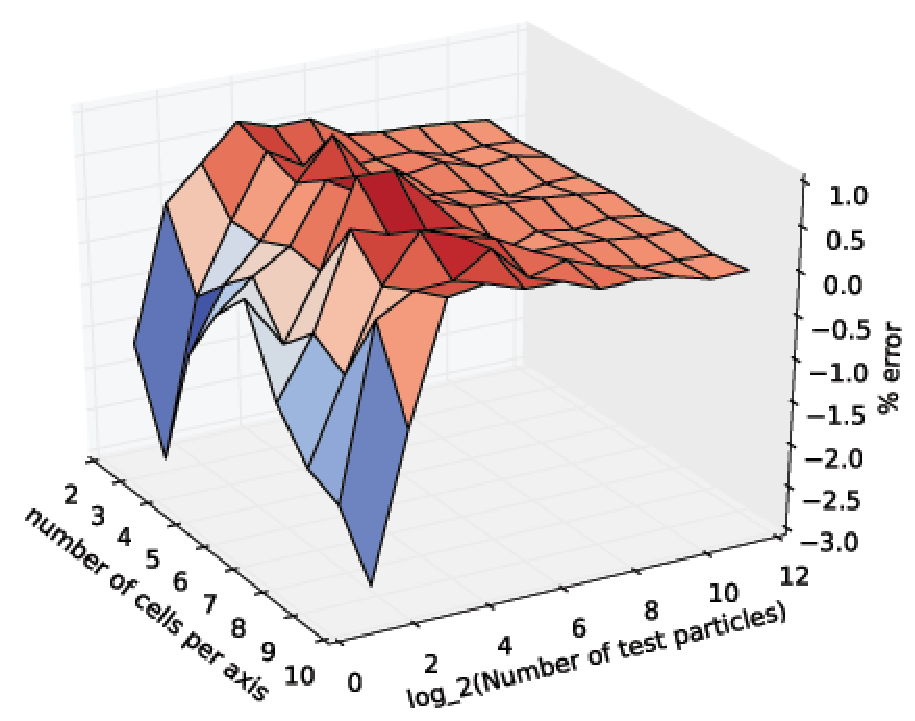
\includegraphics[width=0.525\textwidth]{gfx/HomoError}}%
\subfloat[IP err]{\label{fig:b}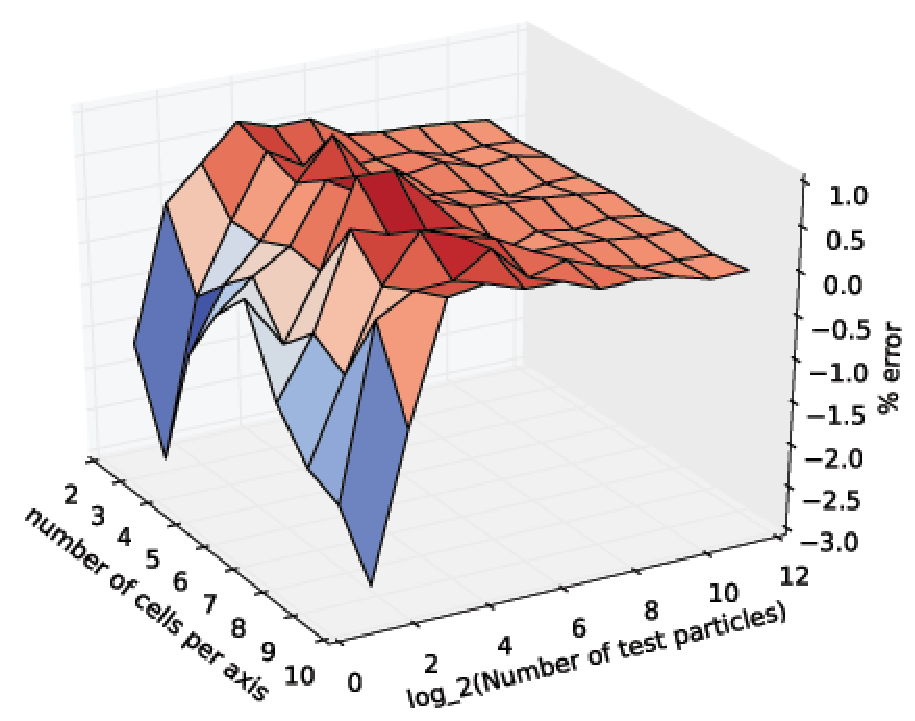
\includegraphics[width=0.525\textwidth]{gfx/HomoError}}%
\subfloat[Quad err]{\label{fig:c}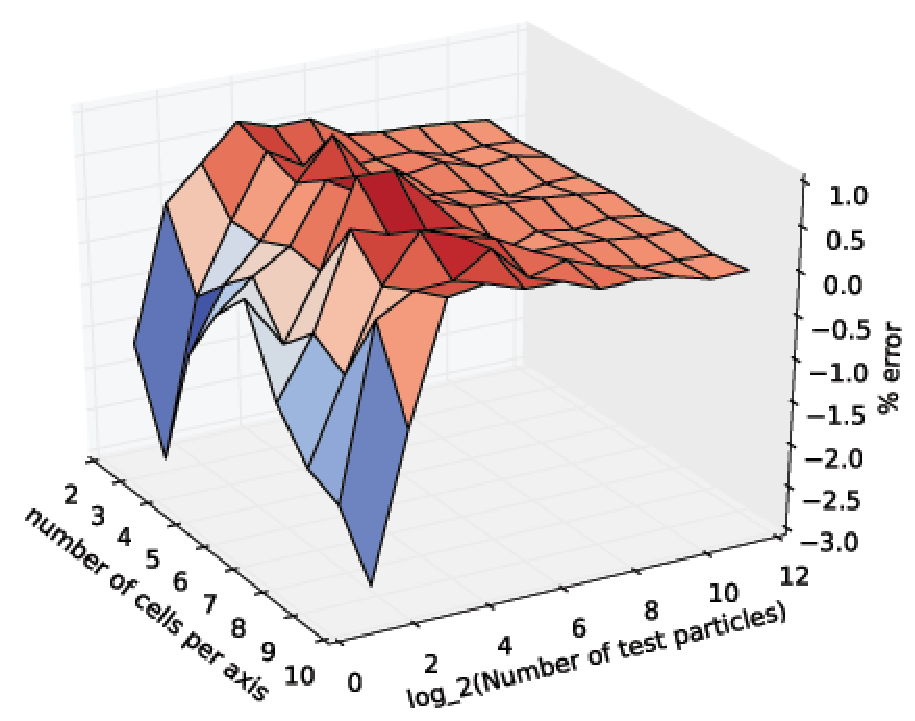
\includegraphics[width=0.525\textwidth]{gfx/HomoError}}%
}
\caption{Error of DSMC method as a function of test particle number and cell number.}\label{fig:dsmccolerr}
\end{figure}

Figure \ref{fig:dsmchomoerr} shows how well the DSMC method performs over a wide range of test particle and cell numbers in a homogeneous gas. 
We can see in the corner the method beginning to fail. 
This is the region where, on average, we have less than two test particles per cell. 
This means that there is not enough atoms to perform a collision within a cell. 
One way to avoid this (which has not been implemented here) is to search neighbouring cells for collision pairs when a partner can not be found in the current cell.
The main thing to observe here is the increase in the error as the number of test particles is reduced.

Smaller cells -> larger fluctuations.

Not adaptive since slowly changing cloud.


%----------------------------------------------------------------------------------------

\section{Thermalisation} 

Now that we are convinced an atomic gas, simulated with the DSMC method, has a physically correct collision rate, we must confirm that collisions distribute energy as we expect.
\marginpar{Thermalisation is the generic name for all kinds of processes giving rise to relaxation towards thermal equilibrium starting from a non-equilibrium situation \cite{Walraven2010}.} 
The perfect way to test this is through an investigation of \emph{thermal relaxation} or the process of thermalisation through elastic collisions.
There are many ways that a system can be out of thermal equilibrium, but here I will consider two scenarios that have generally accepted solutions to which we can compare our simulations.

\subsection{Thermal Relaxation after a Thermal Perturbation} \label{sec:walravenTherm}

The simplest example for rethermalisation\footnote{A more common terminology for thermal relaxation is rethermalisaiton \ie\,to return to the thermal distribution.} is somewhat reminiscent of evaporative cooling, that is the case of simply perturbing equilibrium by adding a small number of atoms whose average energy is different to that of the bulk gas\footnote{Obviously evaporative cooling is simply the removal of atoms whose total energy is different from the average of the bulk.}.
In \cite{Walraven2010} Walraven shows that the rethermalisation time\footnote{That is the $1/e$ time.}, $\tau_\mathrm{th}$, is given by
\begin{equation}
    \tau_\mathrm{th} = 2\left(\gamma + 3/2\right)\tau_{c}. \label{eq:walravenRetherm}
\end{equation}
Using the values for the trapping parameter, $\gamma$, given in \autoref{tab:collisionrates} we find the rethermalisation time in a homogeneous, IP and quadrupole trap to be 3, 6 and 9 times the collision time in each trap respectively.

Anderlini and Gu\'ery-Odelin \cite{Anderlini2006} have taken this analysis one step further, considering the effect of including all partial waves in the collision integrals has on a homogeneous box trap and a harmonic potential.
Interestingly in the limit of constant cross section the results for the homogeneous trap reduces to that given in \autoref{eq:walravenRetherm} with $\gamma=0$, ($\tau_\mathrm{th}=3\tau_\mathrm{c}$).
In fact they go on to show that for the harmonic trap the rethermalisation time is longer by a factor of 2, which again, agrees with \autoref{eq:walravenRetherm} for $\gamma=3/2$, ($\tau_\mathrm{th}=6\tau_\mathrm{c}$).

Before we tackle this scenario numerically the reader might be a little confused by the above result. 
Looking at equation \autoref{eq:walravenRetherm} it is quite clear that as the trapping parameter, $\gamma$, increases the number of collision required for rethermalisation increases.
Aderlini et al. explain this best when they say
\begin{displayquote}
    \dots the fact that the space of configuration is larger for a nonhomogeneous gas, and that the thermalization affects both the space and velocity degrees of freedom.
\end{displayquote}
We can understand this statement better if we consider an effective volume in configuration space, $V_\mathrm{cs}$, (analogous to the effective volume in real space, $V_{e}$)
\begin{equation}
    V_\mathrm{cs} = \int \exp\left[ -\frac{H( \mathbf{r}, \mathbf{v})}{k_B T}\right]\,d\mathbf{r}d\mathbf{v} = V_e \left(\frac{3\pi m}{k_B T}\right)^{3/2}.
\end{equation}
So we can see that for a given temperature the region occupied in configuration space increases with the effective volume, which \autoref{tab:collisionrates} shows increases with $\gamma$.
Again this might make the reader uncomfortable, we seem to have convincingly shown that tighter trapping potentials take longer to rethermalise. 
We stated in \autoref{sec:collisionRates} that evaporative cooling, a process driven by thermal relaxation is more efficient in tighter trapping potentials \ie\,larger trapping parameters.
So how can this be?
As I will show in \autoref{sec:evaporation}, even though these traps take longer to rethermalise they have greater gains in density for a given number of lost atoms during evaporation.

\begin{figure}
\hspace{-8em}
\makebox[1.8\linewidth][l]{%
\centering
\subfloat[Walraven homegeneous gas thermalisation. $\tau_{c}^{-1} / \tau^{-1} = 1.2$ should equal 3?]{\label{fig:walravenHomo}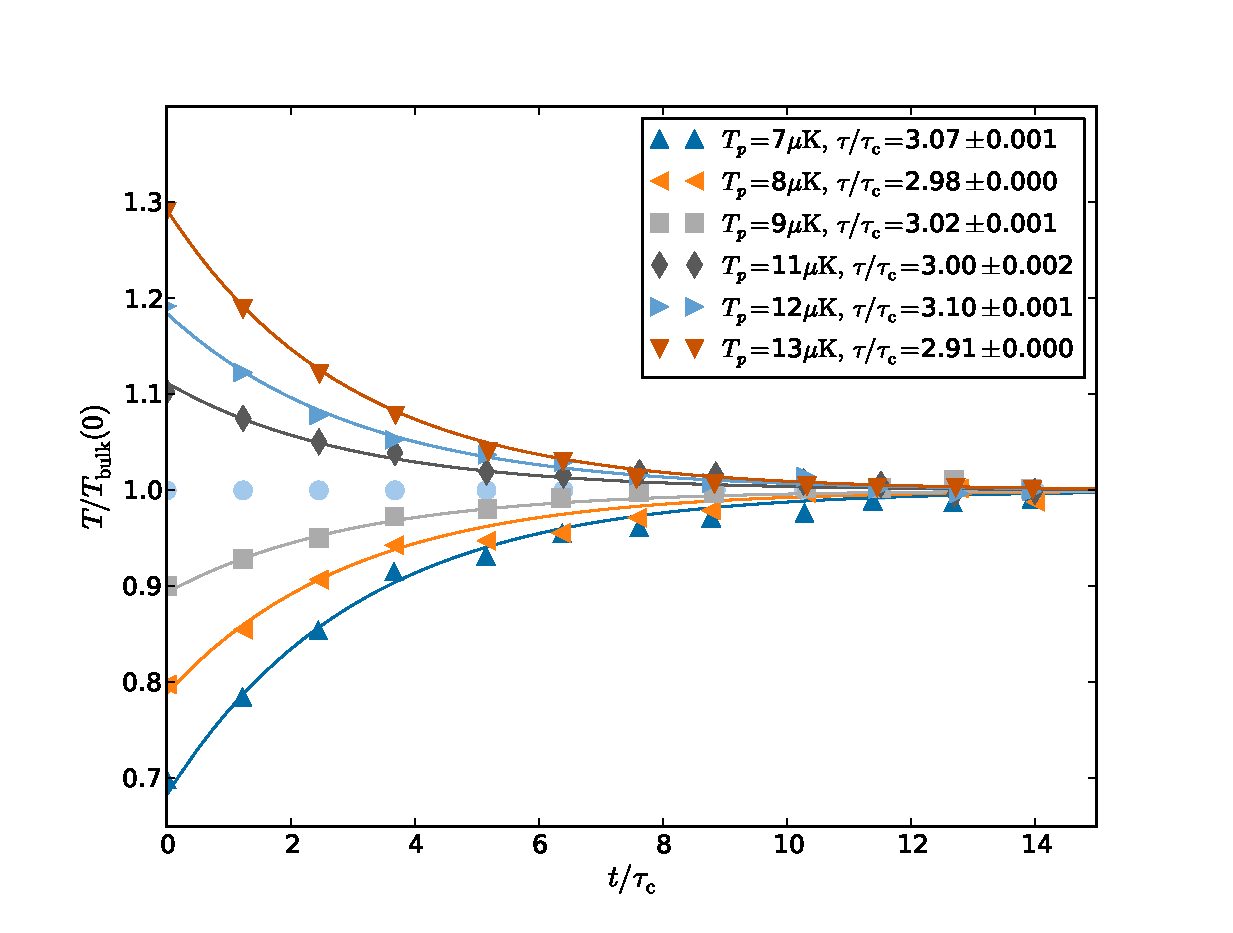
\includegraphics[width=0.525\textwidth]{gfx/Thermalisation/walravenHomo}}\quad
\subfloat[Walraven ip gas thermalisation. $\tau_{c}^{-1} / \tau^{-1} = 1.6$ should equal 6?]{\label{fig:walravenIP}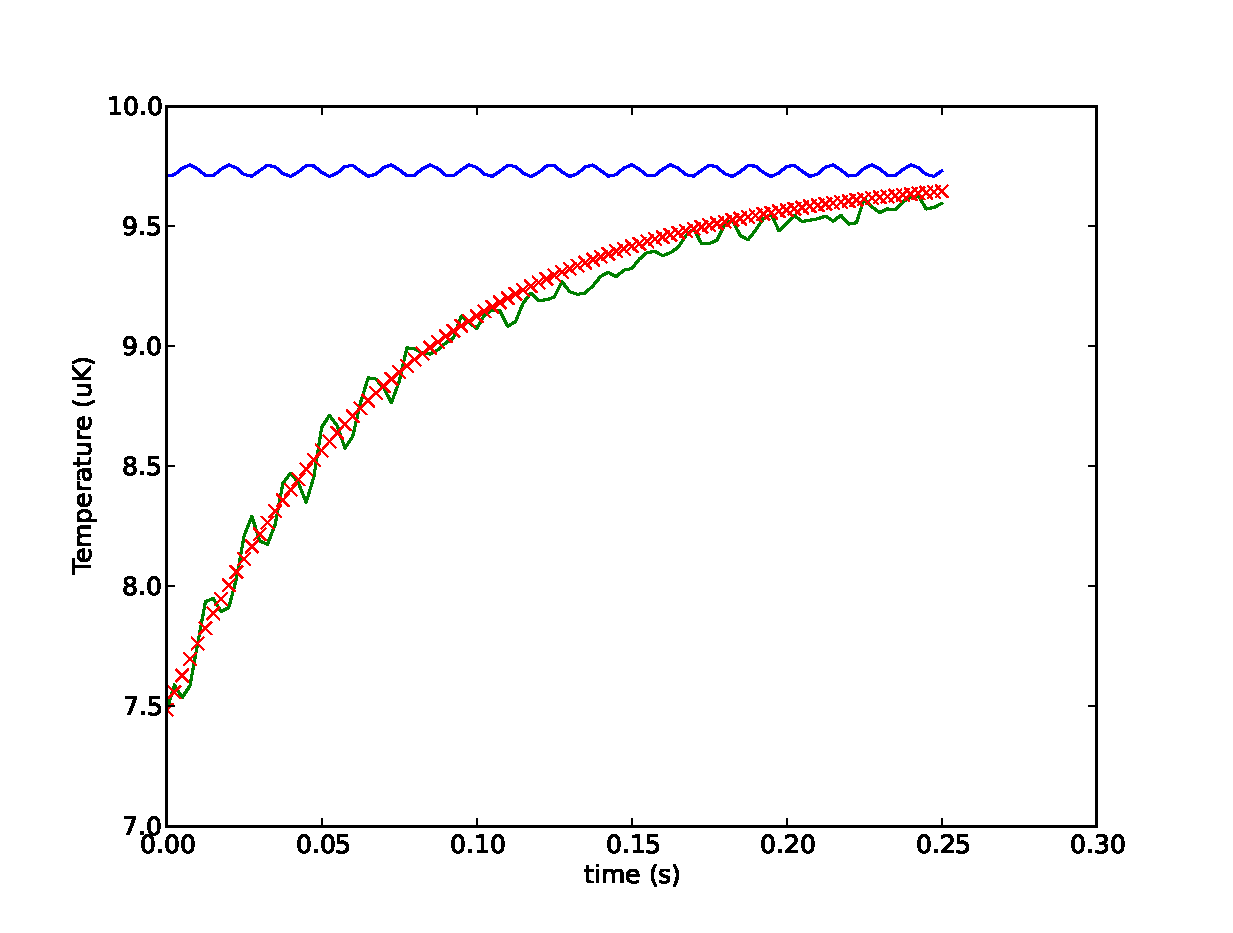
\includegraphics[width=0.525\textwidth]{gfx/Thermalisation/walravenIP}}\quad
\subfloat[Walraven quad gas thermalisation. $\tau_{c}^{-1} / \tau^{-1} = 10.45$ should equal 9?]{\label{fig:walravenQ}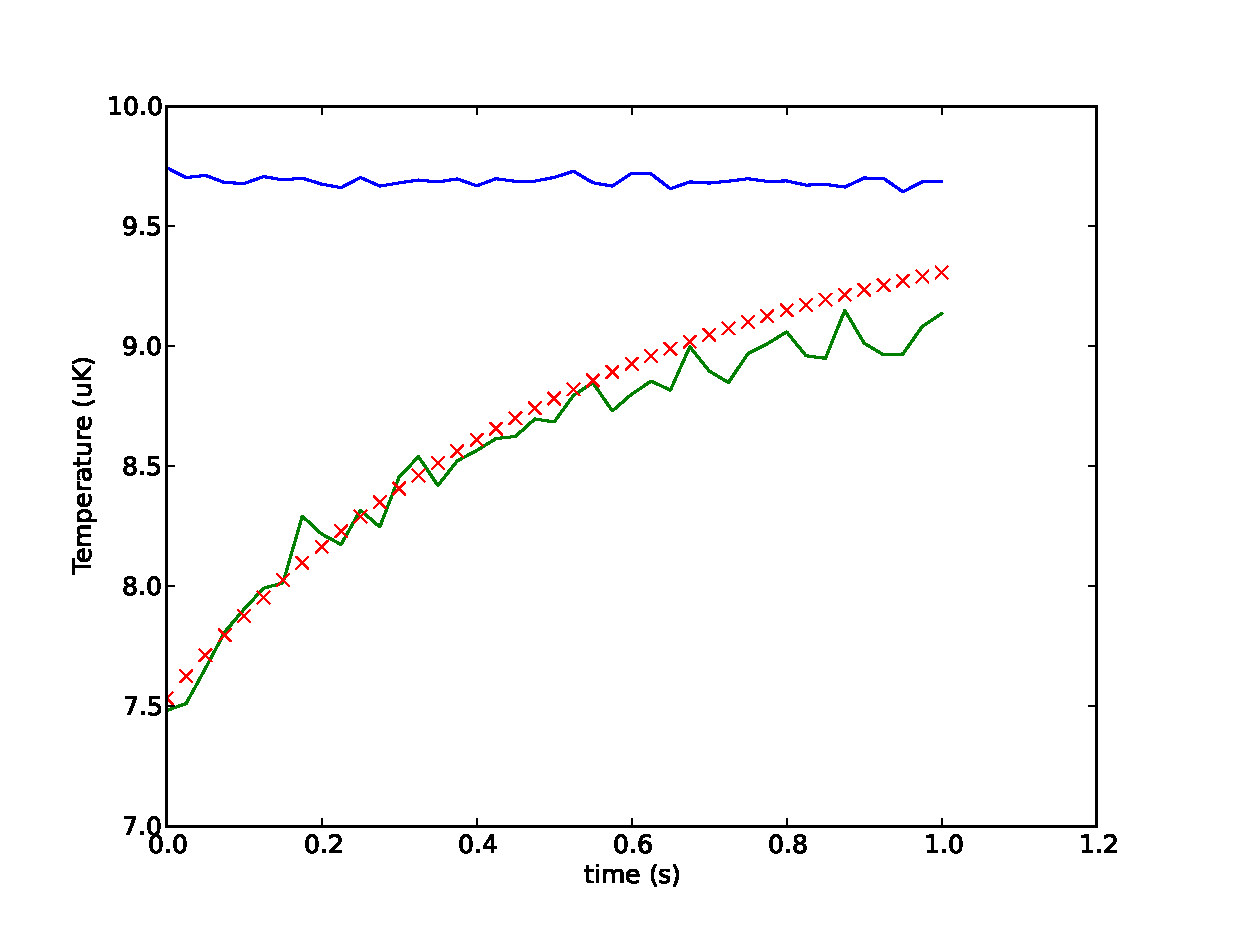
\includegraphics[width=0.525\textwidth]{gfx/Thermalisation/walravenQuad}}%
}
\caption{Walraven rethermalisation. I want to do this simulation for some different perturbation temperatures. One more higher and one lower too.}\label{fig:walravenTherm}
\end{figure}

In \autoref{fig:walravenTherm} we have simulated a million physical atoms, $N_P=10^6$, at $10\,\mu \mathrm{K}$ in three different trapping potentials: homogeneous, IP and quadrupole. 
Each gas began in an initially thermal distribution with 1\% of the particles at set to have an average temperature of $7,8,9,11,12,13\,\mu\mathrm{K}$.
\marginpar{When choosing the initial perturbed distribution we must keep in mind the virial theorem \cite{}. The key result here is that in a thermal distribution we have $\langle E_p \rangle = \frac{2\gamma}{3} \langle E_k \rangle = \gamma k_B T$. So when choosing the width for the spatial distribution we must keep in mind the effective power of the trapping potential. }
For each simulation we have chosen the trapping parameters such that the collision rate was approximately 25 collisions per atom per second, as this number is similar to atoms of this temperature in an evaporation experiment.
We used one million test particle, $N_T=10^6$, in each simulation so that the ratio of physical atoms to test particles was one, $\alpha=1$.

For the homogeneous gas simulation shown in \autoref{fig:walravenHomo} I set the width of the box containing the atoms to be $100\,\mu \mathrm{m}$ in each direction. 
This corresponds to a collision rate of $24.64\,\mathrm{s}^{-1}$.
I found the thermalisation occurred in $3.14\pm 0.02$ collision times, closely resembling the result in \autoref{eq:walravenRetherm}.

For the Ioffe Pritchard trap simulation shown in \autoref{fig:walravenIP} we set $B_0=0.01\,\mathrm{T}$, $B'=33.54\,\mathrm{Tm}^{-1}$ and $B''=75,000\,\mathrm{Tm}^{-2}$ which equates to a ${B_{\rho}}''=75,000\,\mathrm{Tm}^{-2}$. 
Choosing these trapping parameters gives a collision rate of $24.72\,\mathrm{s}$.
I found the thermalisation occurred in $6\pm 0.1$ collision times, again, in perfect agreement with \autoref{eq:walravenRetherm}.

Finally in the quadrupole trap simulation shown in \autoref{fig:walravenQ} we set $B_z'=2.8\,\mathrm{Tm}^{-1}$ resulting in a collision rate of $25.48\,\mathrm{s}$.
I found the thermalisation occurred in $9\pm 0.1$ collision times, again, in perfect agreement with \autoref{eq:walravenRetherm}.

We can note from all simulations shown in \autoref{fig:walravenTherm} that the thermalisation time appears to be independent of the size of the perturbation. 
Not truue large perturbations tend to thermalise i different times.

Also talk about cell number, correct resolution and not thermalising in the correct time.

\subsection{Monroe Thermalisation}

Another interesting experiment that has been investigated in some depth is the rethermalisation of a directional anisotropy. 
In these experiments the kinetic energy is changed in one cartesian direction only (the spatial distribution is reshaped accordingly), creating a directional anisotropy in the distribution.
This squeezed distribution is then allowed to rethermalise through elastic collisions.
The original theoretical development of Myatt \cite{Myatt1997} predicts that in a harmonic trap the thermalisation time for a directional anisotropy is approximately 2.7.
This result has been used to experimentally determine the collision cross section, $\sigma$, of atoms in ultra-cold gas experiments \cite{Monroe1993, Davis1995}. 

Snoke and Wolfe \cite{Snoke1989} also considered the rethermalisation of homogeneous gas with a non-thermal initial distribution.
They found that no matter what the initial distribution their simulated gases always tended to a Maxwell-Boltzmann distribution in less than 5 collisions.

Wu and Foot \cite{Wu1996} have repeated these simulations (both those of Myatt and Snoke and Wolfe) using the DSMC method.
Their simulations agreed with the predictions of Myatt for the case of the harmonic trap, while they found that directional anisotropies in a homogeneous gas thermalised in fewer collisions than in a trapped gas (as we might expect given the result in \autoref{eq:walravenRetherm}).

Here I have extended this investigation to consider the rethermalisation times in our three favourite trapping potentials: homogeneous, Ioffe Pritchard and quadrupole.
As we saw in \autoref{sec:walravenTherm} we can't expect the thermalisation time to be the same in different trapping potentials.
In fact, when the perturbation was kept constant, the thermalisation time was purely a function of the trapping parameter, $\gamma$.

\begin{figure}
\hspace{-12em}
\makebox[1.8\linewidth][l]{%
\centering
\subfloat[Monroe homegeneous gas thermalisation. $\tau_{c}^{-1} / \tau^{-1} = 0.77$]{\label{fig:monroeHomo}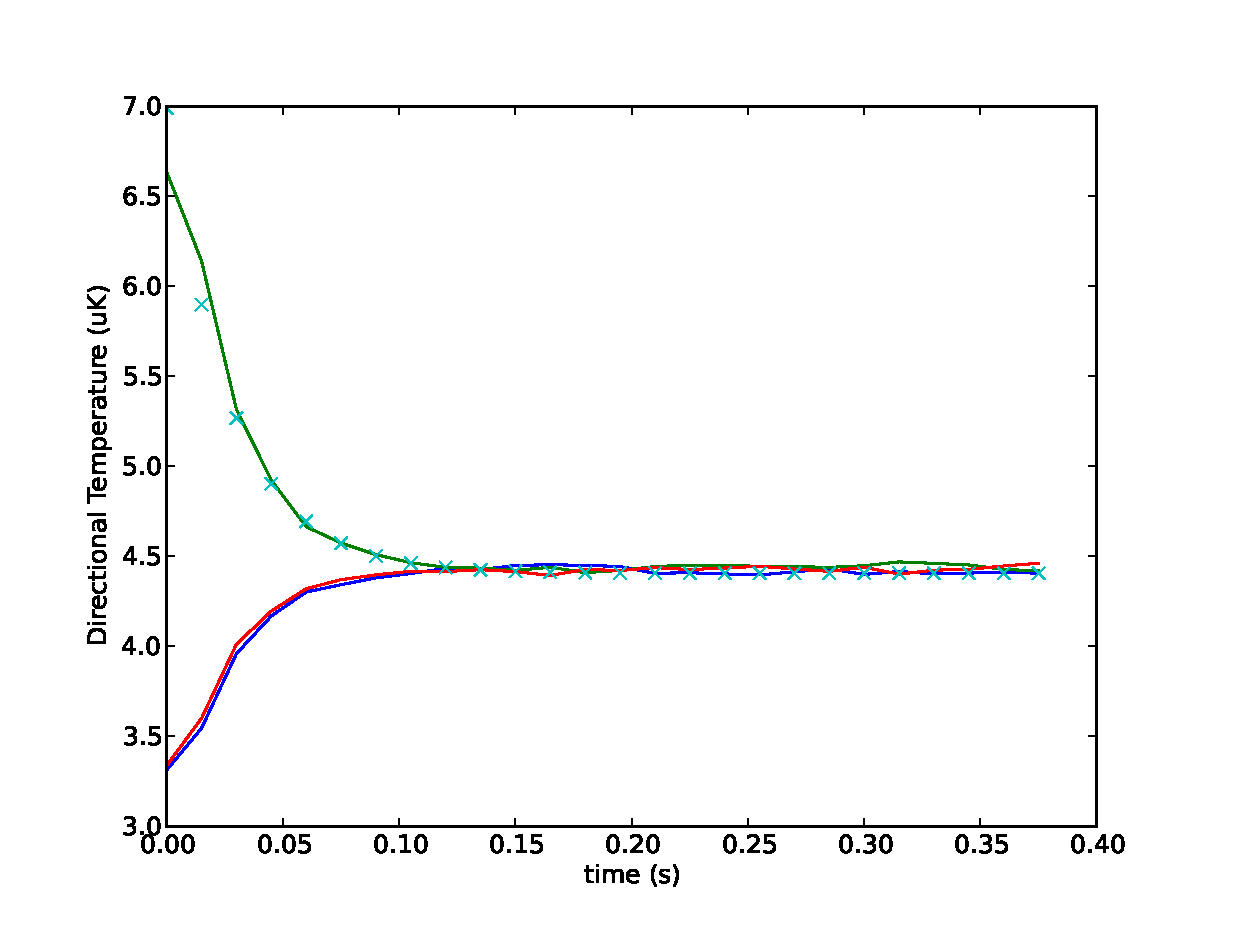
\includegraphics[width=0.525\textwidth]{gfx/Thermalisation/monroeHomo}}\quad
\subfloat[Walraven homegeneous gas thermalisation. $\tau_{c}^{-1} / \tau^{-1} = 2.21$]{\label{fig:monroeIP}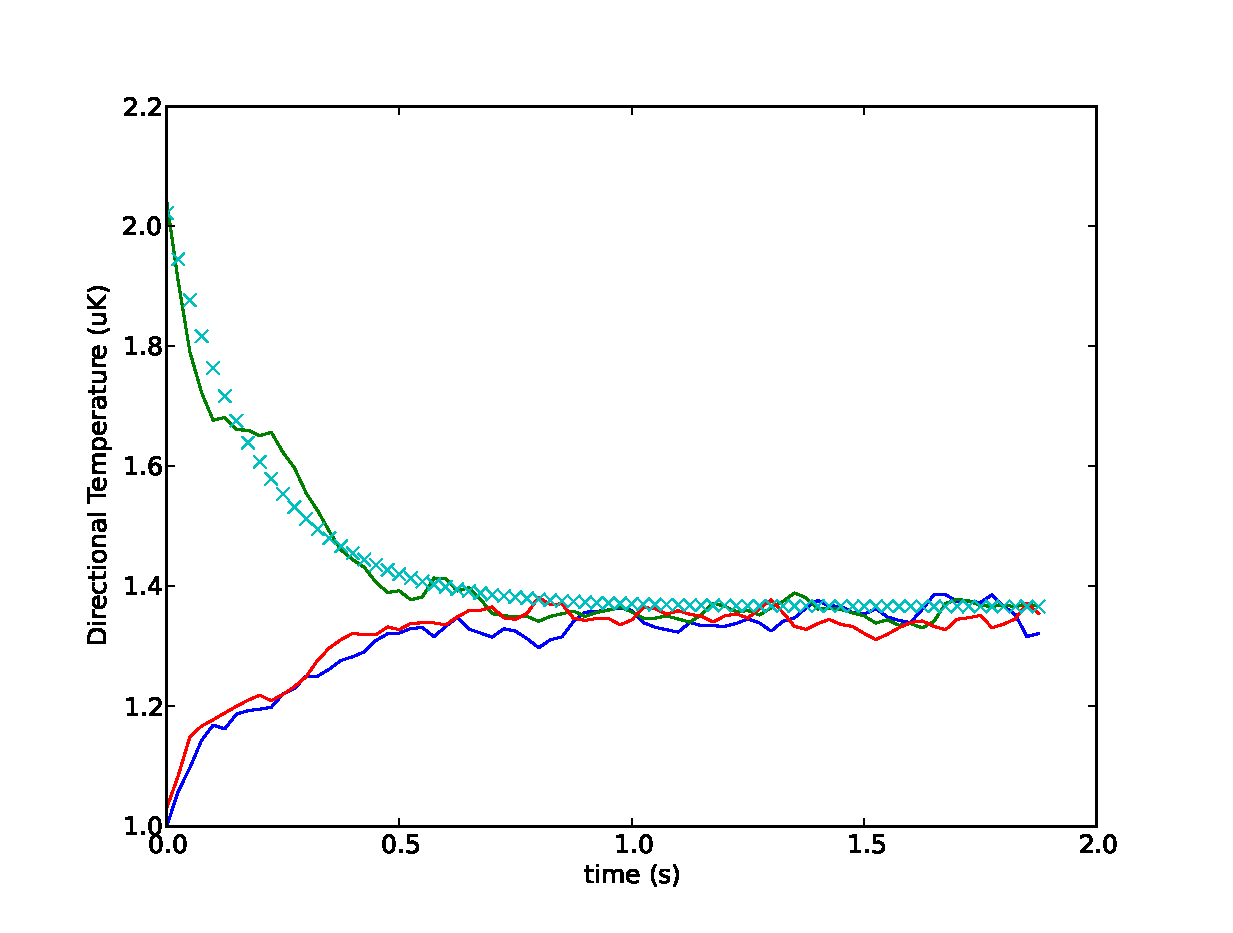
\includegraphics[width=0.525\textwidth]{gfx/Thermalisation/monroeIP}}\quad
\subfloat[Walraven quad gas thermalisation. $\tau_{c}^{-1} / \tau^{-1} = 6.09$]{\label{fig:monroeQ}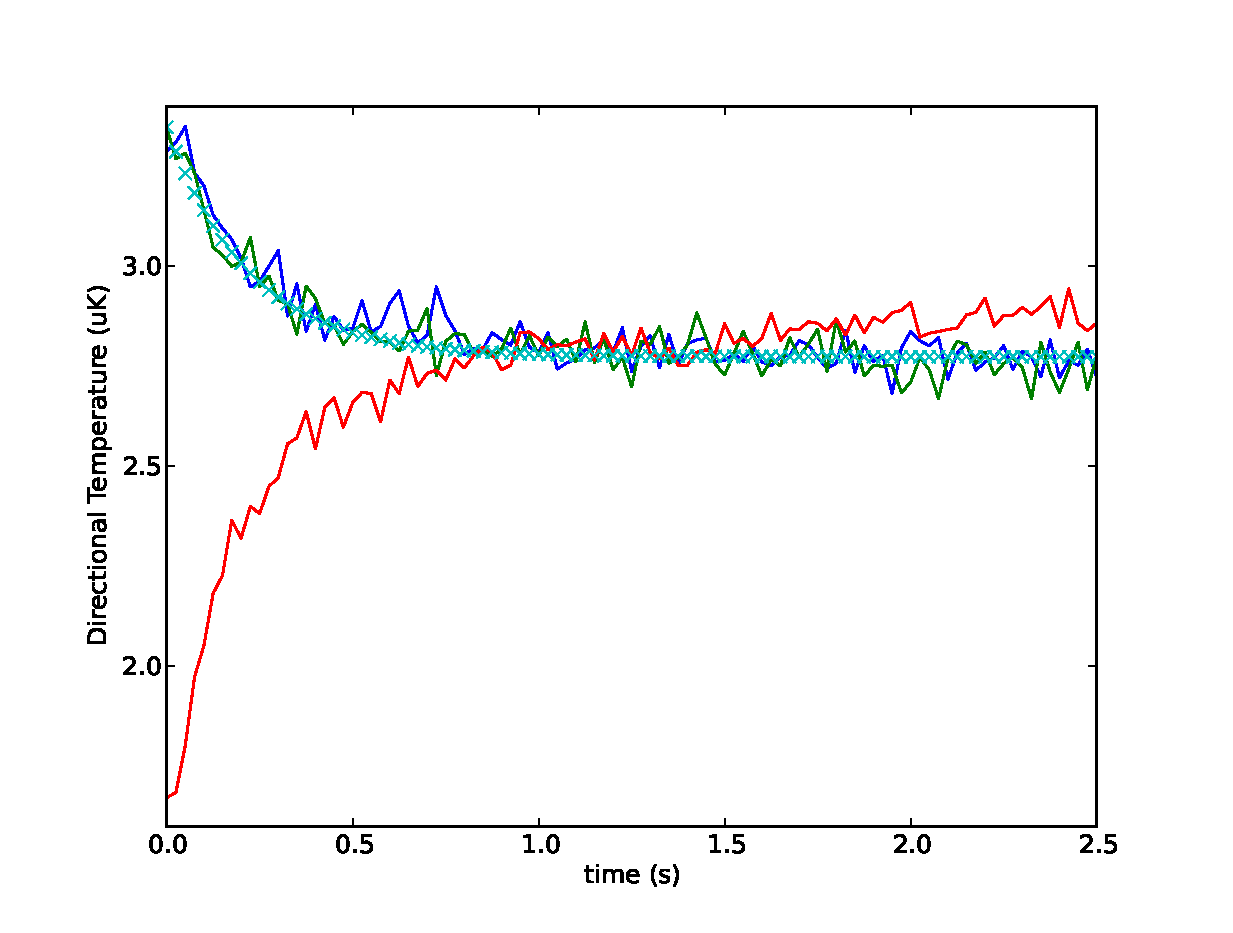
\includegraphics[width=0.525\textwidth]{gfx/Thermalisation/monroeQuad}}%
}
\caption{Walraven rethermalisation. I want to do this simulation for some different perturbation temperatures. One more higher and one lower too.}\label{fig:monroeTherm}
\end{figure}

Also do it for different temperatures or trap numbers.

*** MUST REDO ALL OF THESE SIMULATIONS WITH COLLISIONS WORKING CORRECTLY (I.E. WITH THE NEW SORTING FIX IMPLEMENTED). ***
\marginpar{Comment on directional temperatures being a useful tool for checking that collisions are working effectively. }
%----------------------------------------------------------------------------------------

\section{Evaporation} \label{sec:evaporation}

Compare some results to those predicted by the theory of walraven \cite{Walraven2010} and the other guy \cite{Luiten1996} . 

Say something about the ability to accurately simulate evaporation being important for ensuring the simulation of energy distribution during majorana loss.

As demonstrated by Wu et al \cite{Wu1996, Wu1997} we can use the DSMC method to simulate evaporative cooling.
There has been a lot of theoretical investigation into the evolution of cold gases under forced evaporative cooling \cite{Davis1995, Luiten1996, Holland1996}, giving us a good basis for analysis.
We will use the results of Luiten et al \cite{Luiten1996} to validate to our simulations.
In their work Luiten et al find that the rate of change of total energy due to evaporation is given by 
\begin{equation}    
    \dot{E} = \left( \eta + \frac{W_{\mathrm{ev}}}{V_{\mathrm{ev}}}\right) \dot{N} k_B T, \label{eq:evapEnergy}
\end{equation}
where the effective volume for elastic collisions leading to evaporation, $V_\mathrm{ev}$, is given by
\begin{equation*}
    V_\mathrm{ev} = \frac{\Lambda}{k_B T} \int_0^{\epsilon_t} \rho(\epsilon)\left[\left(\epsilon_t-\epsilon-k_B T\right)e^{-\epsilon/k_B T} + k_B T e^{-\eta}\right]\,d\epsilon
\end{equation*}
and the volume $W_\mathrm{ev} = V_\mathrm{ev} - X_\mathrm{ev} $, with
\begin{equation*}
    X_\mathrm{ev} = \frac{\Lambda}{k_B T} \int_0^{\epsilon_t} \rho(\epsilon)\left[k_B Te^{-\epsilon/k_B T}  - \left(\epsilon_t-\epsilon+k_B T\right)e^{-\eta}\right]\,d\epsilon.
\end{equation*}
If we use the expression for an isotropic power law potential, \autoref{eq:powerlaw} from \autoref{sec:collisionRates}, we can find a (rather complicated) expression for this ratio of volumes
\begin{equation*}
    \frac{X_\mathrm{ev}}{V_\mathrm{ev}} = \frac{2 \left(2 (2 \gamma +2 \eta +5) \eta ^{\gamma +\frac{3}{2}}+e^{\eta } \left((2 \gamma +3) (2 \gamma +5) \Gamma \left(\gamma +\frac{3}{2},\eta \right)-4 \Gamma \left(\gamma +\frac{7}{2}\right)\right)\right)}{e^{\eta } (-2 \gamma +2 \eta -5) \left((2 \gamma +3) (2 \gamma +5) \Gamma \left(\gamma +\frac{3}{2},\eta \right)-4 \Gamma \left(\gamma +\frac{7}{2}\right)\right)-2 (2 \gamma +5)^2 \eta ^{\gamma +\frac{3}{2}}},
\end{equation*}
where $\Gamma\left[a,z\right] = \int_z^\infty t^{a-1}e^{-t}\,dt$ is the incomplete gamma function and $\Gamma\left[a\right] = \int_0^\infty t^{a-1}e^{-t}\,dt$ is the Euler gamma function.
It might not be immediately obvious from the equation above, but for a given $\gamma$ this ratio has a maximum of 1 at $\eta=0$ and is a monotonically decreasing function of $\eta$.
I have included this to illustrate a rather unintuitive result.
That is that the rate of change of the total energy for an evaporatively cooled gas is not only a function of the evaporation parameter $\eta$, but also a function of the trapping parameter $\gamma$.
Perhaps if we reflect on the thermalisation experiments we have done in the previous \autoref{sec:walravenTherm} and \autoref{sec:monroeTherm} it is not so surprising that this is the case.

If we now differentiate the equation for the total energy of the gas, $E=\left(\frac{3}{2} + \gamma\right)Nk_BT$, with respect to time and combine it with \autoref{eq:evapEnergy} we can show
\begin{equation}
    \frac{\dot{T}}{T} = \left(\frac{\eta + \frac{W_\mathrm{ev}}{V_\mathrm{ev}}}{\frac{3}{2}+\gamma}-1\right) \frac{\dot{N}}{N}. \label{eq:tempEvap}
\end{equation}
Keeping in mind the maximal value for $W_\mathrm{ev} / V_\mathrm{ev}$ is 1 we can see from the above that we require $\eta > \gamma + 1/2$ for the temperature to decrease as the number of atoms decreases. 
Further more we can note the larger $\eta$ is the more efficient the evaporative cooling will be \ie a smaller loss of atoms will result in a larger decrease in temperature.

We can also investigate how the density of the gas changes with the number of atoms.
Recall in section \autoref{sec:collisionRates} we claimed the density would \emph{increase} as we \emph{removed} atoms (how can this be?!).
Using the relationship $N=n_0V_e$ and the subsequent derivative $\dot{N} = \dot{n}_0V_e + n_0\dot{V}_e$, and combining this with the results from \autoref{tab:collisionrates} and \autoref{eq:tempEvap} we have
\begin{equation}
    \frac{\dot{n}_0}{n_0} = \left(1-\gamma\left(\frac{\eta + \frac{W_\mathrm{ev}}{V_\mathrm{ev}}}{\frac{3}{2}+\gamma}-1\right)\right) \frac{\dot{N}}{N}. \label{eq:densEvap}
\end{equation}
Thus we see that for the density of the gas to increase as the number of atoms decreases we require that $\eta > \gamma + 3/2 + 3/2\gamma$. 
It is clear from \autoref{eq:densEvap} that the larger $\gamma$ is the greater increase in density we will have for a given loss of atoms.

Finally we can see how the degeneracy parameter, $D=n_0\Lambda^3$, changes with the loss of atoms
\begin{equation}
    \frac{\dot{D}}{D} = \left(\gamma -\eta -\frac{W_\mathrm{ev}}{V_\mathrm{ev}} +\frac{5}{2}\right) \frac{\dot{N}}{N}.
\end{equation}
So for $\eta > \gamma + 3/2$ we will have an increase in the degeneracy parameter as the number of atoms decreases.
Here is the definitive result that drives the desire to evaporate in a quadrupole potential.
We can see that the larger $\gamma$ is the greater the increase in the degeneracy parameter will be for a given $\eta$.
Thus if we can use a quadrupole trap, with $\gamma = 3$, we will reach the quantum limit with the minimum atom loss.

%----------------------------------------------------------------------------------------

\section{DSMC simulations of Evaporation} \label{sec:dsmcevaporation}

Armed with the relationships from \autoref{sec:evaporation} we can investigate the accuracy of the DSMC when applied to the evaporative cooling of cold atoms.

\begin{figure}[bth]
\myfloatalign
\subfloat[$\eta$ should equal 7, here it is equal to 7.86 ]
{\label{fig:dsmchomoerr}
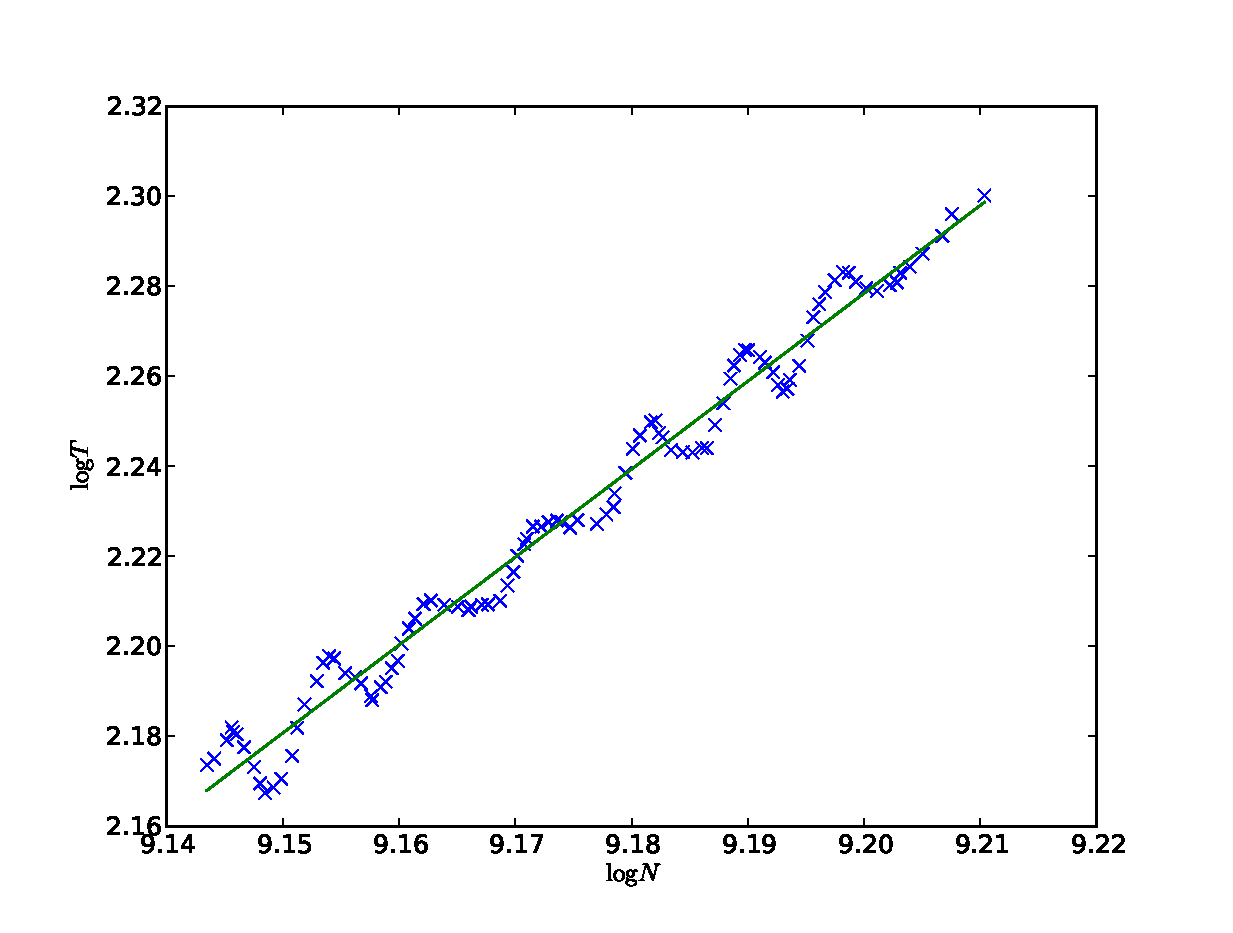
\includegraphics[width=.45\linewidth]{gfx/Evaporation/evapIP}} \quad
\subfloat[I want this to be a plot of n0 vs N.]
{\label{fig:dsmcquaderr}
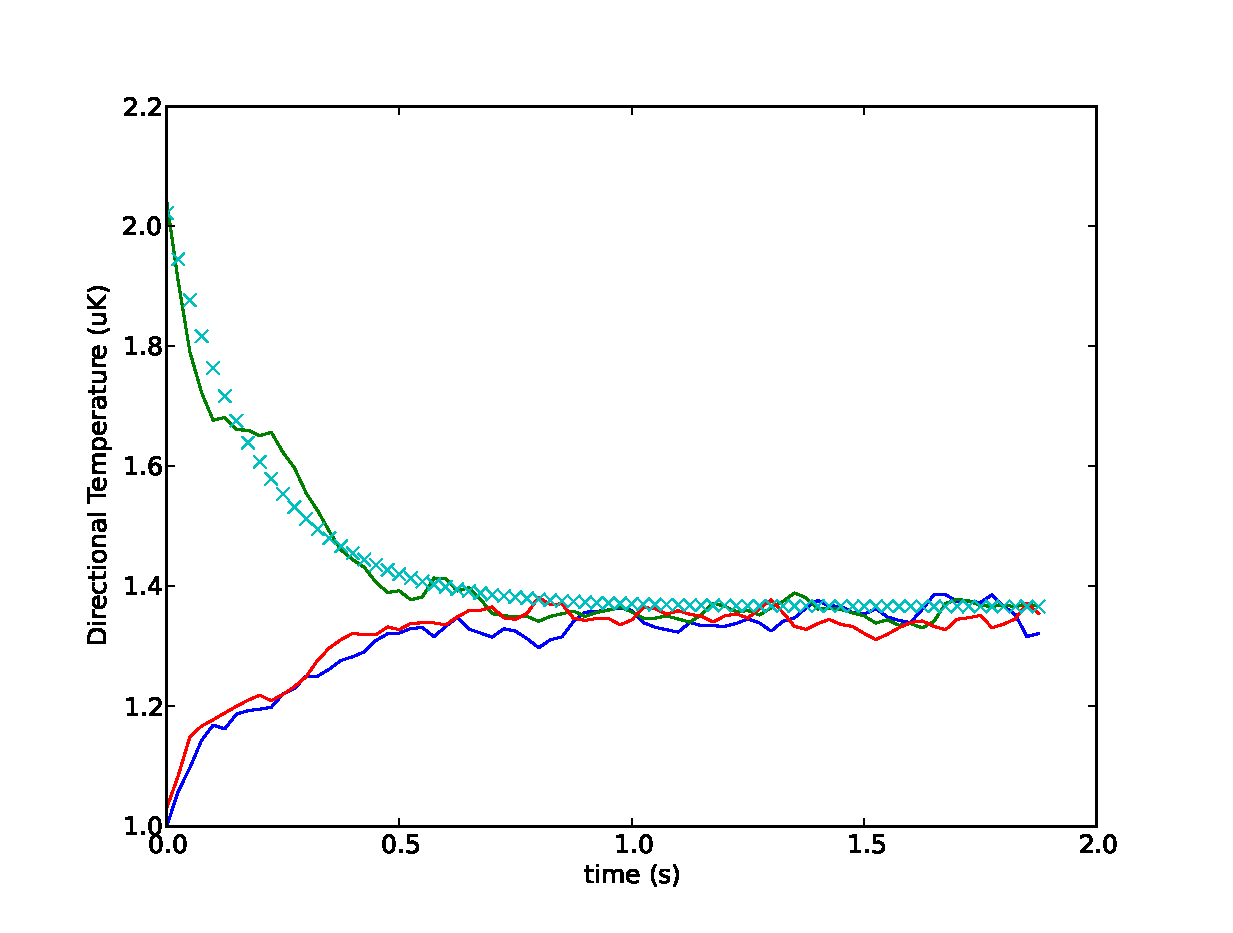
\includegraphics[width=.45\linewidth]{gfx/Thermalisation/monroeIP}}
\subfloat[Not sure what plot tp put here]
{\label{fig:dsmcquaderr}
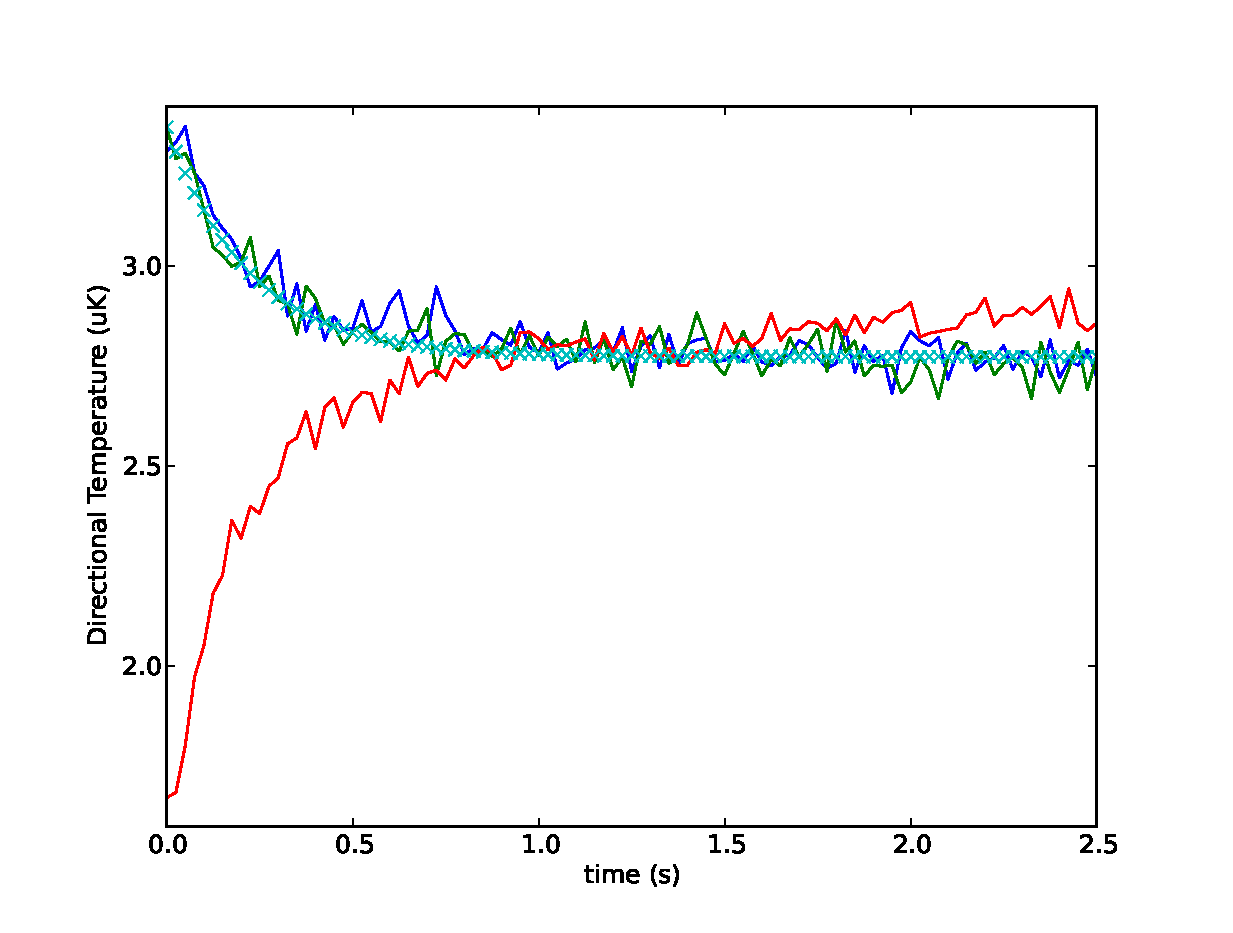
\includegraphics[width=.45\linewidth]{gfx/Thermalisation/monroeQuad}}
\caption[]{IP trap evaporation.}\label{fig:dsmccolerr}
\end{figure}

\begin{figure}[bth]
\myfloatalign
\subfloat[$\eta$ should equal ?(check the paper), here it is equal to 5 ]
{\label{fig:dsmchomoerr}
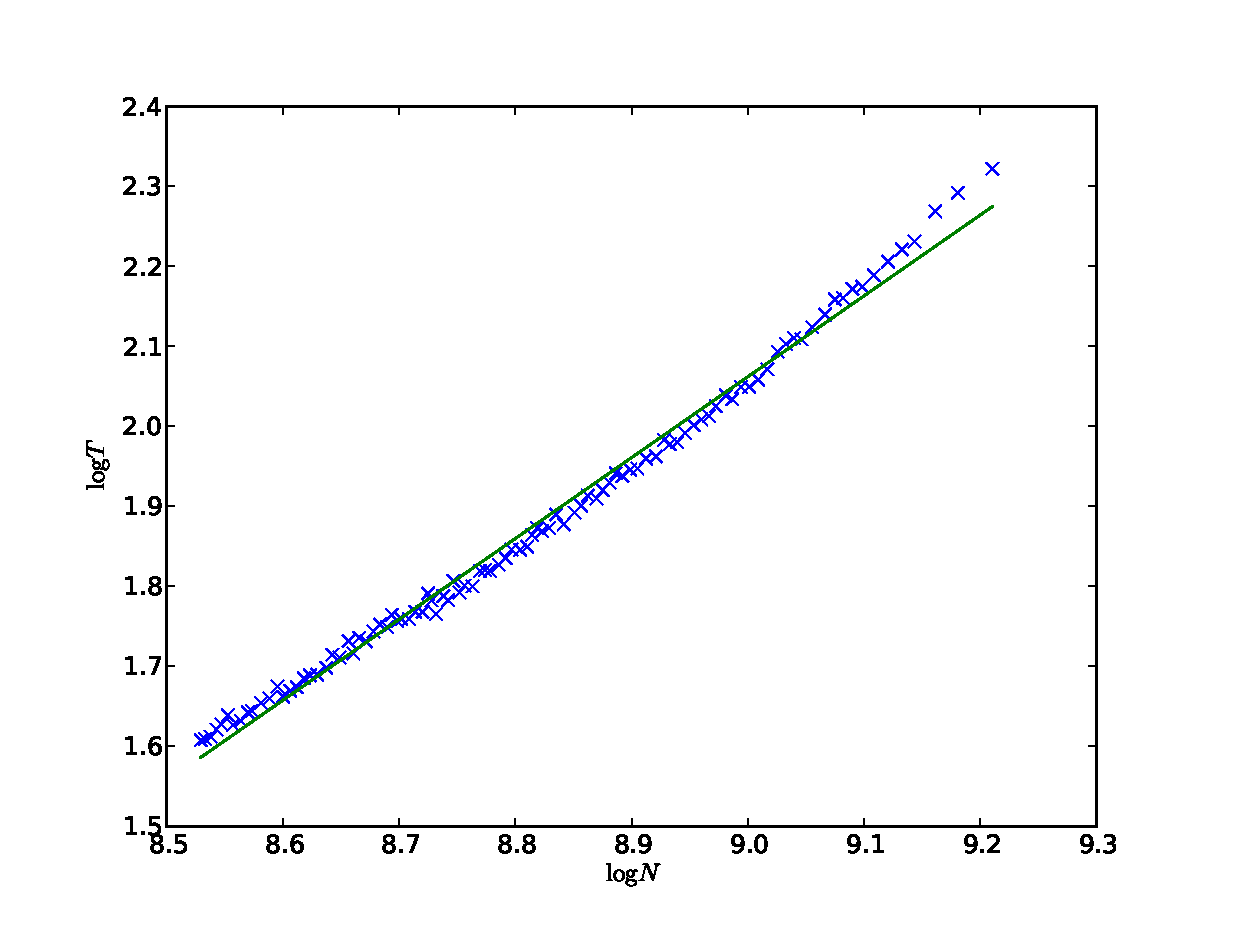
\includegraphics[width=.45\linewidth]{gfx/Evaporation/evapQuad}} \quad
\subfloat[I want this to be a plot of n0 vs N.]
{\label{fig:dsmcquaderr}
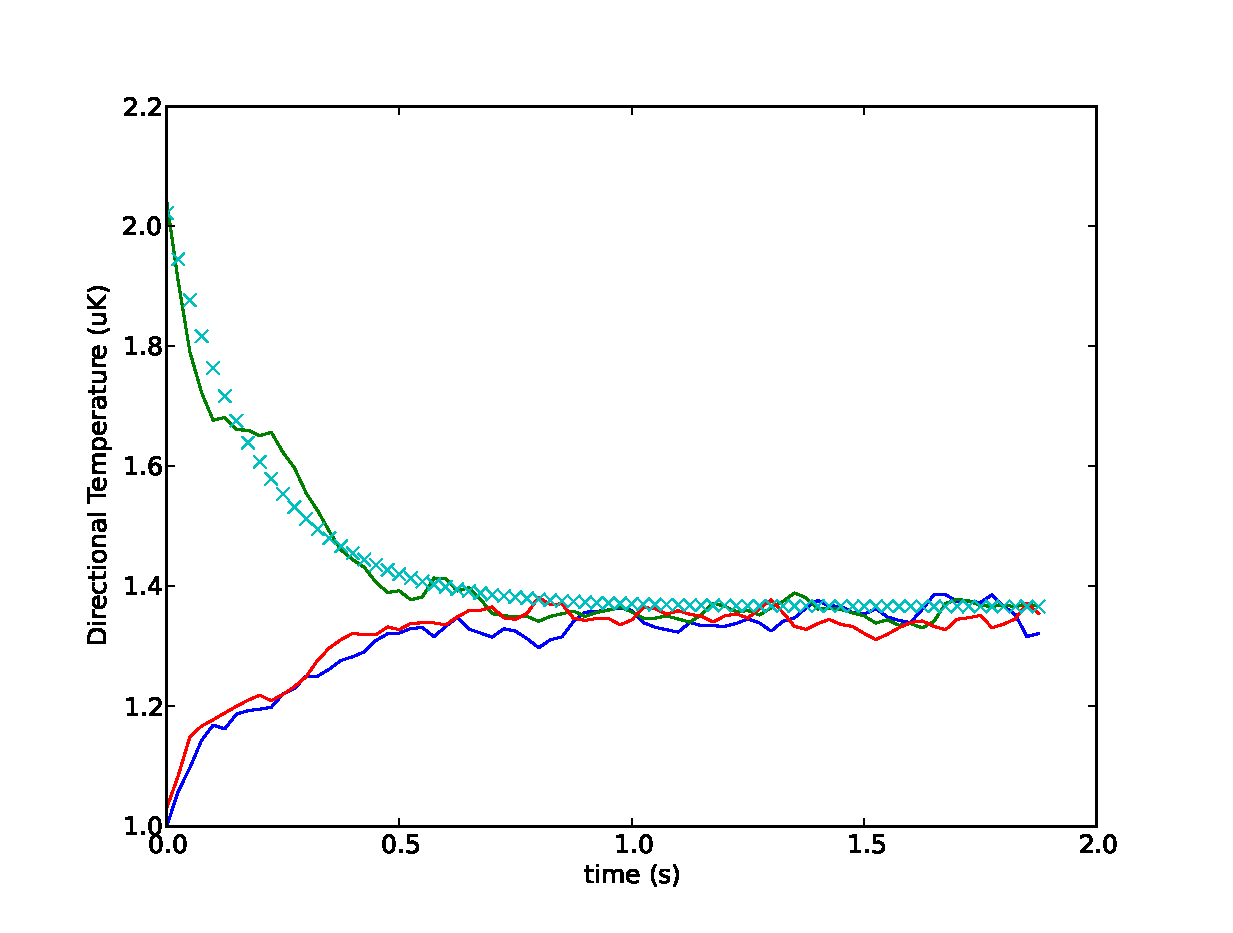
\includegraphics[width=.45\linewidth]{gfx/Thermalisation/monroeIP}}
\subfloat[Not sure what plot tp put here]
{\label{fig:dsmcquaderr}
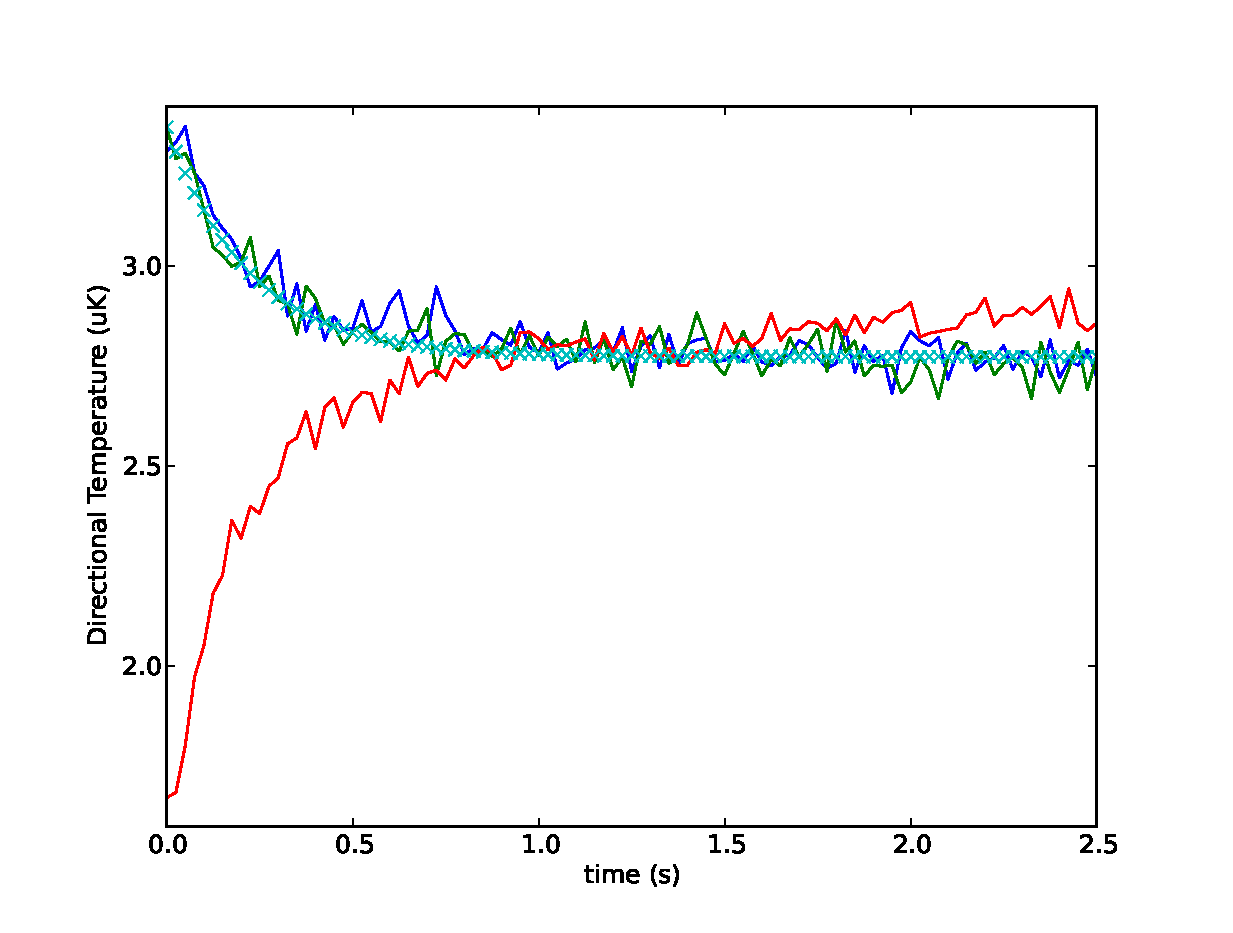
\includegraphics[width=.45\linewidth]{gfx/Thermalisation/monroeQuad}}
\caption[]{Quadrupole trap evaporation.}\label{fig:dsmccolerr}
\end{figure}

\section{Adiabaticity}

Have a look at squeezing the magnetic trap both diabaticaly and adiabatically. % INHOMOGENEOUS GAS
% Chapter X

\chapter{Majorana Interulde} % Chapter title

\label{ch:majinter} % For referencing the chapter elsewhere, use \autoref{ch:dsmcehr} 

%-----------------------------------------------------------------------------------------

General scope for the problem.

Inadequacies in alternative approaches.

Majorana's approach does not require the extension into the imaginary time domain nor does he make dodgey mistakes in an attempt to engineer the solution.

%-----------------------------------------------------------------------------------------

\section{Derivation of the Differential Equation}

To illustrate the theory of an avoided crossing we will consider the case of a static 2-level atom in a dynamic field. 
The interaction Hamiltonian for a magnetic dipole in a magnetic field is $\widehat{H}_{B} = -\hat{\boldsymbol{\mu}} \cdot \boldsymbol{B}$, written in matrix form is
\begin{equation}
	\widehat{H}_{B} = \hbar \gamma \begin{bmatrix} B_{z} & B_{x} - i B_{y}\\
											B_{x} + i B_{y} & -B_{z} \end{bmatrix}, \label{Eq:MagHam}
\end{equation}
where $\gamma = g_{F}\mu_{B}M_{F} / \hbar$ is the gyromagnetic ratio and represents the proportionality between the spin and magnetic moment, $\hat{\boldsymbol{\mu}}$, operators. 
If we choose the ``spin up,'' $\vert\uparrow\rangle$ and ``spin down,'' $\vert \downarrow\rangle$ states as our basis then, the diagonal elements are the energies of our basis (or diabatic) states and the off diagonal elements represent the coupling between states. 
The eigenvalues for the hamiltonian in \eqref{Eq:MagHam} are 
\begin{equation}
	E_{\pm} = \pm \hbar \gamma \sqrt{{B_{x}}^{2} + {B_{y}}^{2} + {B_{z}}^{2}},
\end{equation}
and correspond to the states perfectly aligned (and anti-aligned) with the local magnetic field. 
We can see the effect of the coupling between states in these eigen-energies through the appearance of the term, $\left\vert\Delta\right\vert^{2} = {B_{x}}^{2} + {B_{y}}^{2}$. 
More specifically consider the two situations shown in figure \ref{Fig:AvoidedCrossing}. 
When there is no coupling we get the grey curves and when there is coupling we get the coloured curves \textcolor{red}{(explain)}. 
If we consider a time-dependant magnetic field in which the coupling is constant and the diagonal field changes from large and negative to large positive very slowly (or \emph{adiabatically}) then the system should follow the one of the curves. 
If it goes quickly then it might jump across the gap \textcolor{red}{(this is rubbish)}.

The time-dependant magnetic field discussed in Majorana's paper \cite{Majorana1932} is ${\mathbf B} = \left(A, 0 , -Ct\right)$ and so the corresponding coupled time-dependant Schr\"odinger equations for a spin half particle with $\vert\psi(t)\rangle = c_{1}(t) \vert \downarrow\rangle + c_{2}(t) \vert \uparrow \rangle$, are
\begin{subequations}
\begin{align}
	\dot{c_{1}} &= - \gamma i \left(-Ctc_{1} + Ac_{2}\right),\\
	\dot{c_{2}} &= - \gamma i \left(A c_{1} + Ct c_{2}\right).
\end{align}
\end{subequations}
Using the dimensionless time
\begin{equation}
	\tau = \sqrt{\frac{\gamma \, C}{2}} \, t,
\end{equation}
and the numerical quantity
\begin{equation}
	k = \frac{2\gamma A^{2}}{C},
\end{equation}
which describes the ratio of the atom precession frequency to the rotation frequency of the field direction, we can obtain the coupled differential equations
\begin{subequations} \label{eq:Majprob}
\begin{align}
	\frac{dc_{1}}{d\tau} &= - i \left(-2\tau c_{1} + \sqrt{k}c_{2}\right),\\
	\frac{dc_{2}}{d\tau} &= -i \left(\sqrt{k} c_{1} + 2\tau c_{2}\right).
\end{align}
\end{subequations}
These equations can be further simplified through the application of the integration factor method \cite{Kreyszig2006}, by setting
\begin{equation}
	c_{1} = e^{i\tau^{2}}f, \quad \quad
	c_{2} = e^{-i\tau^{2}}g,
\end{equation}
from which it follows
\begin{subequations}
\begin{align}
	\frac{df}{d\tau} &= -i \sqrt{k} e^{-2i\tau^{2}}g,\\
	\frac{dg}{d\tau} &= -i \sqrt{k} e^{2i\tau^{2}}f. \label{Eq:dgdt}
\end{align}
\end{subequations}
Eliminating $g$, we obtain\footnote{The factor of $4i\tau$ was erroneously printed as $hi\tau$.}
\begin{equation}
	\frac{d^{2}f}{d\tau^{2}} + 4 i \tau \frac{df}{d\tau} + kf = 0. \label{Eq:fDiff}
\end{equation}

%-----------------------------------------------------------------------------------------

\section{Transforming into an Integral Equation}

When obtaining an asymptotic solution to a differential equation it is often preferable to investigate the asymptotic behaviour of an integral solution. 
It is not always possible to obtain an integral solution, but when possible it provides a global solution from which all asymptotic limits can be obtained, and hence connect solutions from one domain to another. 
It is with this motivation that we seek to find an integral representation of equation \eqref{Eq:fDiff}. 
To this end we will assume the solution can be written as an integral of the product between a given kernel $K(s,\tau)$ and some unknown function\cite{White2005} $\chi(s)$
\begin{equation}
	f(\tau) = \int_{C} K(s,\tau) \chi(s) \, ds,
\end{equation}
where $C$ is an arbitrary contour in the complex plane and $K$ and $\chi$ are \emph{complex functions} of the \emph{complex variable} $s$. 
We will use the Fourier Laplace kernel, $K(s,\tau) = e^{s\tau}$ so that the differential equation \eqref{Eq:fDiff} becomes
\begin{equation}
	\int_{C}\chi(s) \left(s^{2}+k\right)e^{s\tau}\, ds + 4i\int_{C}\chi(s)s\tau e^{s\tau} \, ds = 0.
\end{equation}
If we now integrate the second term by parts we have
\begin{equation}
	\left.\int_{C}\left[\left(s^{2}+k-4i\right)\chi(s) - 4is \chi'(s)\right] e^{s\tau}\, ds + s\chi(s)e^{s\tau}\right\vert_{C} = 0.
\end{equation}
Choosing the contour, $C$, such that the boundary term disappears we are left with the differential equation
\begin{equation}
	\left(s^{2}+k-4i\right)\chi(s) - 4is \chi'(s) = 0,
\end{equation}
which is separable and has solution the solution
\begin{equation}
	\chi(s) = As^{(k/4i) - 1}e^{s^{2}/8i},
\end{equation}
so long as $\log_{e}s$ assumes its principle value. 
Here $A$ is a constant of normalisation, to be determined in section \ref{Sec:Asymp}. 
Thus we have 
\begin{equation}
	f(\tau) = A\int_{C}s^{(k/4i)-1}e^{(s^{2}/8i)+s\tau}\, ds, \label{Eq:AsymInt}
\end{equation}
with the boundary condition
\begin{equation}
	\left.s^{k/4i}e^{(s^{2}/8i)+s\tau}\right\vert_{C}=0.
\end{equation}
\textcolor{red}{(for example consider the rays where $\text{Arg} \,s = -\frac{\pi}{4}, \, \frac{3\pi}{4}$.)}

%-----------------------------------------------------------------------------------------

\section{Asymptotic Solution of the Integral} \label{Sec:Asymp}

The simplest technique for obtaining the asymptotic behaviour as $\tau \to +\infty$ of integrals in which the large parameter $\tau$ appears in an exponential
\begin{equation}
	I(\tau) = \int_{a}^{b} h(s) e^{\tau\phi(s)} \, ds,
\end{equation}
is Laplace's method \cite{Bender1999} where we assume $h(s)$ and $\phi(s)$ are \emph{real} and \emph{continuous}. 
The crux of Laplace's method is the idea that if the real continuous function $\phi(s)$ has its \emph{maximum} on the interval $a \le s \le b$ at $t = c$ and if $h(c) \ne 0$, then it is only the \emph{immediate neighbourhood} of $t=c$ that contributes to the full asymptotic expansion of $I(\tau)$ for large $\tau$. 
That is we may approximate the integral $I(\tau)$ by $I(\tau; \epsilon)$ where
\begin{align}
	I(\tau;\epsilon) &= \int_{c-\epsilon}^{c+\epsilon}h(s) e^{\tau\phi(s)}\, ds,\\
	&\approx \int_{c-\epsilon}^{c+\epsilon}\left[h(c) + \left(s-c\right)h'(c) + {\cal O}(s^{2})\right]e^{\tau\left[\phi(c)+\left(s-c\right)\phi'(c) + \frac{1}{2}\left(s-c\right)^{2}\phi''(c)+{\cal O}(s^{3})\right]}\, ds,\\
	&\approx h(c)e^{\tau\phi(c)}\int_{-\infty}^{\infty} e^{\tau\left(s-c\right)^{2}\phi''(s)/2}\, ds, \quad \text{as }\tau \to + \infty. \label{Eq:Laplace}
\end{align}
However we notice straight away that our function $h(s) = s^{(k/4i)-1}e^{s^{2}/8i}$ is not real, nor is the variable of integration, $s$, thus Laplace's method is not directly applicable, we will instead, employ a technique known as the method of steepest descents \cite{Bender1999}. 
The method of steepest descents is a technique for finding the asymptotic behaviour of integrals of the form
\begin{equation}
	I(\tau) = \int_{C}h(s) e^{\tau \rho(s)} \, ds, \label{Eq:SteepestDescent}
\end{equation}
as $\tau \to +\infty$, where $C$ is an integration contour in the complex $s$ plane and $h(s)$ and $\rho(s)$ are \emph{analytic functions} of $s$. 
Here the idea is to use the analyticity of the integrand to justify deforming the contour $C$ to a new contour $C'$ on which $\rho(s)$ has a constant imaginary part. 
Once this has been done, $I(s)$ may be evaluated asymptotically as $\tau \to +\infty$ using Laplace's method. 
To see why, observe that on the contour $C'$ we may write $\rho(s) = \phi(s) + i \psi$, where $\psi$ is a real constant and $\phi(s)$ is a real function. 
Thus, $I(s)$ in \eqref{Eq:SteepestDescent} takes the form
\begin{equation}
	I(s) = e^{is\psi} \int_{C'}h(s) e^{\tau\phi(s)}\, ds.
\end{equation}
In our case we cannot simply use $\rho(s) = s$ since it's maximum is infinite and we expect the integral to be convergent, we instead have to consider the entire exponent $\rho(s) = s^{2}/8i+s\tau$. 
If we plan on using Laplace's method to approximate the integral along the deformed contour then we require that the new contour passes through the stationary point of $\rho(s)$. 
The stationary point of $\rho(s)$ will be at $ s_{\text{st.pt.}} = -4i\tau$. Now we let $s = p + iq$ so that  
\begin{equation}
	\rho(s) = \rho(p,q) = \left[\frac{1}{4}pq + \tau p\right] + i \left[ \frac{1}{8}q^{2} - \frac{1}{8}p^{2} + \tau q\right],
\end{equation}
thus the imaginary part of the exponent at the stationary point is $\Im(\rho(s_{\text{st.pt}})) = \Im(\rho(0,-4\tau)) = -2\tau^{2}$. 
The contours along which the imaginary part of $\rho(s)$ is constant and equal to $\text{Im}(\rho(s_{\text{st.pt.}}))$ are thus given by
\begin{align}
	-2\tau^{2} &= \frac{1}{8}q^{2} + q\tau - \frac{1}{8}p^{2},\\
	\Rightarrow q &= -4\tau \pm p.
\end{align}
These two contours are shown in figure \ref{Fig:ContourPlots}. 
Since we require that the stationary point $s_{\text{st.pt.}}=-4i\tau$ be a maximum we will choose the contour $y=-4\tau-p$ so that we now have
\begin{equation}
	s = -4i \tau + \left(1 - i\right)p, \quad ds = \left(1 - i\right) dp.
\end{equation}
Making this substitution the integral \eqref{Eq:AsymInt} becomes
\begin{equation}
	f(\tau) =A\left(1-i\right)e^{-2i\tau^{2}}\int_{-\infty}^{\infty}\left(-4i\tau + \left(1-i\right)p\right)^{(k/4i)-1}e^{-p^{2}/4}\, dp.
\end{equation}
While $\tau < 0$ we can apply equation \eqref{Eq:Laplace} directly to find
\begin{align}
	f(\tau) &\approx A\left(1-i\right)e^{-2i\tau^{2}}\left(-4i \tau\right)^{k/4i-1}\int_{-\infty}^{\infty}e^{-p^{2}/4}\, dp, \quad \text{as } \tau \to -\infty\\
	&= 2A\left(1-i\right)\sqrt{\pi}e^{-2i\tau^{2}}\left(-4i \tau\right)^{k/4i-1}, \quad \text{as } \tau \to -\infty.
\end{align}
In the limit $\tau \to -\infty$ we find $f(\tau) = 0$ and using equation \eqref{Eq:dgdt} we have 
\begin{align}
	g(\tau) &= \int_{-\infty}^{\tau}2kAi\left(1-i\right)\sqrt{\pi}\left(-4i \tau' \right)^{k/4i-1}\, d\tau', \quad \text{as } \tau \to -\infty\\
	&= 2A\left(1+i\right)\sqrt{\pi}\left(-4 \tau' \right)^{k/4i}e^{k\pi/8} , \quad \text{as } \tau \to -\infty.
\end{align}
We can see that if $\left\vert g\right\vert^{2} = 1$ as $\tau \to - \infty$ we require $A = \sqrt{k}e^{-k\pi/8}/(2(1+i)\sqrt{\pi})$.
When $\tau >0$ the integration contour will have to cross a branch cut along the negative real axis caused by the fractional powers of $s$. 
In this case we will follow the path indicated in figure \ref{Fig:IntegrationPaths}. 
So now let
\begin{align}
	f(\tau) &= \int_{\gamma_{1}} + \int_{\gamma_{2}} + \int_{\gamma_{3}} + \int_{\gamma_{4}} + \int_{\gamma_{5}},\\
	&= f_{1} + f_{2} + f_{3} + f_{4} + f_{5} .
\end{align}
Can show $f_{1}$ and $f_{3}$ tend to zero (at least in the limit $\tau \to 0$). Along $\gamma_{2}$ we let $s = pe^{i \pi}$ so that $ds = e^{i \pi}dp$ and
\begin{equation}
	f_{2} = \frac{\sqrt{k} e^{-k\pi/8}}{2\left(1+i\right)\sqrt{\pi}}\int_{-4\tau}^{\epsilon} p^{(k/4i)-1}e^{k\pi/4}e^{(p^{2}/8i) -p\tau}\, dp.
\end{equation}
Similarly along $\gamma_{4}$ we let $s = pe^{-i\pi}$ so that $ds = e^{-i\pi}dp$ and
\begin{equation}
	f_{4} = -\frac{\sqrt{k} e^{-k\pi/8}}{2\left(1+i\right)\sqrt{\pi}}\int_{-4\tau}^{\epsilon} p^{(k/4i)-1}e^{-k\pi/4}e^{(p^{2}/8i) -p\tau}\, dp.
\end{equation}
Now adding $f_{2}$ and $f_{4}$ together we have
\begin{align}
	f_{2} + f_{4} &= \frac{\sqrt{k} e^{-k\pi/8}}{2\left(1+i\right)\sqrt{\pi}}\int_{-4\tau}^{\epsilon} p^{(k/4i)-1}e^{(p^{2}/8i) -p\tau}\left(e^{k\pi/4}-e^{-k\pi/4}\right)\, dp,\\
	&= \frac{\sqrt{k} e^{-k\pi/8}}{\left(1+i\right)\sqrt{\pi}}\sinh\left(\frac{k\pi}{4}\right)\int_{-4\tau}^{\epsilon} p^{(k/4i)-1}e^{(p^{2}/8i) -p\tau}\, dp,\\
	&= \frac{\sqrt{k} e^{-k\pi/8}}{\left(1+i\right)\sqrt{\pi}}\sinh\left(\frac{k\pi}{4}\right)\int_{-4\tau}^{\epsilon} p^{(k/4i)-1}e^{-p\tau}\left(1 + \frac{p^{2}}{8i} + {\cal O}(p^{4})\right)\, dp.
\end{align}
Looking at the above equation it is clear that if we make the substitution $p\tau = p'$ so that $dp = \tau^{-1}dp'$ we have will have (to the highest order in $\tau$) the integral form of the gamma function so that
\begin{equation}
	f_{2}+f_{4} = \frac{\sqrt{k} e^{-k\pi/8}}{\left(1+i\right)\sqrt{\pi}}\sinh\left(\frac{k\pi}{4}\right)\tau^{-k/4i}\Gamma\left(\frac{k}{4i}\right).
\end{equation}
We will also have the contribution from the saddle point and will be the same as for the $\tau < 0$ case so 
\begin{equation}
	f_{5} = -i\sqrt{k}e^{k\pi/8-2i\tau^{2}}\left(-4i \tau\right)^{-1-k/4i}, \quad \text{as } \tau \to \infty.
\end{equation}
The $\gamma_{1}$ contour will follow the same derivation as the $\gamma_{5}$ except that it's maximum is at $x=-4\tau$ so the Taylor series expansion must be made about this maximum. 
Thus we have
\begin{equation}
	f_{1} = -i\sqrt{k}e^{k\pi/8-2i\tau^{2}}\left(-4 \tau\right)^{-1-k/4i}, \quad \text{as } \tau \to \infty,
\end{equation}
which will decay exponentially as $\tau \to \infty$, faster than $f_{5}$.
Adding all of our results together we find\footnote{The $\tau^{-k/4i}$ was erroneously printed as $e^{-k/4i}$.} in the limit as $\tau \to \infty$
\begin{equation}
	f(\tau) =  \frac{\sqrt{k} e^{-k\pi/8}}{\left(1+i\right)\sqrt{\pi}}\sinh\left(\frac{k\pi}{4}\right)\tau^{-k/4i}\Gamma\left(\frac{k}{4i}\right),
\end{equation}
and 
\begin{equation}
	g(\tau) = (4\tau)^{k/4i}e^{-k\pi/4}.
\end{equation}

%-----------------------------------------------------------------------------------------

\section{Conclusion}

The probability of the spin adiabatically flipping will be given by $\left\vert g \right\vert^{2} = e^{-k\pi/2}$ as $\tau \to \infty$. \textcolor{red}{(Explain the changing sign of the magnetic field swaps the basis vectors.)}

%----------------------------------------------------------------------------------------

\section{Majornan Spin Flips}
\begin{equation}
    \frac{\partial}{\partial t} \label{eq:Majprob}
\end{equation}

Talk about Majorana problem, history, derive formula etc

%----------------------------------------------------------------------------------------

\section{Landau Zener Formula}

Content

\section{Loss Rates 'n' Stuff}

derive the loss rate formulae used in all the literature.  % Majorana Interlude
% Chapter X

\chapter{DSMC WITH SPIN - EHRENFEST} % Chapter title

\label{ch:dsmcehr} % For referencing the chapter elsewhere, use \autoref{ch:dsmcehr} 

To include the effects of Majorana spin flips in our DSMC simulations we will obviously have to develop some semiclassical method \ie simulate the positions of the atoms classically using the DSMC method and simulate the internal state of the atom with a quantum mechanical approach.
One such approach would be to use the Ehrenfest theorem \cite{Ehrenfest1927} to calculate the average force applied to an atom based on its current internal state (I have given a brief pseudo-code in listing \ref{lst:Ehrenfest}).
Using this method we would evolve the internal state of the atom using the Schr\"odinger equation then, using the internal state of the atom, we can calculate the expectation value of the force to use in evolving the position of the atom.

Unfortunately this technique is not a viable solution, as we will demonstrate in this chapter.
While we are able to capture some of the interesting physics (usually short term) of the Majorana spin flip using the Ehrenfest approach, it just fails over long simulation periods.


%----------------------------------------------------------------------------------------

\section{Simulating Schr\"odinger Equation}

To make use of the proposed Ehrenfest method (EM) we need to be able to accurate solve the Sch\"odinger equation.
Some of the more straight forward approached might be to apply a finite difference technique directly to the pde, however these methods are not generally conservative \cite{?}.
In fact the techniques that are considered more stable generally have some non-physical numerical dissipation as a results of the approximations made \cite{?} (or even show?).

The approach we have employed here, and in chapter \ref{ch:dsmcmcwf}, is to make use of the unitary time evolution operator \cite{?}.
The main benefit of this approach is, as the name suggests, the operator is unitary and hence inherently conserves probability.
The unitary time evolution operator is defined as follows
\begin{equation}
    \widehat{U}(t_0,t_0+\Delta t) = \exp\left[-\frac{\imath}{\hbar}\int_{t_0}^{t_0+\Delta t} \widehat{H}(t)\,dt \right]. \label{eq:timeEvolution}
\end{equation}
That is for a time dependant Hamiltonian we can evolve the state of our wavefunction, $\vert \psi \rangle$, through a moment of time $\Delta t$, through the application of the time evolution operator, $\widehat{U}$,
\begin{equation*}
    \ket{ \psi (t_0+\Delta t) } = \widehat{U}(t_0,t_0+\Delta t) \ket{ \psi (t_0) }.
\end{equation*}
This method is especially useful for our two level system as we can explicitly derive an expression for the $2\times2$ matrix form of $\widehat{U}$.
Recall from section \ref{sec:intromag} that the Hamiltonian for a magnetic moment in a magnetic field is given by
\begin{equation*}
    \widehat{H} = -\hat{\boldsymbol{\mu}} \cdot \mathbf{B},
\end{equation*}
which can be expressed in matrix form as
\begin{equation*}
    \widehat{H} = \frac{1}{2}g_s\mu_B \begin{bmatrix} B_z & B_x - \imath B_y \\
                                                      B_x + \imath B_y & -B_z \end{bmatrix}.                                          
\end{equation*}
In general the magnetic field components are functions of position, which, for the atoms is a function of time.
For a general magnetic field we do not know explicitly what the time dependance will be and so we will not be able to explicitly integrate the Hamiltonian as required by equation \eqref{eq:timeEvolution}.
\marginpar{Make a side note about higher order integration.}
So we will have to make the assumption that our time steps are very small, $\Delta t \ll 1$, so that over the time step the Hamiltonian remains relatively constant.
In this limit we have, $\int\widehat{H}\,dt = \widehat{H}\Delta t$, so that the time evolution operator becomes
\begin{align}
    \widehat{U}(t_0,t_0+\Delta t) &= \exp\left[  -\imath\frac{g_s\mu_B\Delta t}{2 \hbar} \begin{bmatrix} B_z & B_x - \imath B_y \\
                                                      B_x + \imath B_y & -B_z \end{bmatrix} \right],\\
                &= \begin{bmatrix} \cos\theta - \imath n_z \sin\theta & -\left(n_y+\imath n_x\right)\sin\theta \\
                                   \left(n_y-\imath n_x\right)\sin\theta & \cos\theta + \imath n_z \sin\theta\end{bmatrix}, 
\end{align}
where $\theta = g_s \mu_B \Delta t \vert \mathbf{B} \vert / 2\hbar$ and $n_k = B_k / \vert \mathbf{B} \vert$ are the directional components of the magnetic field normal vector.
This simple closed form expression makes it very easy to implement the unitary evolution operator method numerically.

%------------------------------------------------

\section{Schr\"odinger Simulations}

To test out this technique lets just numerically solve the original Majorana problem \eqref{eq:Majprob}.
In figure \ref{fig:majprob} I have simulated two scenarios: a spin flip (figs \ref{fig:labframeFlip}, \ref{fig:rotframeFlip}) and a not flip (figs \ref{fig:labframeNoFlip}, \ref{fig:rotframeNoFlip}).
Each scenario is plotted in two seperate refernce frames: the laboratory frame and the co-rotating frame.
The laboratory frame is the frame in which the spin up direction is aligned with the $z$-axis, the co-rotating frame is the frame in which the spin up direction is aligned with the magnetic field.
\marginpar{We find the spin up and spin down components in the co-rotating frame by projecting onto the "local" magnetic field. We do this using the projection operator, $ \ket{\phi_{\uparrow,\downarrow}} = \widehat{P}_{\uparrow,\downarrow} \ket{\Psi}$, where the projection operator is given by $\widehat{P} = ??$.}
The laboratory frame is the frame in which the differential equation is set, however in this frame it can become a little confusing about wether a particular spin state is flipped our not.
In both of the simulations the direction of the magnetic field changes at $t=0$, so the orientation of the spin up direction in the lab frame also changes.
In the co-rotating frame it is always clear which state is the spin up state.

\begin{figure}
\hspace{-6em}
\makebox[1.8\linewidth][l]{%
\centering
\subfloat[Lab frame flip, $B_t=1\times10^{-7}$]{\label{fig:labframeFlip}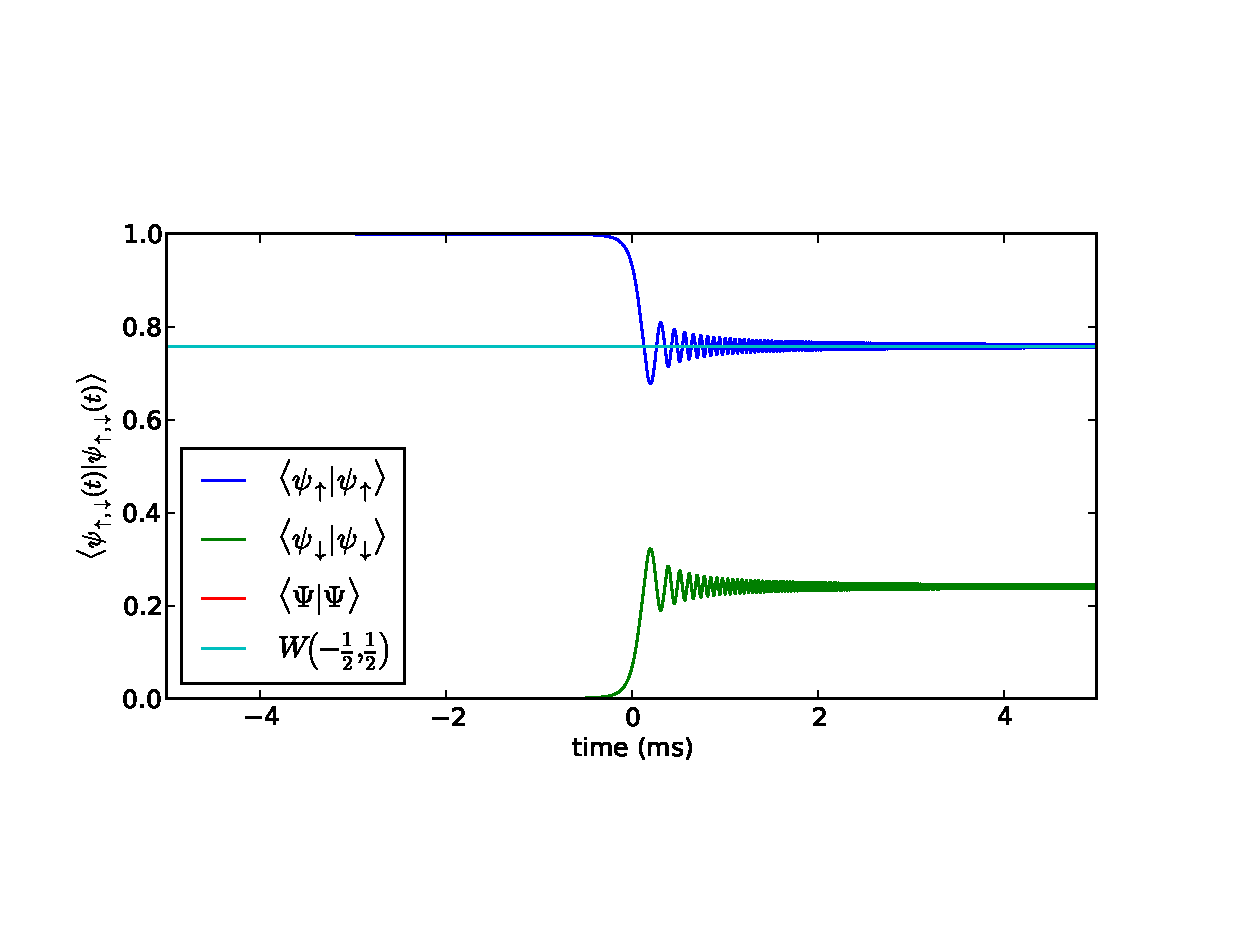
\includegraphics[width=0.75\textwidth]{gfx/Ehrenfest/labframeFlip}}\quad
\subfloat[Rotating frame flip]{\label{fig:rotframeFlip}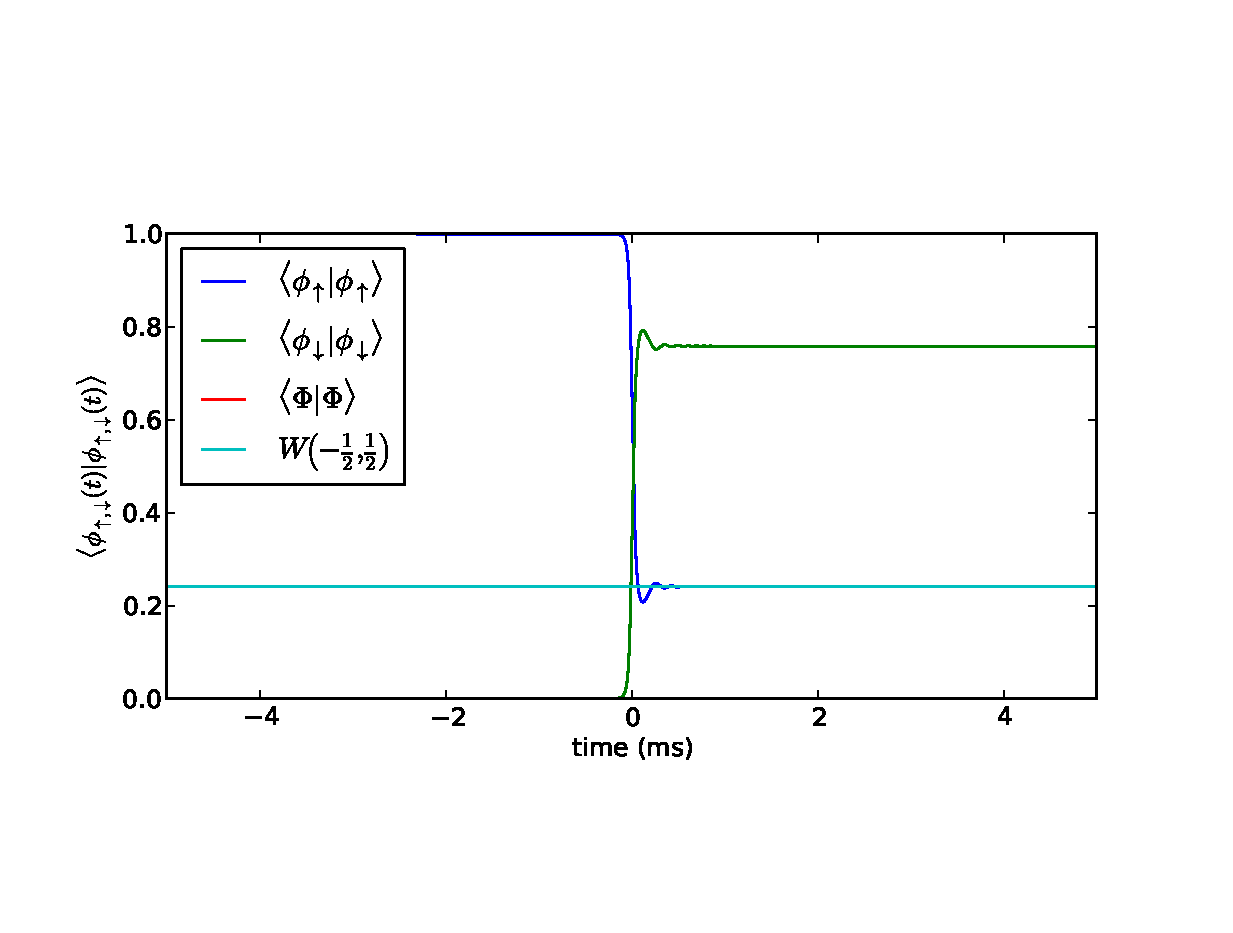
\includegraphics[width=0.75\textwidth]{gfx/Ehrenfest/rotframeFlip}}
}\\\_
\hspace{-6em}
\makebox[1.8\linewidth][l]{%
\centering
\subfloat[Lab frame no flip, $B_t=2\times10^{-7}$]{\label{fig:labframeNoFlip}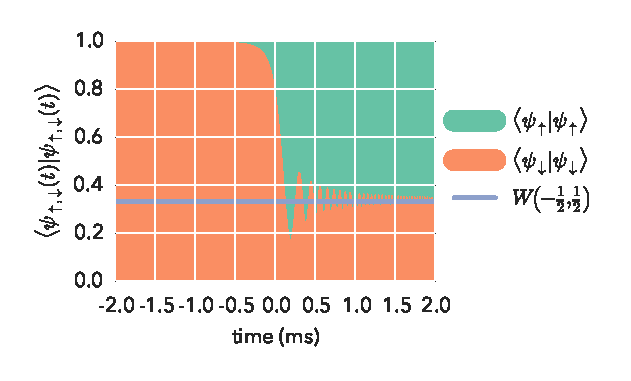
\includegraphics[width=0.75\textwidth]{gfx/Ehrenfest/labframeNoFlip}}\quad
\subfloat[Rotating frame no flip]{\label{fig:rotframeNoFlip}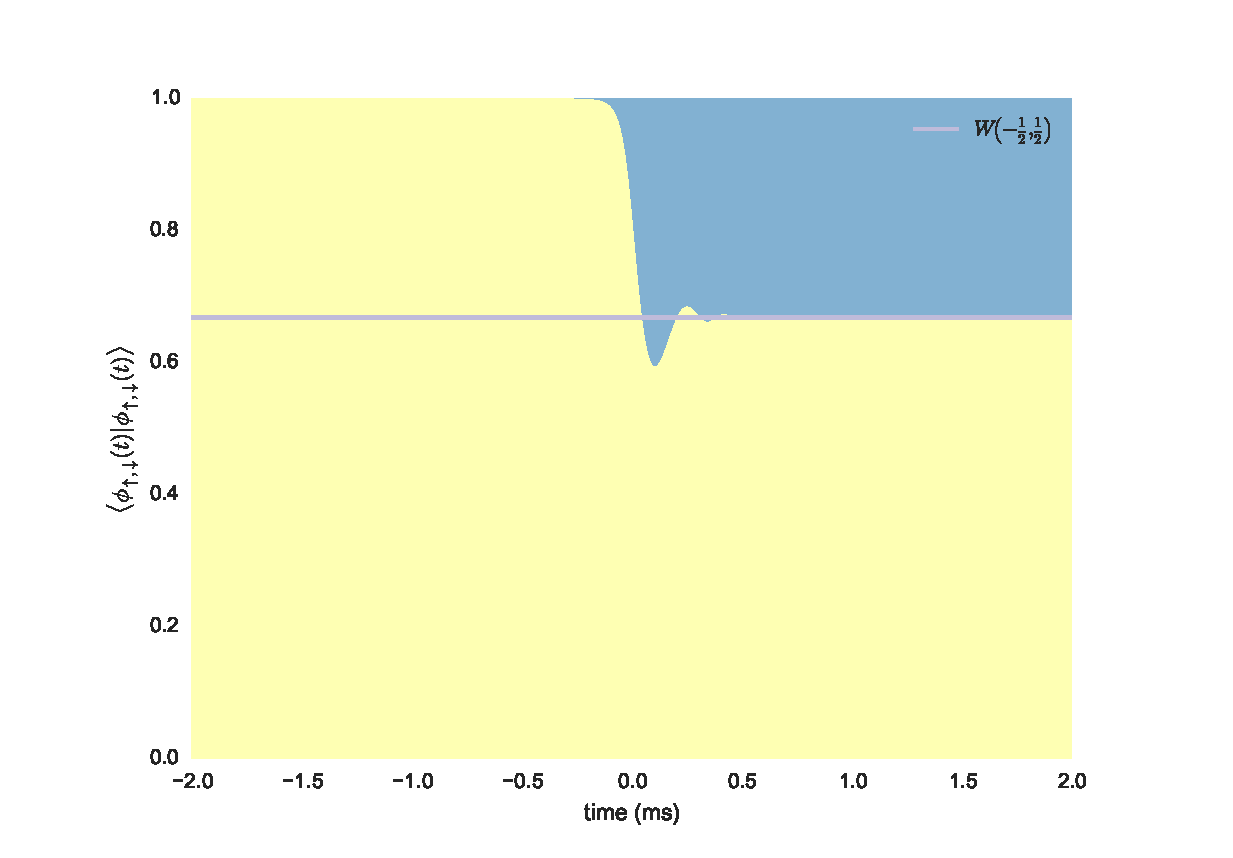
\includegraphics[width=0.75\textwidth]{gfx/Ehrenfest/rotframeNoFlip}}
}
\caption{Simulating the no majorana spin flip }\label{fig:majprob}
\end{figure}

Figures \ref{fig:labframeFlip} and \ref{fig:rotframeFlip} both illustrate a Majorana spin flip.
In this simulation we used the magnetic field $\mathbf{B}=(0.1,0.0,2500t)\,\mathrm{mT}$, and began at $t=-15\,\mathrm{ms}$ where the population in the spin component in the lab frame is less than $10^6$ (although we have plotted a smaller time window in figure \ref{fig:majprob}).
We can see the distinct different between the behaviour of the spin populations in the two different reference frames.
The initial wavefunction was chosen such that the population of the spin up component in the lab frame was 1.
Figure \ref{fig:rotframeFlip} clearly displays a change in the most probable state, whereas in figure \ref{fig:labframeFlip} it is not so clear.
Again this is because in the lab frame the spin up direction changes at $t=0$ when the sign of the $z$ component of the magnetic field moves from negative to positive.
Figures \ref{fig:labframeNoFlip} and \ref{fig:rotframeNoFlip} results from a simulation with $\mathbf{B}=(0.2,0.0,2500t)\,\mathrm{mT}$.
In these plots we see the converse behaviour in the state populations, indicating that no spin flip has occurred.

For both simulations we have used a time step of $\Delta t = 1\,\mu\mathrm{s}$.
This may seem overkill given the rate of change of the magnetic field can be characterised by $\tau_B=\vert\mathbf{B}\vert / \partial_t\vert\mathbf{B}\vert = 15\,\mathrm{ms}$ at the beginning of the simulation.
However there is another time scale that must be considered in a simulation like this, that is the period of a Larmor precession, $T_L = 2\pi\hbar / g_s \mu_B \vert\mathbf{B}\vert = 3.81\,\mu\mathrm{s}$ at the begining of the simulation.
While we do not expect the spin to precess for the first half of the simulation when it is completely aligned with the magnetic field, it is the period close to the field minimum and beyond that will experience Larmor precession.
In fact the wiggles after the spin flip occur at the Larmor precision frequency.
For example, look at one period of oscillation around $t=0.3\,\mathrm{ms}$, here the Larmor precession period will be, $T_L=0.19\,\mathrm{ms}$, exactly as simulated (**MAKE INSET IN FIGURE TO SHOW LARMOR PRECESSION RATE**).

\marginpar{The astute reader may be confused by line 4 of the pseudo-code in listing \ref{lst:Ehrenfest}.
The appearance of the $n+1^\mathrm{th}$ velocity when calculating the $n+1^\mathrm{th}$ position is not how one might implement the standard Euler integration method. 
Here we have used an implementation of the Symplectic Euler method \cite{??}, which has better energy conserving properties than the standard forward Euler.
This technique still has the same order accuracy with time, and introduces no added computational complexity, yet we gain some extra stability in the total energy of the atom.}

%------------------------------------------------

\section{Single Atom Spin Flips}

Confident in our ability to accurately simulate the Schr\"odinger equation, in our regime of interest, we may begin to apply the Ehrenfest method to simulating spin flips of real atoms.
The first step is to first see wether or not we can simulate the spin flip of a single atom.
I have given a pseudo-code example for a single time step of the Ehrenfest algorithm in listing \ref{lst:Ehrenfest}\footnote{Note in listing \ref{lst:Ehrenfest} that we have denoted the discrete approximation to a continuous variable as, $g_n \approx g(t_n)$.}.
\begin{lstlisting}[float,caption=Psuedo-code algorithm for a single Ehrenfest method time step, mathescape,label= lst:Ehrenfest,stepnumber=1]
Calculate force using current spin state: $\mathbf{F}_n = \bra{\Psi_n}\widehat{\mathbf{F}}_n\ket{\Psi_n}$.
Evolve wavefunction using time evolution operator: $\ket{\Psi_{n+1}} = \widehat{U}_n \ket{\Psi_{n}}$.
Evolve velocity using the average force: $\mathbf{v}_{n+1} = \mathbf{v}_n + \mathbf{F}_n \Delta t / m$.
Evolve position using the new velocity: $\mathbf{x}_{n+1} = \mathbf{x}_n + \mathbf{v}_{n+1} \Delta t$.
\end{lstlisting}

\begin{figure}
\hspace{-8em}
\makebox[1.8\linewidth][l]{%
\centering
\subfloat[Co-rotating frame spins]{\label{fig:ehrenfestSpin}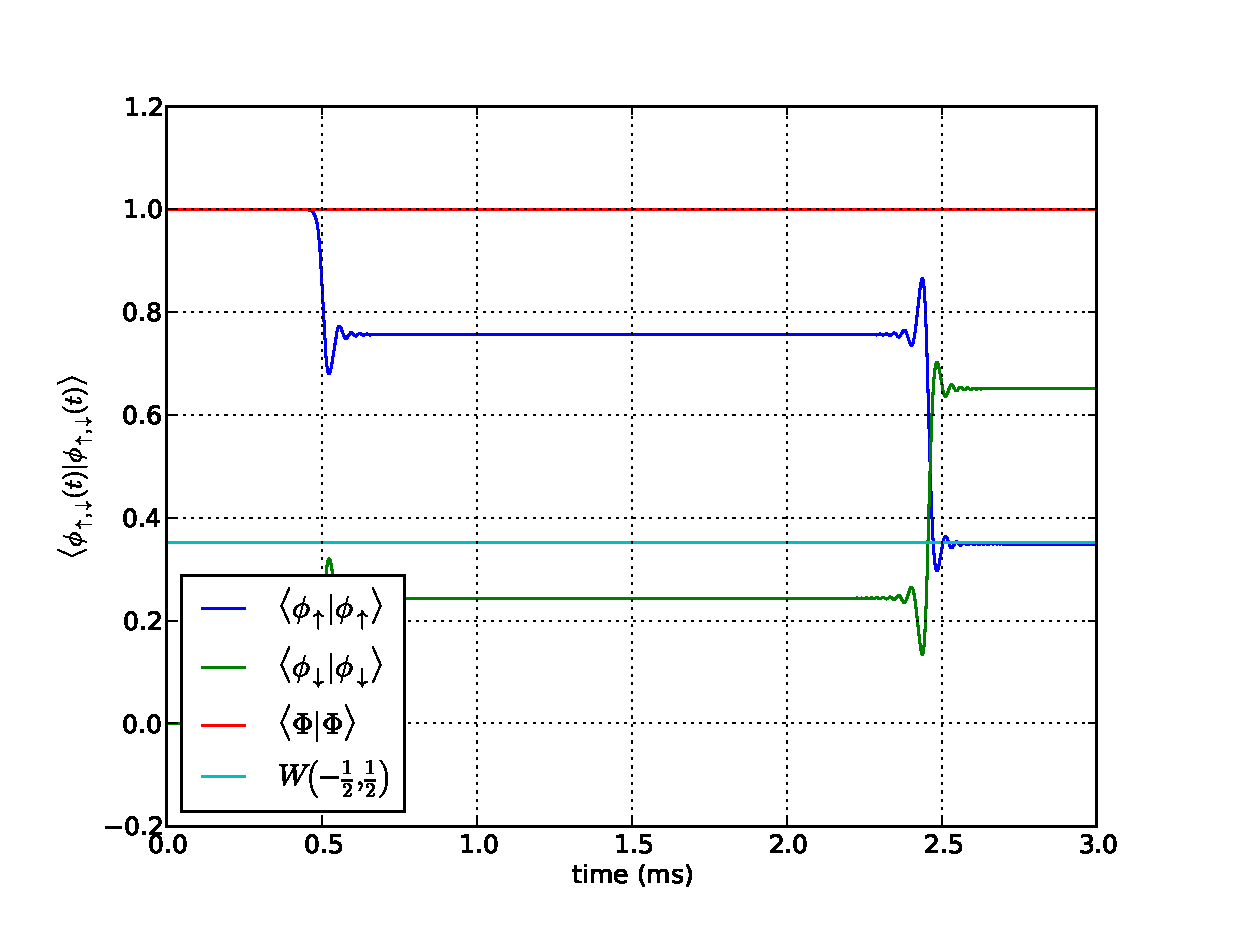
\includegraphics[width=0.525\textwidth]{gfx/Ehrenfest/ehrenfestSpin}}\quad
\subfloat[Position and velocity]{\label{fig:ehrenfestPos}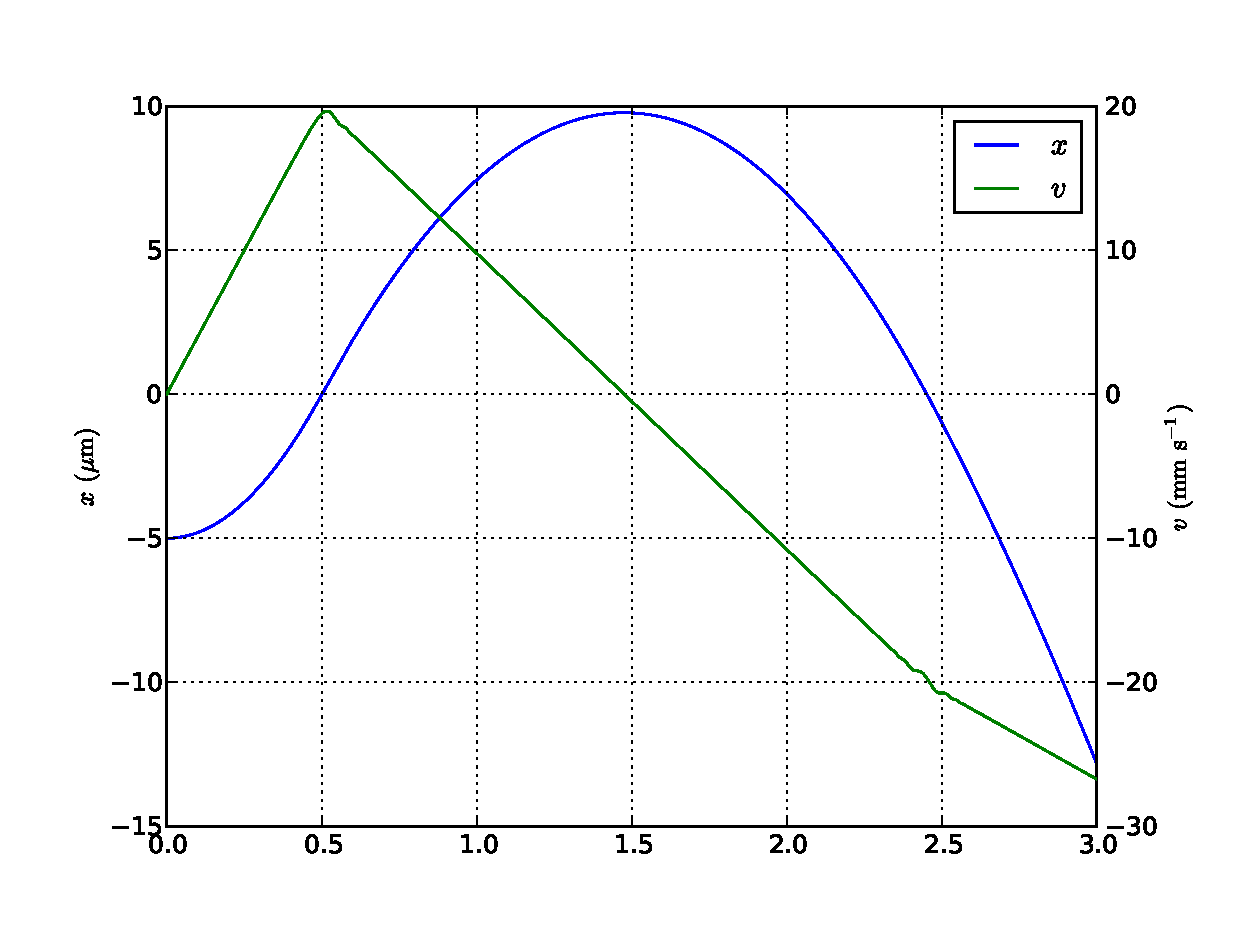
\includegraphics[width=0.525\textwidth]{gfx/Ehrenfest/ehrenfestPos}}\quad
\subfloat[Energy]{\label{fig:ehrenfestEnergy}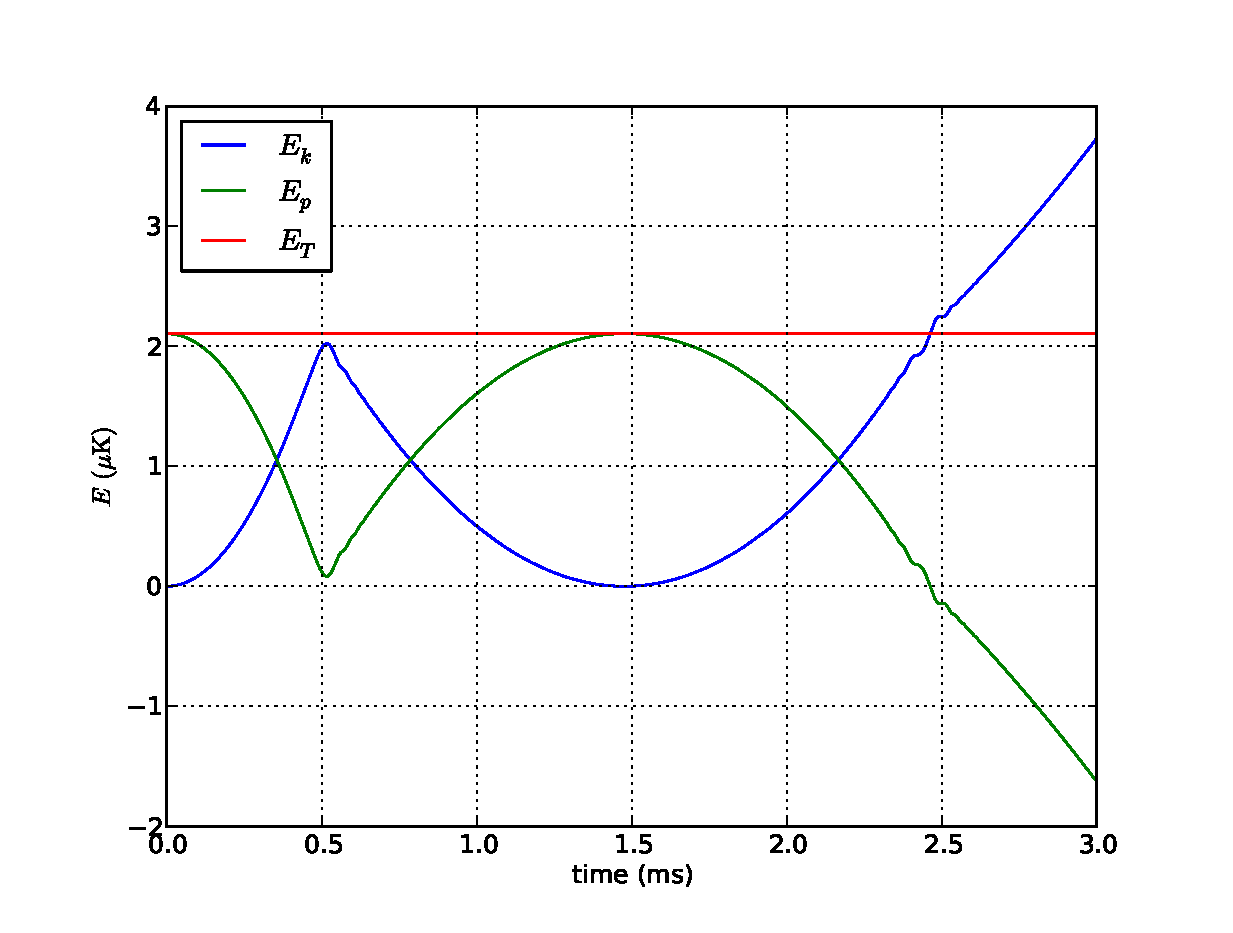
\includegraphics[width=0.525\textwidth]{gfx/Ehrenfest/ehrenfestEnergy}}%
}
\caption{No flip and flip in the same simulation.}\label{fig:ehrenfestFlip}
\end{figure}

Figure \ref{fig:ehrenfestFlip} shows the results from one such simulation.
This simulation was of a rubidium 87 atom the began at $x=-5\,\mu\mathrm{m}$ with a zero initial velocity.
Again the initial wavefunction was chosen so that it would be completely spin up in the co-rotating frame.
The magnetic field was given by $\mathbf{B} = (B_x,0,B_z'z)$, with $B_z=1\,\mu\mathrm{T}$ and $B_z'=2.5\,\mathrm{Tm}^{-1}$\footnote{I am aware that this magnetic field does not satisfy Maxwell's equations, but it serves as a nice example and more closely aligns with the field considered by Majorana.}.
This is a fabulous example of how well the Ehrenfest method can work.
Figure \ref{fig:ehrenfestSpin} displays how well the spin populations are simulated.
Again they agree with the predictions of the Majorana formula and the total probability is conserved.
\marginpar{Say how I can still use the Majorana formula here. $c =v(t=0) B_z'$.}
In figure \ref{fig:ehrenfestPos} I have plotted the position and velocity of the atom as it moves through time.
We can see how the atom remains trapped after the first partial flip and is then completely ejected from the trapped once it has flipped.
Finally figure \ref{fig:ehrenfestEnergy} shows how the total energy of the atom is conserved throughout the simulation (even after is has flipped).
So things seem to be working quite well, but earlier I alluded to the fact that the Ehrenfest method is not suitable to this kind of problem, so what is wrong?
I will let you stew on this few a few sections while we investigate the behaviour of a full gas simulation.

%----------------------------------------------------------------------------------------

\section{Full Gas Simulations}

Convinced that our Ehrenfest method can simulate spin flips and conserves both energy and probability we can begin to run some full gas simulations.
Majorana spin flips only occur when there is a sharp transition in magnetic field direction, like that transition that is present around the centre of a quadrupole trap.
An IP trap does not have this kind of transition, thus we would expect a very small number (~0) of spin flips to occur as a result of the IP field configuration.
As a cautionary test we will simulate a gas trapped in an IP trap using the Ehrenfest method.

%------------------------------------------------

\subsection{Ioffe Pritchard Trap}

The IP trap will remove any of the complex dynamics (and atom loss) we would experience from Majorana loss.
This will allow us to simulate the energy and probability conserving characteristics of the method, as well as ensure that the simulated particle dynamics are as expected.

\begin{figure}
\hspace{-11em}
\makebox[1.8\linewidth][l]{%
\centering
\subfloat[IP Distribution]{\label{fig:ehrenfestIPDist}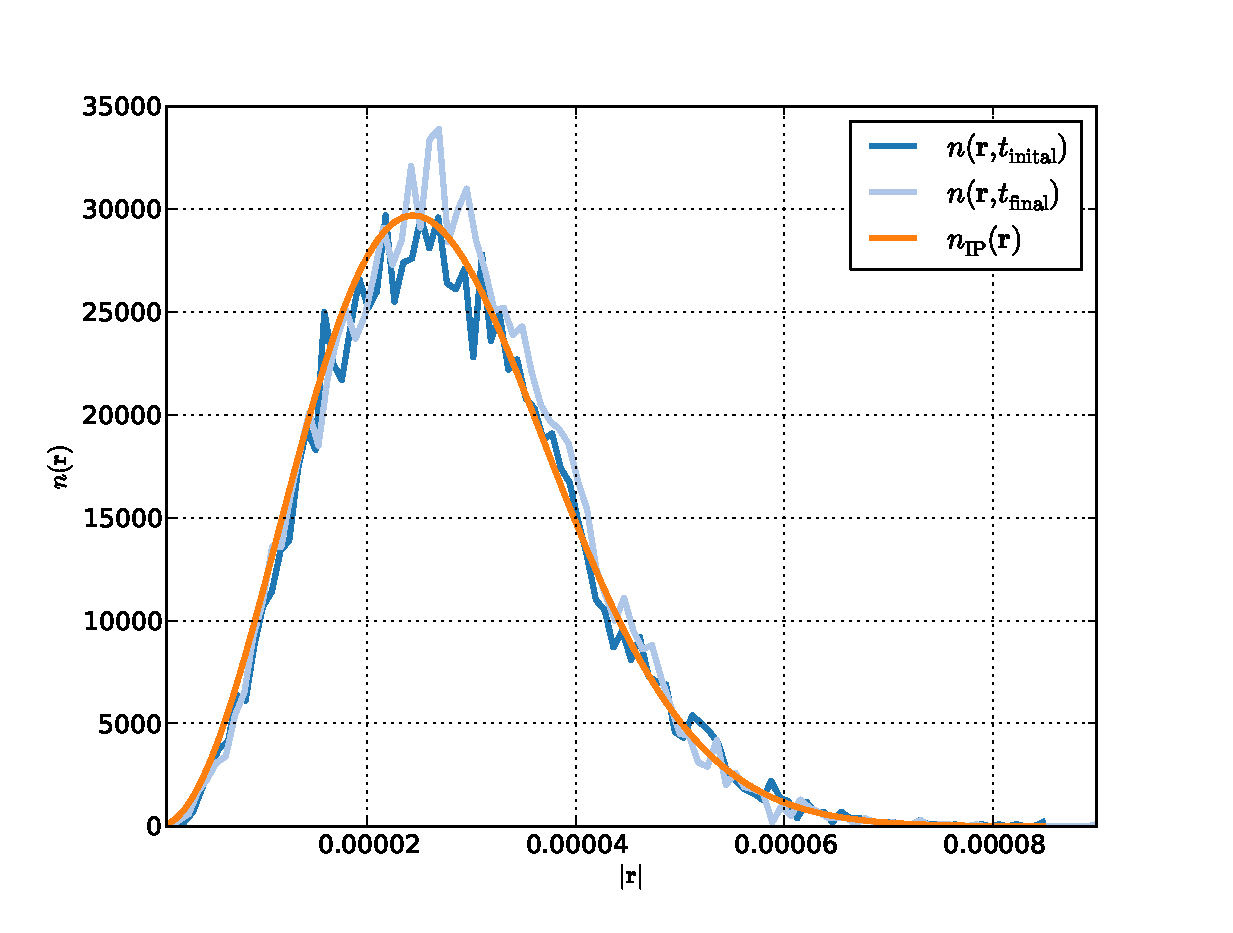
\includegraphics[width=0.75\textwidth]{gfx/Ehrenfest/ehrenfestIPDist}}\quad
\subfloat[IP Conservation]{\label{fig:ehrenfestIPCons}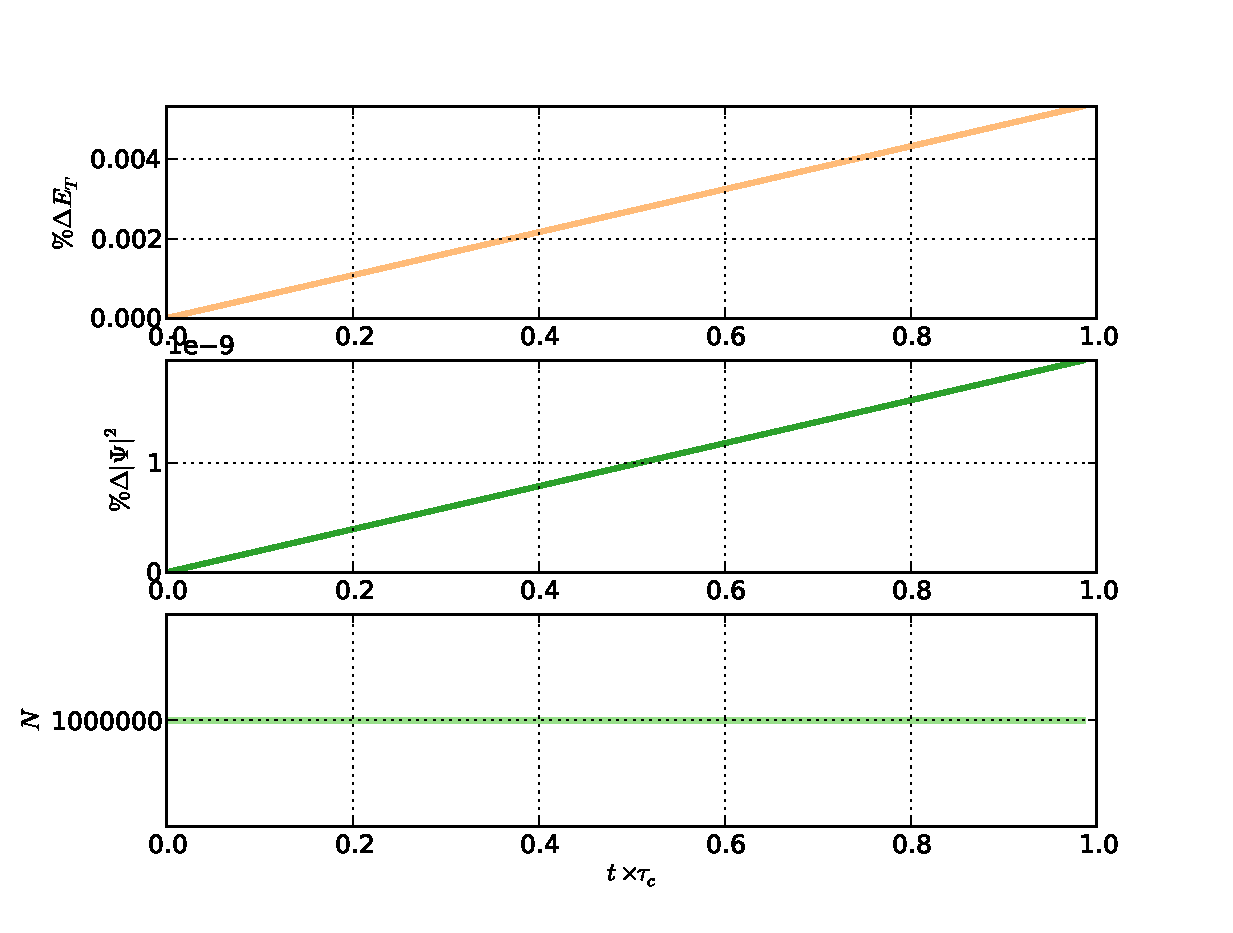
\includegraphics[width=0.75\textwidth]{gfx/Ehrenfest/ehrenfestIPConserve}}
}
\caption{Ehrenfest method for a gas in an IP trap.}\label{fig:ehrenfestIP}
\end{figure}

The results from a simulation of $10^6$ rubidium 87 atoms at $2\,\mu\mathrm{K}$ in an IP with $B_0=0.01\,\mathrm{T}$, $B'=20.0\,\mathrm{Tm}^{-1}$ and $B''=40,000\,\mathrm{Tm}^{-2}$ over a period of approximately 10 collision times ($10\tau_c$) are shown in figure \ref{fig:ehrenfestIP}.
In this figure I have tried to show the conservative properties of the Ehrenfest method.
Figure \ref{fig:ehrenfestIPDist} illustrates the radial distribution of particles.
I have drawn the distribution at the beginning and the end of the simulation, as well as contrast it with the analytic result for a thermal gas.
\marginpar{The density distribution for a thermal gas is $n(\mathbf{r}) = n_0 \exp\left[-\mathcal{U}(\mathbf{r})/k_BT\right]$.}
As we can see the numerical result is very stable and agrees well with the analytic prediction.
In figure \ref{fig:ehrenfestIPCons} I have illustrated the change in the quantities we would expect to be conserved in a simulation like this.
The top graph shows the percentage change in the average total energy, the middle graph shows the percentage change in the average norm of the wavefunction and the bottom graph shows the number of atoms.

First of all we can note there is no change in the number of atoms \ie no Majorana spin flips.
This simulation has the same evaportaion code running as we developed in section \ref{sec:evaporation}, with the evaporation condition that if $P_z < 0$ the atom is removed.
This is due to the presence of the non-zero field bias, $B_0$, which ensures that the Larmor precession rate is always greater than the rate of change of the magnetic field direction.
Second we can see a linear increase in the total energy and wavefunction norm.
How can this be, I thought we were using fancy symplectic methods that were designed to conserve these quantities.
I have two responses to that question, the first is can we really call a \%0.005 (that is 1 in 20,000) increase a significant change?
For the simulation I have run here this corresponds to the total energy changing by $0.3\,\mathrm{nK}$, not we might consider a significant increase in temperature.
However, we can argue that there is a clear linear trend and if we anticipate running extended simulations this might be something that we wish to keep in mind.
Although I wouldn't consider this deal breaker.
My second response would be that the time step I have used is far too large.
For this simulation I have used the time step, $\Delta t = 5\,\mathrm{ns}$.
This might seem quite small but compared to the Larmor period at the the average radius, $T_L\approx 10^{-8}\,\mathrm{s}$, it isn't that great.
Not only does this mean on average we are only sampling the wavefunction twice per Larmor rotation, but out on the edges of the gas we are doing far worse!
Of course we could reduce the time step, and this would improve our energy conservation, but to be able to run these simulations in a reasonable time frame we must accept a certain level of non-conservation in our total energy and wavefunction norm.

Overall this seems to have worked quite well and yet I keep saying that the Ehrenfest method is not suitable for our simulations.
Let's now try to run a simulation in a quadrupole trap and see how effective the method is.
%------------------------------------------------

\subsection{Quadrupole Trap}

Content % DSMC WITH SPIN - EHRENFEST
% Chapter X

\chapter{DSMC WITH SPIN - MCWF} % Chapter title

\label{ch:dsmcmcwf} % For referencing the chapter elsewhere, use \autoref{ch:dsmcmcwf} 

I guess I need to talk about the MCWF method here, this could be difficult.

%---------------------------------------------------------------------------------------
\section{Single Atom Spin Flips}

Just like we did with the Ehrenfest method in section \ref{sec:EhrenfestSingleAtom} we can begin by simulating the a spin flip of a single atom in a Majorana type trap. 
To make the comparison between the two methods fair we will again use the same magnetic field, $\mathbf{B} = (B_x,0,B_z'z)$, with $B_x=1\,\mu\mathrm{T}$ and $B_z'=2.5\,\mathrm{Tm}^{-1}$.
Our rubidium 87 atom will also have the same initial conditions, $z=-5\,\mu\mathrm{m}$ and zero initial velocity, $v_z=0\,\mathrm{ms}^{-1}$.
Finally we will use the same simulation time step, $\Delta t = 0.1\,\mu\mathrm{s}$.
The only difference here is that we must average the result over a large number of simulations, in this case we have run $10^5$ independent simulations.

\begin{figure}
\hspace{-8em}
\makebox[1.8\linewidth][l]{%
\centering
\subfloat[Co-rotating frame spins]{\label{fig:mcwfMajoranaSpin}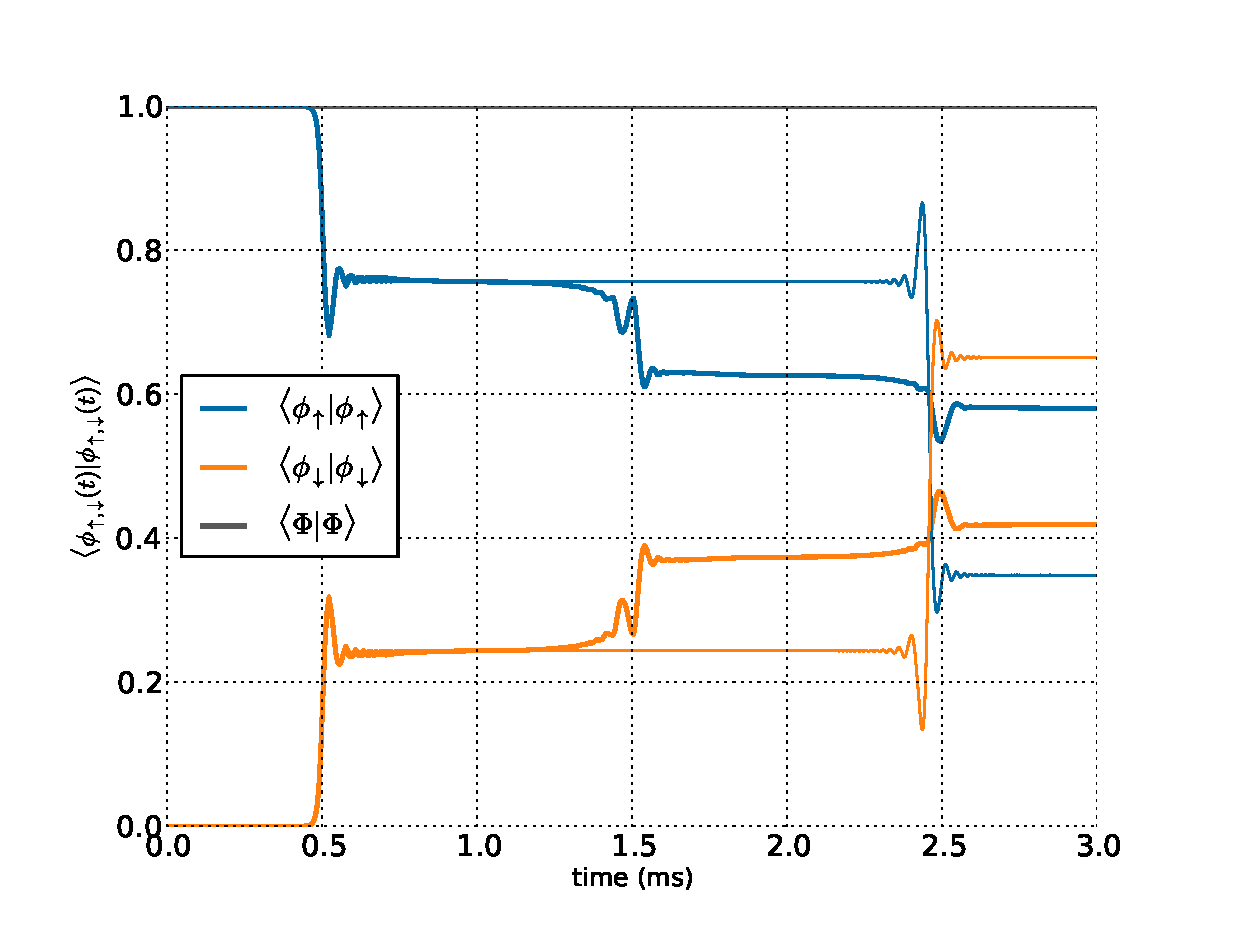
\includegraphics[width=0.525\textwidth]{gfx/MCWF/mcwfMajoranaSpin}}\quad
\subfloat[Position and velocity]{\label{fig:mcwfMajoranaTrajectory}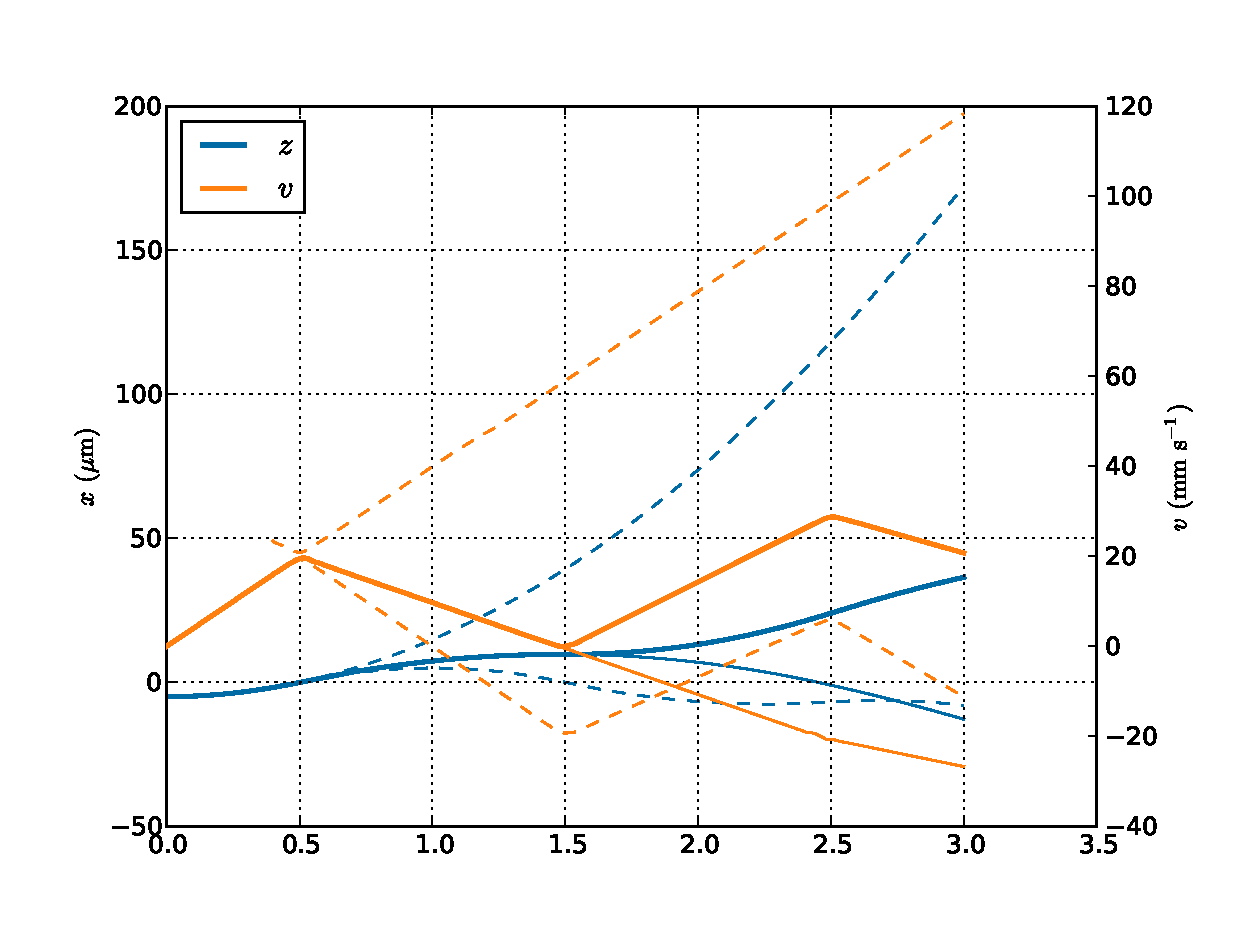
\includegraphics[width=0.525\textwidth]{gfx/MCWF/mcwfMajoranaTrajectory}}\quad
\subfloat[Energy]{\label{fig:mcwfMajoranaEnergy}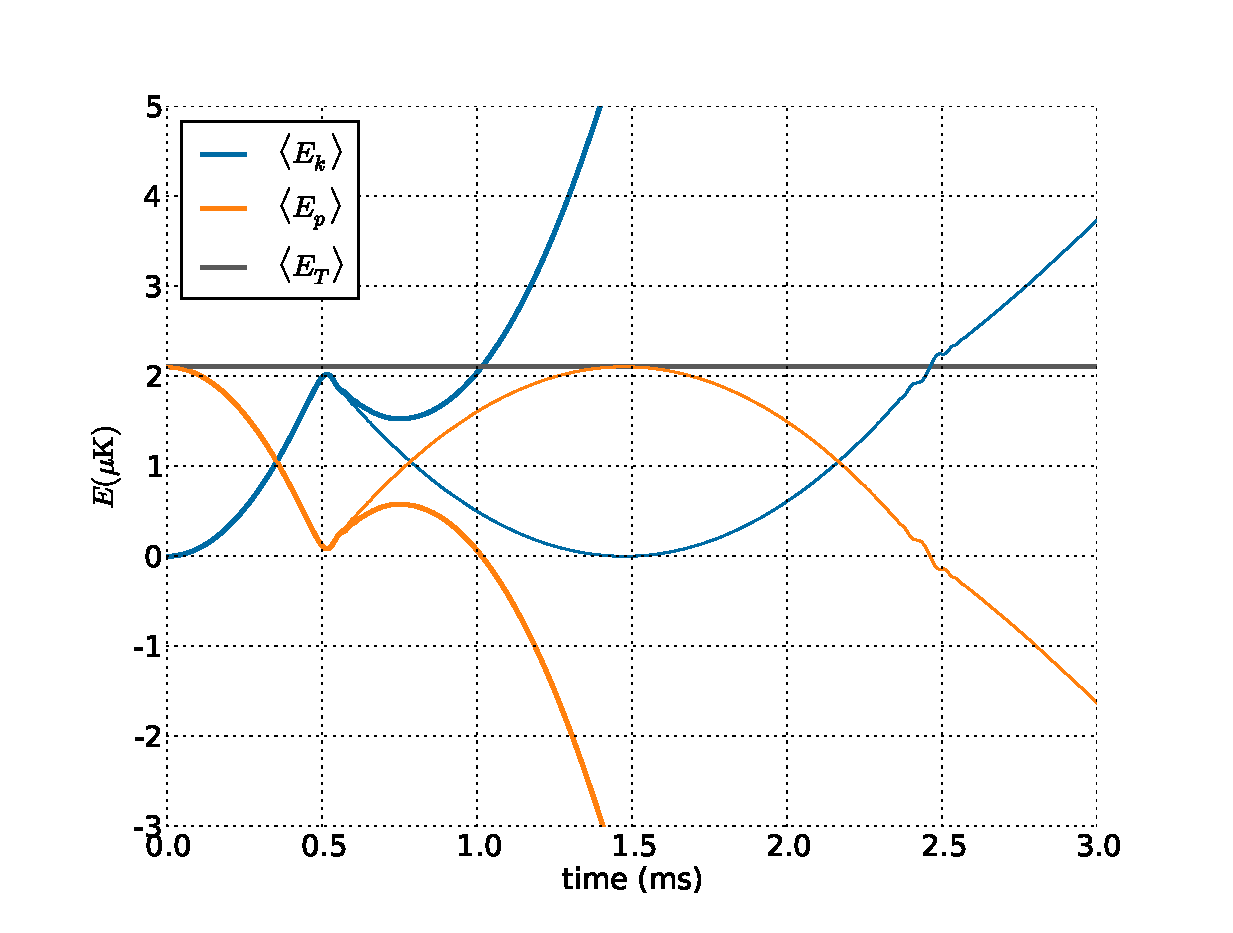
\includegraphics[width=0.525\textwidth]{gfx/MCWF/mcwfMajoranaEnergy}}%
}
\caption{No flip and flip in the same simulation mcwf.}\label{fig:mcwfFlip}
\end{figure}

At last, in figure \ref{fig:mcwfFlip} we have some convincing proof of the failure of the Ehrenfest method.
First let's get the boring stuff out of the way.
Figure \ref{fig:mcwfMajoranaSpin} illustrates that the MCWF method conserves probability, similarly figure \ref{fig:mcwfMajoranaEnergy} shows the energy conservation of the method.
Now let's compare the differences between the Ehrenfest and MCWF methods.
We'll start by comparing the wavefunction evolution depicted in figure \ref{fig:mcwfMajoranaSpin}.
Here we see the two methods agree perfectly for the first magnetic field minimum crossing.
However, at around $1.5\,\mathrm{ms}$ we see the MCWF method make, what looks to be another spin flip, and then another at $2.5\,\mathrm{ms}$.
How can this be?
What is it that causes the particles in the MCWF method to experience an extra spin flip?
This questions is most clearly illustrated in figure \ref{fig:mcwfMajoranaTrajectory}.
The bold lines indicate the averaged trajectories of the MCWF particles.
Again up until the $1.5\,\mathrm{ms}$ mark the two approaches (Ehrenfest and MCWF) agree exactly.
So what is it that happens at $1.5\,\mathrm{ms}$ that causes this deviation?
Consider the trajectories shown by the dashed lines.
These lines represent the average trajectories of all the particles who are considered to be in a trapped state.
Conversely the dash-dotted lines are the untapped state.
While the average of these two trajectories produces the same result as the Ehrenfest method (as we might expect), the physical path taken by the particles is completely different.
So the reason for the apparent extra spin flip at $1.5\,\mathrm{ms}$ is due to the extra crossing of the field minimum experienced by the particles that remain in the trapped state.
So what happens in the Ehrenfest simulation?
What is it that produces its failure?
The Ehrenfest method will move particle along the trajectory described by the average force.
At $0.5\,\mathrm{ms}$ after the first crossing of the field minimum the particle experiences a partial flip.
Since the particle is moved with the average force the trapping force of the particle is now weaker and it is effectively trapped in a looser magnetic field.
While on average this may be a reasonable way to think about the problem, we have already seen that it does not produce the correct dynamics for particles moving in a simple one-dimensional trap.

How does this result explain the disagreement of the Ehrenfest method with the test done in section \ref{sec:EhrenfestQuad}?
When a particle experiences a partial flip the Ehrenfest method will then subject it to a weaker trapping force, essentially loosening or widening the trapping potential.
So in figure \ref{fig?} as the particles of the gas slowly begin to tip over, from the cumulative effect of many partial flips, the gas begins to unnaturally widen.
As a result the calculated temperature is higher than what one would physically expect.
In practice we know that an atom is either in a trapped state or an untrapped state (not partially in both).
So a real trapped gas that is subjected to Majorana spin flips should not display a widening due to the weakening trapping potential, it should only exhibit atom loss due to the fully flipped atoms leaving the trap\footnote{Of course this will also result in a widening of the trap due to the heating effect cause by the selective removal of the least energetic particles.}.

So why does the Ehrenfest method seem to work for the Ioffe Pritchard trap?
We do not expect atoms in the IP trap to undergo any kind of spin flip.
The geometry of the trap is such that the rate of change of the magnetic field direction is always (JUSTIFY?) less than the Larmor precession rate.
So the particles in the simulation shown in figure \ref{fig:ehrenfestIP} are always subjected to the full trapping potential.

%----------------------------------------------------------------------------------------

\section{Full Gas Simulations}

Content

%------------------------------------------------

\subsection{Ioffe Pritchard Trap}

Content

%------------------------------------------------

\subsection{Quadrupole Trap}

Content % DSMC WITH SPIN - MCWF

\cleardoublepage % Empty page before the start of the next part

%----------------------------------------------------------------------------------------
%	THESIS CONTENT - FEMDVR
%----------------------------------------------------------------------------------------

\ctparttext{You can put some informational part preamble text here. Illo principalmente su nos. Non message \emph{occidental} angloromanic da. Debitas effortio simplificate sia se, auxiliar summarios da que, se avantiate publicationes via. Pan in terra summarios, capital interlingua se que. Al via multo esser specimen, campo responder que da. Le usate medical addresses pro, europa origine sanctificate nos se.} % Text on the Part 1 page describing  the content in Part 1

\part{FEMDVR} % First part of the thesis

% Chapter X

\chapter{CUDA FEMDVR} % Chapter title

\label{ch:name} % For referencing the chapter elsewhere, use \autoref{ch:name} 

%----------------------------------------------------------------------------------------

\section{1D FEMDVR}

Content

%------------------------------------------------

\subsection{Scaling Comparison to CPU}

Content

%------------------------------------------------

\subsection{Real Simulation}

Content

%----------------------------------------------------------------------------------------

\section{3D FEMDVR}

Content

%------------------------------------------------

\subsection{Knots}

Content % Chapter 4 - blank template

\cleardoublepage % Empty page before the start of the next part

%------------------------------------------------

%----------------------------------------------------------------------------------------
%	THESIS CONTENT - CUDA
%----------------------------------------------------------------------------------------

\ctparttext{You can put some informational part preamble text here. Illo principalmente su nos. Non message \emph{occidental} angloromanic da. Debitas effortio simplificate sia se, auxiliar summarios da que, se avantiate publicationes via. Pan in terra summarios, capital interlingua se que. Al via multo esser specimen, campo responder que da. Le usate medical addresses pro, europa origine sanctificate nos se.} % Text on the Part 1 page describing  the content in Part 1

\part{CUDA} % First part of the thesis

% Chapter CUDADSMC

\chapter{CUDA DSMC} % Chapter title

\label{ch:cudadsmc} % For referencing the chapter elsewhere, use \autoref{ch:name} 

%----------------------------------------------------------------------------------------

\section{CUDA}

Content

%------------------------------------------------

\subsection{Parallelisation}

Content

%----------------------------------------------------------------------------------------

\section{Speed up}

Content

%------------------------------------------------

\subsection{Some simulations}

Content % Chapter 4 - blank template

\cleardoublepage % Empty page before the start of the next part

%------------------------------------------------

%----------------------------------------------------------------------------------------
%	THESIS CONTENT - APPENDICES
%----------------------------------------------------------------------------------------

\appendix

\part{Appendix} % New part of the thesis for the appendix

%Appendix Motion Integration 

\chapter{ Thermal Physics } \label{app:thermalPhysics}

\section{Collision Rates in Thermal Gases} \label{app:collisionRates}

\section{ Thermalisation } \label{app:thermalisation}

\subsection{ Walraven Thermalisation } \label{app:walravenTherm}

 %Appendix ? - Thermal Physics stuff -- collision rates etc.
%Appendix Motion Integration 

\chapter{ Magnetic Trapping } \label{sec:magneticTrapping} % Appendix ? - magnetic trapping
%Appendix Motion Integration 

\chapter{ Motion Integration }

%--------------------------------------------------------------------------

In this appendix we will explain in detail the different methods of integrating the Newtonian motion of particles and specifically how we have gone about it.

\section{ Euler Method }

\begin{align}
    x_{n+1} &= x_{n} + v_{n} \Delta t,\\
    v_{n+1} &= v_{n} + a_{n} \Delta t.
\end{align}

%--------------------------------------------------------------------------

\section{ Semi-Implicit Euler Method }

\begin{align}
    x_{n+1} &= x_{n} + v_{n} \Delta t,\\
    v_{n+1} &= v_{n} + a_{n+1} \Delta t.
\end{align}


%--------------------------------------------------------------------------

\section{ Verlet Algorithm }

Sometimes referred to as the St\"ormer-Verlet method (see wikipedia page it's pretty good), it was made popular by Verlet in 1976 \cite{Verlet1967}. The Verlet algorithm can be derived from the Taylor series expansions for position as follows,
\begin{subequations}
\begin{align}
    \mathbf{r}(t_{n+1}) &= \mathbf{r}(t_{n}) + k \mathbf{v}( t_{n} ) + \frac{1}{2}k^2\mathbf{a}(t_{n}) + {\mathcal O}(k^3), \label{eq:TaylorPlus}\\
    \mathbf{r}(t_{n-1}) &= \mathbf{r}(t_{n}) - k \mathbf{v}( t_{n} ) + \frac{1}{2}k^2\mathbf{a}(t_{n}) + {\mathcal O}(k^3),\label{eq:TaylorMinus}
\end{align}
\end{subequations}
we can now add equations \eqref{eq:TaylorPlus} and \eqref{eq:TaylorMinus} together to get
\begin{align}
    \mathbf{r}(t_{n+1}) + \mathbf{r}(t_{n-1}) &= 2\mathbf{r}(t_{n}) + k^2\mathbf{a}(t_{n}) + {\mathcal O}(k^4),\notag\\
    \Rightarrow \mathbf{r}(t_{n+1}) &= 2\mathbf{r}(t_{n}) - \mathbf{r}(t_{n-1}) + k^2\mathbf{a}(t_{n}) + {\mathcal O}(k^4),\label{eq:LeapFrog}.
\end{align}
We can see from equation \eqref{eq:LeapFrog} that the leap frog method is fourth order in time. However, we can also note that the velocities do not explicitly appear in the method, this means we need to derive them from positions. A simple approximation would be to use the midpoint method
\begin{equation}
    \mathbf{v}(t_{n}) = \frac{1}{2}k\left(\mathbf{r}(t_{n+1}) - \mathbf{r}(t_{n-1})\right)
\end{equation}


%--------------------------------------------------------------------------

\section{ Leap Frog Method }

\cite{Hockney1970}

\begin{align}
    x_{n} &= x_{n-1} + v_{i-1/2} \Delta t,\\
    v_{n+1/2} &= v_{n-1/2} + a_{n} \Delta t.
\end{align}

%--------------------------------------------------------------------------

\section{ Velocity Verlet }

\cite{Swope1982}

\begin{align}
    x_{n+1} &= x_{n} + v_{i} \Delta t + \frac{1}{2} a_{n}{\Delta t}^2 ,\\
    v_{n+1} &= v_{n} + \frac{1}{2} \left( a_{n} + a_{n+1} \right) \Delta t.
\end{align}

%--------------------------------------------------------------------------

\section{ Beeman's Algorithm }

\cite{Beeman1976}

\begin{align}
    x_{n+1} &= x_{n} + v_{n} \Delta t + \frac{1}{6}\left( 4a_{n} - a_{n-1} \right) {\Delta t}^{2},\\
    v_{n+1} &= v_{n} + \frac{1}{6} \left( 2a_{n+1} + 5a_{n} - a_{n-1} \right) \Delta t.
\end{align}
 % Appendix ? - Motion Integration
% Appendix A

\chapter{Direct Simulation Monte Carlo}

%----------------------------------------------------------------------------------------

\lipsum[13-14]

%----------------------------------------------------------------------------------------

\section{Appendix Section Test}
\lipsum[15]

\graffito{More dummy text}
\lipsum[16]

%----------------------------------------------------------------------------------------

\section{Another Appendix Section Test}
\lipsum[17]

\begin{table}
\myfloatalign
\begin{tabularx}{\textwidth}{Xll} \toprule
\tableheadline{labitur bonorum pri no} & \tableheadline{que vista}
& \tableheadline{human} \\ \midrule
fastidii ea ius & germano &  demonstratea \\
suscipit instructior & titulo & personas \\
\midrule
quaestio philosophia & facto & demonstrated \\
\bottomrule
\end{tabularx}
\caption[Autem usu id]{Autem usu id.}
\label{tab:moreexample}
\end{table}

\lipsum[18]

\begin{lstlisting}[float,caption=A floating example]
for i:=maxint to 0 do
begin
{ do nothing }
end;
\end{lstlisting} % Appendix A - Direct Simulation Monte Carlo
% Appendix B

\chapter{Non-Dimensionalisation}

%----------------------------------------------------------------------------------------

\section{Quasi - 1D GPE}

Let's just start with writing out the full quasi-one-dimensional three component equation in a harmonic potential
\begin{subequations}
    \begin{align}
        \imath\hbar\frac{\partial}{\partial t} f_{+} &= \bigg(-\frac{\hbar^2}{2m}\frac{\partial^2}{\partial z^2} + \frac{1}{2}m{\omega_z}^2z^2+ E_+ + E_\perp + c_0 N\eta\rho \notag \\
        & \quad\quad\quad+ c_2 N\eta\left( \rho_+ + \rho_0 - \rho_- \right) \bigg)f_+ + c_2 N\eta{f_0}^2{f_-}^*,\label{eq:fplus}\\
        \imath\hbar\frac{\partial}{\partial t} f_{0} &= \bigg(-\frac{\hbar^2}{2m}\frac{\partial^2}{\partial z^2} + \frac{1}{2}m{\omega_z}^2z^2 + E_0 + E_\perp + c_0 N\eta\rho \notag \\
        & \quad\quad\quad+ c_2 N\eta\left( \rho_+ + \rho_- \right) \bigg)f_0 + 2c_2 N\eta{f_+}{f_-}{f_0}^*,\\
        \imath\hbar\frac{\partial}{\partial t} f_{-} &= \bigg(-\frac{\hbar^2}{2m}\frac{\partial^2}{\partial z^2} + \frac{1}{2}m{\omega_z}^2z^2 + E_- + E_\perp + c_0 N\eta\rho \notag \\
        & \quad\quad\quad+ c_2 N\eta\left( \rho_- + \rho_0 - \rho_+ \right) \bigg)f_- + c_2 N\eta{f_0}^2{f_+}^*,\\
        & \quad \rho\frac{\partial E_\perp}{\partial\chi} + \left(\frac{c_0 N}{2}\rho^2 + \frac{c_2 N}{2}S_2\right)\frac{\partial\eta}{\partial\chi} = 0. \label{rhoEqn}
    \end{align}
\end{subequations}
If we make the Thomas Fermi ansatz then the transverse mode energy and the scaling factor are given by
\begin{align}
    E_\perp &= \frac{\hbar\omega_\perp}{6}\frac{\chi^2}{{a_\perp}^2},\label{Eperp}\\
    \eta &= \frac{4}{3\pi\chi^2}, \label{eta}
\end{align}
where $a_\perp = \sqrt{\hbar / m\omega_\perp}$. If we substitute \eqref{Eperp} and \eqref{eta} into \eqref{rhoEqn} then we find
\begin{equation}
    \chi = \left(\frac{4 c_0 N \rho^2 + c_2 N S_2}{m\pi\rho{\omega_\perp}^2}\right)^{\frac{1}{4}}. \label{eq:chi}
\end{equation}
Now substituting \eqref{eq:chi} back into \eqref{Eperp} and \eqref{eta} and simplifying we have
\begin{align}
    E_\perp &= \sqrt{\frac{mN{\omega_\perp}^2 \left(c_0 \rho^2 + c_2 S_2\right)}{9\pi\rho}},\\
    \eta &= \frac{2}{3}\sqrt{\frac{m\rho{\omega_\perp}^2}{\pi N \left(c_0 \rho^2 + c_2 S_2\right)}}.
\end{align}
Now we can begin to non-dimensionalise the equations. Let us only consider the non-dimensionalisation of the positive component since the procedure will be exactly the same for all components. We begin by making the substitutions
\begin{align*}
    t &\to t_c \tau,\\
    z &\to z_c \zeta,\\
    f_+ &\to f_c u_+.
\end{align*}
Equation \eqref{eq:fplus} now becomes
\begin{align*}
    \imath\hbar\frac{f_c}{t_c}\frac{\partial}{\partial \tau} u_{+} &= \bigg(-\frac{\hbar^2}{2m{z_c}^2}\frac{\partial^2}{\partial \zeta^2} + \frac{1}{2}m{\omega_z}^2{z_c}^2\zeta^2 + f_c E_+ + f_c E_\perp + c_0 f_c N\eta\rho \notag \\
        &\quad \quad\quad + c_2 f_c N\eta\left( \rho_+ + \rho_0 - \rho_- \right) \bigg)f_c u_+ + c_2 {f_c}^2 N\eta{u_0}^2{u_-}^*,\\
    \imath\frac{m{z_c}^2}{\hbar t_c}\frac{\partial}{\partial \tau} u_{+} &= \bigg(-\frac{1}{2}\frac{\partial^2}{\partial \zeta^2} + \frac{1}{2}\frac{m^2{\omega_z}^2{z_c}^4}{\hbar^2}\zeta^2 + \frac{m{z_c}^2}{\hbar^2}f_c\big[E_+ + E_\perp + c_0  N\eta\rho \notag \\
        &\quad \quad\quad + c_2 N\eta\left( \rho_+ + \rho_0 - \rho_- \right) \big]\bigg) u_+ + \frac{m{z_c}^2}{\hbar^2} c_2 f_c N\eta{u_0}^2{u_-}^*.
\end{align*}
Looking at the coefficient of the $\zeta^2$ term we can see that if we set it to 1/2 we will be able to solve for $z_c$,
\begin{align}
    1 &= \frac{m^2 {w_z}^2 {z_c}^4}{\hbar^2},\notag\\
    \Rightarrow z_c &= \sqrt{\frac{\hbar}{m\omega_z}},
\end{align}
which is the harmonic oscillator length along the $z$ axis, a natural length scale for the $z$ dimension. Now we can turn our attention to the coefficient of the time derivative, and set it to $\imath$,
\begin{align}
    1 &= \frac{m{z_c}^2}{\hbar t_c},\notag\\
      &= \frac{m \hbar}{m \hbar \omega_z t_c},\notag\\
    \Rightarrow t_c &= \frac{1}{w_z},
\end{align}
which is the angular period of the oscillator, again a natural length scale. Finally we can consider the energy terms. With these we need to choose $f_c$ such that the dimension of the energy term is one. To cut a long story short, this makes a suitable choice for $f_c$ to be $1/\sqrt{z_c}$. Giving us the final form of the non-dimensionalised equation
\begin{align}
    \imath\frac{\partial}{\partial \tau} u_{+} &= \bigg(-\frac{1}{2}\frac{\partial^2}{\partial \zeta^2} + \frac{1}{2}\zeta^2 + \frac{m}{\hbar^2}\left(\frac{\hbar}{m\omega_z}\right)^{\frac{3}{4}}\big[E_+ + E_\perp + c_0  N\eta\rho \notag \\
        &\quad \quad\quad + c_2 N\eta\left( \rho_+ + \rho_0 - \rho_- \right) \big]\bigg) u_+ + \frac{m}{\hbar^2}\left(\frac{\hbar}{m\omega_z}\right)^{\frac{3}{4}} c_2 N\eta{u_0}^2{u_-}^*.
\end{align}



%----------------------------------------------------------------------------------------

\section{Majorana Problem Spin Half}
The potential energy operator \cite{foot:2005} for a magnetic dipole in a field is given by
\begin{equation}
    \hat{V} = -\hat{\boldsymbol\mu}\cdot\bf{B},
\end{equation}
where $\hat{\boldsymbol\mu}$ is the magnetic dipole operator and $\bf{B}$ is the magnetic field. Which for a spin half particle is 
\begin{equation*}
    \hat{V} = \frac{1}{2}\mu_{B}g_{s} \begin{bmatrix} B_{z}                & B_{x} - \imath B_{y} \\
                                                      B_{x} + \imath B_{y} & -B_{z} \end{bmatrix},
\end{equation*}
where $\mu_{B}$ is the Bohr magneton \cite{??} and $g_s$ is the Land\'e g-factor of the spin-$\frac{1}{2}$ particle. Now we can write the time dependant Schr\"odinger equation for our system (\textcolor{red}{need to introduce kinetic energy operator as well})
\begin{align}
    \imath \hbar \partial_t \psi_\uparrow &= -\frac{\hbar^{2}}{2m}\partial_{zz} \psi_\uparrow  + \frac{1}{2}\mu_{B}g_{s}B_{z} \psi_\uparrow + \frac{1}{2}\mu_{B}g_{s} \left(B_{x} - \imath B{y}\right) \psi_\downarrow,\\
    \imath \hbar \partial_t \psi_\downarrow  &= -\frac{\hbar^{2}}{2m}\partial_{zz} \psi_\downarrow - \frac{1}{2}\mu_{B}g_{s}B_{z} \psi_\downarrow + \frac{1}{2}\mu_{B}g_{s} \left(B_{x} + \imath B{y}\right) \psi_\uparrow.
\end{align}
Maybe before we non-dimensionalise we will insert or actual values for the magnetic field, ${\bf B} = \left(B_x, 0, -dB_{z} z\right)$. Now to non-dimensionalise. We make the substitutions
\begin{align*}
    z &\to z_{c}\zeta,\\
    t &\to t_{c}\tau,\\
    \psi_{i} &\to \psi_{c}\phi.
\end{align*}
From here we will only consider the equation for the spin up component as the two will have the same non-dimensionalisation. After making these substitutions the above equation becomes
\begin{equation*}
    \imath \hbar \frac{\psi_{c}}{t_{c}}\partial_{\tau} \phi_\uparrow = -\frac{\hbar^{2}}{2m}\frac{\psi_c}{{z_{c}}^2}\partial_{\zeta\zeta} \phi_\uparrow - \frac{1}{2}\mu_{B}g_{s}dB_{z} z_{c} \zeta \psi_{c}\phi_\uparrow + \frac{1}{2}\mu_{B}g_{s}\psi_{c} B_{x} \phi_\downarrow,
\end{equation*}
rearranging so that the coefficient of the highest derivative is dimensionless
\begin{equation*}
    \imath \frac{m}{\hbar} \frac{{z_{c}}^2}{t_{c}}\partial_{\tau} \phi_\uparrow = -\frac{1}{2}\partial_{\zeta\zeta} \phi_\uparrow - \frac{1}{2}\frac{\mu_{B}g_{s}mdB_{z}{z_{c}}^3}{\hbar^{2}}\zeta \phi_\uparrow +  \frac{1}{2}\frac{\mu_{B}g_{s}m{z_{c}}^2}{\hbar^{2}} B_{x} \phi_\downarrow.
\end{equation*}
From here we can see
\begin{align}
    z_{c} &= \frac{B_{x}}{dB_{z}},\\
    t_{c} &= \frac{\hbar}{B_{x} g_{s} \mu_{B}},\text{\textcolor{red}{ 1 / Larmor frequency around Bx}}\\
    \psi_{c} &= \frac{{dB_{z}}^2\hbar^{2}}{{B_{x}}^{3}g_{s}m\mu_{B}}.
\end{align}
Leaving us with the non-dimensionalised equation
\begin{equation*}
    \partial_{\tau} \phi_\uparrow = \frac{\imath}{2}\partial_{\zeta\zeta} \phi_\uparrow + \frac{\imath}{2}\zeta \phi_\uparrow -  \frac{\imath}{2} \phi_\downarrow.
\end{equation*}

\graffito{More dummy text}

%----------------------------------------------------------------------------------------

\section{Another Appendix Section Test}
\lipsum[17]

\begin{table}
\myfloatalign
\begin{tabularx}{\textwidth}{Xll} \toprule
\tableheadline{labitur bonorum pri no} & \tableheadline{que vista}
& \tableheadline{human} \\ \midrule
fastidii ea ius & germano &  demonstratea \\
suscipit instructior & titulo & personas \\
\midrule
quaestio philosophia & facto & demonstrated \\
\bottomrule
\end{tabularx}
\caption[Autem usu id]{Autem usu id.}
\label{tab:moreexample}
\end{table}

\lipsum[18]

\begin{lstlisting}[float,caption=A floating example]
for i:=maxint to 0 do
begin
{ do nothing }
end;
\end{lstlisting}
 % Appendix B - Non-Dimensionalisation
% Appendix C

\chapter{Finite Element Method}

%----------------------------------------------------------------------------------------


 % Appendix B - Finite Element Method

%----------------------------------------------------------------------------------------
%	POST-CONTENT THESIS PAGES
%----------------------------------------------------------------------------------------

\cleardoublepage% Bibliography

\label{app:bibliography} % Reference the bibliography elsewhere with \autoref{app:bibliography}

\manualmark
\markboth{\spacedlowsmallcaps{\bibname}}{\spacedlowsmallcaps{\bibname}} 
\refstepcounter{dummy}

\addtocontents{toc}{\protect\vspace{\beforebibskip}} % Place the bibliography slightly below the rest of the document content in the table of contents
\addcontentsline{toc}{chapter}{\tocEntry{\bibname}}

\bibliographystyle{ieeetr}

\bibliography{miBibliography} % Bibliography

\cleardoublepage% Colophon (a brief description of publication or production notes relevant to the edition)

\pagestyle{empty}

\hfill

\vfill

\pdfbookmark[0]{Colophon}{colophon}

\section*{Colophon}

This document was typeset using the typographical look-and-feel \texttt{classicthesis} developed by Andr\'e Miede. The style was inspired by Robert Bringhurst's seminal book on typography ``\emph{The Elements of Typographic Style}''. \texttt{classicthesis} is available for both \LaTeX\ and \mLyX: 

\begin{center}
\url{http://code.google.com/p/classicthesis/}
\end{center}

\noindent Happy users of \texttt{classicthesis} usually send a real postcard to the author, a collection of postcards received so far is featured here: 

\begin{center}
\url{http://postcards.miede.de/}
\end{center}
 
\bigskip

\noindent\finalVersionString % Colophon

\cleardoublepage% Declaration

\refstepcounter{dummy}
\pdfbookmark[0]{Declaration}{declaration} % Bookmark name visible in a PDF viewer

\chapter*{Declaration} % Declaration section text

\thispagestyle{empty}

Put your declaration here.
\bigskip
 
\noindent\textit{\myLocation, \myTime}

\smallskip

\begin{flushright}
\begin{tabular}{m{5cm}}
\\ \hline
\centering\myName, \today \\
\end{tabular}
\end{flushright}
 % Declaration

%----------------------------------------------------------------------------------------

\end{document}
